\documentclass[12pt,twoside,a4paper]{article}
%---DOCUMENT MARGINS---
\usepackage{geometry} % Required for adjusting page dimensions and margins
\geometry{
	paper=a4paper, % Paper size, change to letterpaper for US letter size
	top=2.5cm, % Top margin
	bottom=2.5cm, % Bottom margin
	left=2.5cm, % Left margin
	right=2.5cm, % Right margin
	%headheight=3cm, % Header height
	%footskip=1.5cm, % Space from the bottom margin to the baseline of the footer
	%headsep=0.8cm, % Space from the top margin to the baseline of the header
	%showframe, % Uncomment to show how the type block is set on the page
}
\usepackage{cmap}

\usepackage[T2A]{fontenc}
\usepackage[bulgarian]{babel}
\usepackage{fontspec}
\setmainfont{Times New Roman}
\setsansfont{Times New Roman}
\setmonofont{Consolas}
\usepackage{yfonts}

\usepackage[nobottomtitles*]{titlesec}
\titleformat
{\section} % command
{\fontsize{14}{14}\sffamily\bfseries} % format
{\thesection.} % label
{1ex} % sep
{} % before-code
\titlespacing{\section}{0pt}{2ex}{0ex}
\setcounter{section}{-1}

\usepackage[nobottomtitles*]{titlesec}
\titleformat
{\subsection} % command
{\fontsize{13}{13}\sffamily\bfseries} % format
{\thesubsection.} % label
{1ex} % sep
{} % before-code
\titlespacing{\subsection}{0pt}{2ex}{0ex}

\newcommand\sectionbreak{\ifnum\value{section}>1\clearpage\fi}
\newcommand\subsectionbreak{\ifnum\value{subsection}>1\clearpage\fi}

\setlength{\parskip}{0.5em}
\setlength\parindent{24pt}
\sloppy

\usepackage{graphicx}
\graphicspath{{./images/}}
\usepackage[export]{adjustbox}
\usepackage{wrapfig}
\usepackage{placeins}
\usepackage{caption}
\usepackage{stmaryrd}
\usepackage{amssymb}
\addto\captionsenglish{\renewcommand{\figurename}{Фигура}}
\renewcommand{\thefigure}{%
	$\arabic{figure}$%
}
\usepackage[inkscapearea=page, inkscapepath=./images/svg-inkscape]{svg}
\svgpath{{./images/}}

\usepackage{enumitem}
\setlist{itemsep=-3pt,topsep=-0.1cm,leftmargin=24pt}

\usepackage{amsmath}
\usepackage{amsthm}
\usepackage{thmtools}
\usepackage{chngcntr}

\declaretheoremstyle[
	headfont=\sffamily\bfseries,
	bodyfont=\normalfont,
	numberwithin=subsection,
	spaceabove=1em,
	prefoothook=\vspace{0.2cm}\hrule,
	spacebelow=1em,
]{defstyle}
\declaretheorem[
	style=defstyle,
	title=Определение,
]{definition}
\renewcommand{\thedefinition}{%
	\ifnum\value{subsection}>0
		$\thesubsection
	\else
		$\thesection
	\fi
	.\arabic{definition}$%
}
\declaretheorem[
	sibling=definition,
	style=defstyle,
	title=Определения,
]{definitions}
\declaretheorem[
	sibling=definition,
	style=defstyle,
	title=Означение,
]{denotation}
\declaretheorem[
	sibling=definition,
	style=defstyle,
	title=Означения,
]{denotations}

\declaretheoremstyle[
	headfont=\sffamily\bfseries,
	bodyfont=\normalfont,
	numberwithin=subsection,
	spaceabove=0.75em,
	prefoothook=$\qedsymbol$\vspace{0.2cm}\hrule,
	spacebelow=0.75em,
]{stmntstyle}
\declaretheorem[
	sibling=definition,
	style=stmntstyle,
	title=Твърдение,
]{statement}
\declaretheorem[
	sibling=definition,
	style=stmntstyle,
	title=Следствие,
]{corollary}
\declaretheorem[
	sibling=definition,
	style=stmntstyle,
	title=Лема,
]{lemma}

\declaretheoremstyle[
	headfont=\sffamily\bfseries,
	bodyfont=\normalfont,
	spaceabove=0.75em,
	prefoothook=$\qedsymbol$\vspace{0.2cm}\hrule,
	spacebelow=0.75em,
]{stmntstyle}
\declaretheorem[
	style=stmntstyle,
	title=Теорема,
]{theorem}
\renewcommand{\thetheorem}{%
	$\arabic{theorem}$%
}

\newcommand{\begexample}[2]{
	\noindent\textbf{Пример $#1$} (#2)\textbf{.}~\\
}
\newcommand{\finexample}{
	\vspace{0.2cm}\hrule\vspace{0.2cm}
}

\declaretheoremstyle[
	headfont=\sffamily\bfseries,
	bodyfont=\normalfont,
	spaceabove=1em,
	prefoothook=\vspace{0.2cm}\hrule,
	spacebelow=1em,
]{algostyle}
\declaretheorem[
	style=algostyle,
	title=Алгоритъм,
]{algorithm}
\renewcommand{\thealgorithm}{%
	$\arabic{algorithm}$%
}

\declaretheoremstyle[
	headfont=\sffamily\bfseries,
	bodyfont=\normalfont,
	numbered=no,
	spaceabove=1.25em,
	headindent=\parindent,
	prefoothook=\vspace{0.2cm}\hrule,
	spacebelow=1.25em,
]{prblmstyle}
\declaretheorem[
	style=prblmstyle,
	title=ЗАДАЧА,
]{problem}

\renewcommand{\thefootnote}{%
	$\arabic{footnote}$%
}

\usepackage{hyperref}
\hypersetup{
	colorlinks=true,
	citecolor=blue,
	linkcolor=blue,
	urlcolor=cyan,
}
\usepackage[sorting=none]{biblatex}
\addbibresource{bibliography.bib}

\usepackage{tabularray}

\usepackage{fancyhdr}

\raggedbottom

\begin{document}
	\pagestyle{fancy}
	\fancyhf{}
	\fancyhead[L]{\thepage}
	\fancyhead[R]{\nouppercase\rightmark}
	\renewcommand{\headrulewidth}{3pt}
	\renewcommand{\subsectionmark}[1]{%
		\markright{\thesubsection.\ #1}
	}
	\renewcommand{\sectionmark}[1]{%
		\markright{\thesection.\ #1}
	}
	
	\begin{titlepage}
		\begin{center}
			\LARGE
			Софийски университет "`Св. Климент Охридски"'\\
			
			\vspace{0.9cm}
			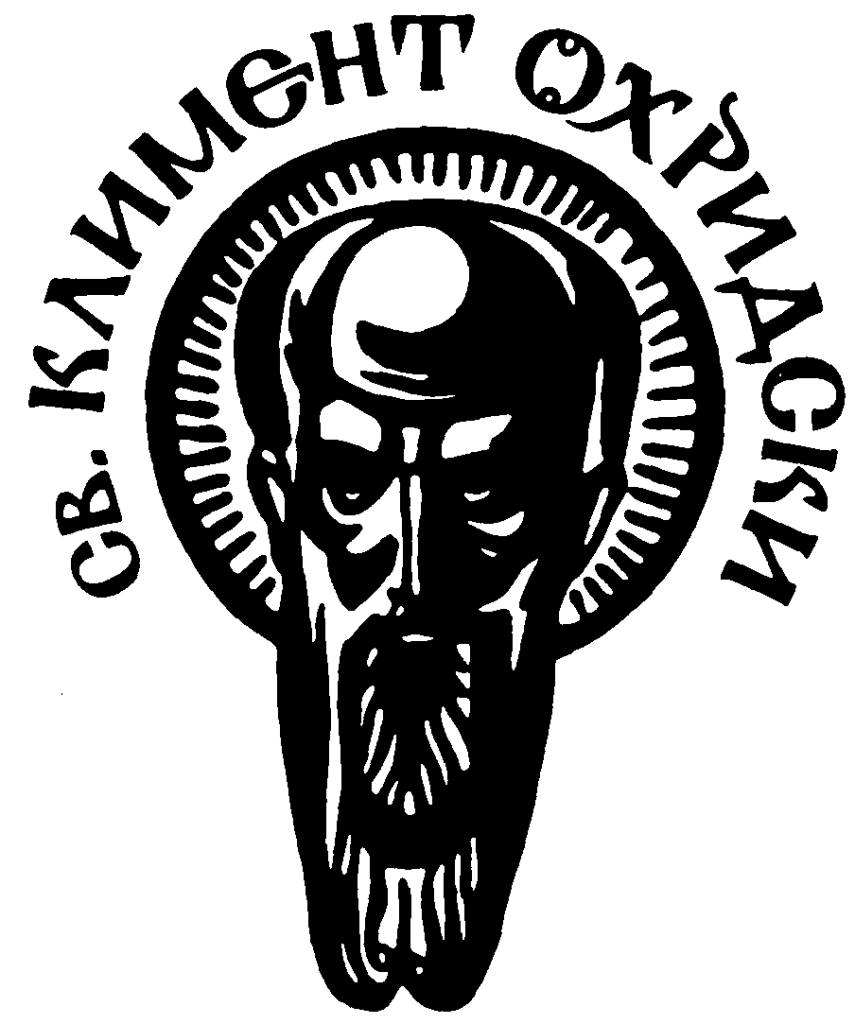
\includegraphics[width=0.4\textwidth]{su}
			
			\LARGE
			Факултет по математика и информатика\\
			Катедра "`Математическа логика и приложенията ѝ"'\\
			
			\vspace{0.9cm}
			Дипломна работа\\
			
			\vspace{1.3cm}
			{\color{blue}\hrule depth 0.05cm}
			\Huge
			\textbf{Оптимизиране на преизползването на паметта в програми на функционални езици за програмиране}
			\vspace{0.2cm}
			{\color{blue}\hrule depth 0.05cm}
			
			\vspace{1.3cm}
			\Large
			Илиян Йорданов\\
			
			\vspace{0.2cm}
			\begin{table}[ht]
				\vspace*{-0.2cm}
				\begin{tblr}{X[50,r,m]X[50,l,m]}
					\Large факултетен номер: & \Large 5MI3400037 \\ 
					\Large магистърска програма: & \Large "`Логика и алгоритми"' (инф.) \\ 
					& \\
					\Large Научен ръководител: & \Large проф. Стоян Михов \\
				\end{tblr}
			\end{table}
			
			\vspace{0.6cm}
			София, юли 2023 г.
		\end{center}
	\end{titlepage}
	\clearpage
	
	{
		\hypersetup{linkcolor=black}
		\tableofcontents
	}
	\clearpage
	
	\phantomsection
	\section*{Увод}
	\addcontentsline{toc}{section}{Увод}
	\markboth{Увод}{Увод}
	Управлението на паметта при реализирането на функционалните езици за програмиране се извършва чрез алгоритми за автоматично почистване на неизползваната памет. Те се наричат стандартно Garbage collection - "`събиране на боклук"'. Най-разпространеният метод се състои в периодично преглеждане на паметта и освобождаване на излишната заета памет. Този подход често води до съществено забавяне на програмите, поради което е актуална темата за разработване на алтернативни методи. Един от актуалните алтернативни методи е чрез използване на "`броячи на референции"' към паметта на обектите. Този подход позволява да се освобождава паметта в момента, когато към нея няма активни референции. Голямо предимство на метода е, че позволява паметта да се преизползва в някои случаи. Тогава вместо да се освобождава паметта, към която няма повече референции, може да се използва за някой текущо инициализиран обект.
	
	Разбира се метода с "`броячи на референции"' има и някои сериозни минуси като проблеми с идентифицирането на цикли от референции, допълнителното оскъпяване на основните операции за референции в конкурентна среда (защото трябва да са атомарни) и други. Но дори и в днешно време продължава да е актуална тема. Така в \cite{perseus} се показва нов алгоритъм за този метод, за който се твърди, че успява да се справи с част от негативите като цикли от референции. Също в тази статия се говори за предимството на метода от гледна точка на преизползването на памет и ресурси, което ще е главната цел на дипломната работа.
	
	Ще мислим, че говорим за функционални езици с Garbage collection тип "`броячи на референции"', за да е известно кога към някоя памет наистина няма повече референции и може да настъпи фактическо освобождаване или преизползване за друг обект. Описаните методи са удачни точно за такъв тип Garbage collection, защото имаме възможност да знаем, че към някоя памет няма повече активни референции, и вместо да я освободим можем да я преизползваме. Първо, ще изградим абстракция на функционалните езици, за да разсъждаваме най-общо, а не от гледната точка на фиксиран функционален език. След което ще фиксираме конкретна програма, защото нашата идея е да направим най-подходящ ред на изпълнение на изчисленията, така че да може да се възползваме от преизползването на памет. Така ще формулираме целева задача, която ще изследваме усилено, и ще докажем, че е в класа \texttt{NP-трудност}. Накрая, все пак ще предложим алгоритъм за намиране на подходящ ред на изчислението, така че да имаме някакви гаранции на преизползване на памет.
	
	\newpage
	
	\section{Основни понятия и означения}
	\fancypagestyle{style}{%
		\fancyhead[R]{0.1. Най-общи означения и символи}
	}
	\thispagestyle{style}
	
	В този раздел ще представим базовите понятия и знания, които ще използваме в цялата дипломната работа.
	
	\subsection{Най-общи означения и символи}
	\begin{denotations}[основни логически символи]~
		\begin{itemize}
			\item $\lnot$ - логическо "`не"';
			\item $\land$ - логическо "`и"';
			\item $\lor$ - логическо "`или"';
			\item $\implies$ със значението на следователно - "`ако ..., то ..."';
			\item $\iff$ със значението на тогава и само тогава;
			\item $\exists$ - съществува;
			\item $\forall$ - за всяко.
		\end{itemize}
	\end{denotations}
	
	\begin{denotations}[основни операции с множества]~
		\begin{itemize}
			\item $\in$ със значението "`... е елемент на множеството ..."';
			\item $\subseteq$ със значението "`всички елементи на множеството ... са елементи на множеството ..."';
			\item $\subset$ - със значението "`всички елементи на множеството ... са елементи на множеството ..., но има поне един елемента на второто множество, който не е в първото"' (не съвпадат изцяло).
		\end{itemize}
	\end{denotations}
	
	\begin{denotations}[основни математически символи в определения, доказателства и алгоритми]~
		\begin{itemize}
			\item $=$ със значението "`... е равно на ..."';
			\item $:=$ със значението "`... е дефинирано като ..."';
			\item $\gets$ със значението "`на ... се присвоява стойността ..."' (в контекста на описанието на алгоритми);
			\item БОО със значението "`без ограничение на общността"';
			\item $\lightning$ - със значението "`получихме противоречие"';
			\item $\square$ - със значението "`край на доказателството"'.
		\end{itemize}
	\end{denotations}
	
	\subsection{Общи понятия и означения от теория на множествата}
	\begin{denotations}[празно множество и някои бинарни операции с множества]~\\
		\indent Празното множество ще бележим с $\varnothing$. Ще използваме и следните допълнителни бинарни операции за множества:
		\begin{itemize}
			\item $A \cup B$ за означаване на множеството, съдържащо елементите, които са в множеството $A$ или в множеството $B$ (обединение на множества); 
			\item $A \cap B$ за означаване на множеството, съдържащо елементите, които са в множеството $A$ и в множеството $B$ (сечение на множества);
			\item $A \setminus B$ за означаване на множеството, съдържащо елементите, които са в множеството $A$, но не са в множеството $B$ (разлика на множества).
		\end{itemize}
	\end{denotations}
	
	\begin{denotations}[кардиналност на множество и естествени числа]~\\
		\indent Кардиналността (мощността) на дадено множество $A$, ще означаваме като $|A|$. Естествените числа ще отбелязваме с $\mathbf{N} := \{1, 2, \dots\}$, а с $\mathbf{N}_0 := \{0, 1, 2, \dots\}$ - естествените числа и нулата.
		
		\textit{Бележка}: Ние ще се занимаваме предимно с крайни множества, т.е. такива, за които $|A| \in \mathbf{N}_0$. При тях мощността е просто броя елементи в множеството. Ако едно множество не е крайно, то е безкрайно.
	\end{denotations}
	
	\begin{denotation}~\\
		\indent Ще използваме $[n]:=\{1, 2, \dots, n\}$ за означаване на множеството от първите $n \in \mathbf{N}_0$ естествени числа. Да поясним, че $[0]=\varnothing$.
	\end{denotation}
	
	\begin{denotation}[степенно множество]~\\
		\indent Степенното множество, съдържащо всички подмножества на дадено множество $A$, ще означаваме с $\mathcal{P}(A)$. Понеже ще работим най-вече с крайни множества, то предимно ще използваме $\mathcal{P}_{fin}(A)$, с което ще означаваме само крайните подмножества на $A$.
	\end{denotation}
	
	\begin{definition}[разбиване на множество]~\\
		\indent Нека имаме множеството $A$. Тогава разбиване на $A$ наричаме всяко множество $P \subseteq \mathcal{P}(A) \setminus \{\varnothing\}$ със свойствата:
		\begin{itemize}
			\item $\bigcup_{X \in P}X = A$;
			\item $(\forall X \in P)(\forall Y \in P)(X \neq Y \implies X \cap Y = \varnothing)$.
		\end{itemize}
		Така всеки елемент на $A$ е точно в едно от подмножествата в разбиването $P$.
	\end{definition}
	
	\begin{denotations}[декартово произведение на множества]~\\
		\indent Декартовото произведение на две множества $A$ и $B$, ще означаваме с $A \times B$, като в него се съдържат всички наредени двойки с първи елемент от множеството $A$ и втори елемент от множеството $B$. Ще означаваме наредена двойка с първи елемент $a$ и втори елемент $b$, като $(a,b)$. Съответно ще използваме означението $proj_1(\dots)$ за намиране на първия елемент и $proj_2(\dots)$ за намиране на втория елемент на наредена двойка, т.е. $proj_1((a,b))=a$ и $proj_2((a,b))=b$. Допълнително, ще въведем наредените $n$-торки $(a_1, a_2, \dots, a_n)$, които са елемент на $A_1 \times A_2 \times \dots \times A_n$ - декартовото произведение на множествата $A_1, A_2, \dots, A_n$ ($a_1 \in A_1, a_2 \in A_2, \dots, a_n \in A_n$) за $n \in \mathbf{N}$ и $n \ge 2$.
	\end{denotations}
	
	\newpage 
	\begin{denotation}[$n$-торка]~\\
		\indent За краткост, $n$-торката $(a_1, a_2, \dots, a_n) \in A^n$, където $A^n := \underbrace{A \times A \times \dots \times A}_n$, понякога ще записваме и като $\overline{a}^n$. Също в зависимост от контекста под $\overline{a}^n$ ще разбираме и просто изреждането $a_1, a_2, \dots, a_n$.
	\end{denotation}
	
	\begin{definition}[релация]~\\
		\indent Нека са дадени множествата $A_1, A_2, \dots, A_n$ за $n \in \mathbf{N}$ и $n \ge 2$. Тогава едно множество $R$ наричаме ($n$-местна) релация, ако: $R \subseteq A_1 \times A_2 \times \dots \times A_n$. Ако $n=2$, то още ще означаваме $(a,b) \in R$ като $aRb$.
	\end{definition}
	
	\begin{definitions}~\\
		\indent Нека е дадена релацията $R \subseteq A \times B$. Ще въведем някои основни понятия и означения за релации:
		\begin{itemize}
			\item $Dom(R) := \{a \in A \mid (\exists b \in B)((a,b) \in R)\}$ - дефиниционно множество на релацията $R$ (първите елементи в наредените двойки в $R$);
			\item $Rng(R) := \{b \in B \mid (\exists a \in A)((a,b) \in R)\}$ - област от стойности на релацията $R$ (вторите елементи в наредените двойки в $R$);
			\item $R[A'] := \{b \in B \mid (\exists a \in A')((a,b) \in R)\}$, където $A' \subseteq A$ - образите на множество елементи $A'$;
			\item $R^{-1} := \{(b, a) \mid (a,b) \in R\}$ - обратната релация на $R$, която е подмножество на $B \times A$;
			\item $R\restriction_{A'} := \{(a,b) \mid (a,b) \in R \land a \in A'\}$, където $A' \subseteq A$ - рестрикция на $R$ до подмножеството $A'$;
			\item $R$ е функционална релация, ако $(\forall a \in A)(\forall b_1 \in B)(\forall b_2 \in B)((a, b_1) \in R \land (a, b_2) \in R \implies b_1 = b_2)$.
		\end{itemize}
	\end{definitions}
	
	\begin{definitions}[релация на еквивалентност]~\\
		\indent Нека е дадена релацията $R \subseteq A \times A$. Ще въведем следните свойства на релациите:
		\begin{itemize}
			\item рефлексивност - $(\forall a \in A)((a,a) \in R)$;
			\item симетричност - $(\forall a \in A)(\forall b \in A)((a,b) \in R \implies (b,a) \in R)$;
			\item транзитивност - $(\forall a \in A)(\forall b \in A)(\forall c \in A)((a,b) \in R \land (b,c) \in R \implies (a,c) \in R)$.
		\end{itemize}
		
		Релация, която изпълнява горните три свойства, се нарича релация на еквивалентност.
	\end{definitions}
	
	\begin{definitions}[класове на еквивалентност и фактор-множество]~\\
		\indent Нека е дадена релацията $R \subseteq A \times A$ на еквивалентност. Тогава $[a]_R := \{b \in A \mid (a,b) \in R\}$ наричаме клас на еквивалентност на елемента $a$ относно релацията $R$.
		
		Множеството $\{[a]_R \mid a \in A\}$ с всички класове на еквивалентност ще наричаме фактор-множество на $A$ относно релацията $R$.
		
		\textit{Бележка}: Може да се докаже, че фактор-множеството на $A$ относно релацията $R$ представлява разбиване на множеството $A$.
	\end{definitions}
	
	\begin{definition}[функция]~\\
		\indent Функциите ще разглеждаме като релации, които са функционални. Ще означаваме $f \colon A \to B$ за функция с домейн множеството $A$ и кодомейн множеството $B$ - $f \subseteq A \times B$. Ще записваме $f(a)=b$ вместо $(a,b) \in f$.
		
		\textit{Бележка}: Тази дефиниция е много обща и позволява функцията да не е дефинирана за всеки елемент на домейна, както и да не съпоставя всяка стойност в кодомейна, т.е. $Dom(f) \subseteq A$ и $Rng(f) \subseteq B$.
	\end{definition}
	
	\begin{definition}[$n$-местна функция]~\\
		\indent Нека имаме функцията $f \colon A \to B$ за множествата $A$ и $B$. Ако множеството $A$ е $n$-местна релация за $n \in \mathbf{N}$ и $n \ge 2$, то ще наричаме $f$ още $n$-местна функция. За по-кратко при $(a_1, a_2, \dots, a_n) \in A$ ще записваме $f(a_1, a_2, \dots, a_n)$ вместо $f((a_1, a_2, \dots, a_n))$.
	\end{definition}
	
	\begin{definitions}~\\
		\indent Нека е дадена функцията $f \colon A \to B$. Ще въведем някои основни понятия за функции:
		\begin{itemize}
			\item ако $Dom(f) \subseteq A$, то казваме, че функцията $f$ е частична;
			\item ако $Dom(f) = A$, то казваме, че функцията $f$ е тотална;
			\item ако $(\forall a_1 \in A)(\forall a_2 \in A)(f(a_1) = f(a_2) \implies a_1 = a_2)$, то казваме, че функцията $f$ е инекция;
			\item ако $(\forall a_1 \in A')(\forall a_2 \in A')(f(a_1) = f(a_2) \implies a_1 = a_2)$ за $A' \subseteq A$, то казваме, че функцията $f$ е инективна върху множеството $A'$;
			\item ако $Rng(f) = B$, то казваме, че функцията $f$ е сюрекция;
			\item ако $f$ е инекция и сюрекция, то казваме, че $f$ е биекция;
			\item ако $f$ е инекция, то $f^{-1}$ - обратната релация на $f$, ще наричаме просто обратна функция. (може да се покаже, че наистина е функция).
		\end{itemize}
		
		\textit{Бележка}: По-нататък под функция ще разбираме тотална функция освен ако явно не е казано, че говорим за частична функция.	Нека имаме краен домейн $A$. Тогава може да се докаже, че ако $A' \subseteq A$, то $|f[A']| \le |A'|$. Ако $f$ e инективна върху множеството $A'$, то $|f[A']| = |A'|$. Също ако $A' \subseteq A$ и $f$ е инективна функция, то може да се покаже, че $f\restriction_{A'} \colon A' \to B$ е също инекция. 
	\end{definitions}
	
	\begin{definitions}[изброимо множество]~\\
		\indent Едно множество $A$ наричаме изброимо, ако има инекция между $A$ и $\mathbf{N}$. Ако има и биекция между $A$ и $\mathbf{N}$, то $A$ се нарича още изброимо безкрайно множество.
	\end{definitions}
	
	\begin{definition}[редица]~\\
		\indent Ако имаме функцията $a \colon [n] \to A$ за $n \in \mathbf{N}_0$ и множеството $A$, то ще наричаме още $a$ редица и ще бележим, като $(a_k)_{k=1}^{n}$. Съответно $a_k=a(k)$ за $k \in [n]$. Също само $a$ ще приемаме и като означение за цялата редица $a_1, a_2, \dots, a_n$. Този вид редици ще наричаме крайни и $n$ е дължината на редицата.
		
		Нека имаме функцията $a \colon \mathbf{N} \to A$ за множеството $A$. Тогава $a$ ще наричаме още безкрайна редица и ще бележим, като $(a_k)_{k=1}^\infty$. Отново $a_k=a(k)$ за $k \in \mathbf{N}$ и само $a$ ще приемаме като означение за цялата редица $a_1, a_2, \dots$.
		
		\textit{Бележка}: Понякога редицата ще започваме от 0 - $(a_k)_{k=0}^{n}$ за $n \in \mathbf{N}_0$, като тогава може да разглеждаме, че изхождаме от функцията $a \colon \{0\} \cup [n] \to A$ и дължината е $n+1$.
	\end{definition}
	
	\begin{definition}[конкатенация на две крайни редици]~\\
		\indent Нека имаме двете крайни редици $(a_i)_{i=1}^n$ и $(b_j)_{j=1}^m$ за $n,m \in \mathbf{N}_0$. Тогава редицата $(c_h)_{h=1}^{n+m}$, за която $c := a_1, a_2, \dots, a_n, b_1, b_2, \dots, b_m$ наричаме конкатенация на двете редици. Освен това ще бележим, че $c = a \cdot b$.
	\end{definition}
	
	\subsection{Общи понятия и означения от теория на формалните езици}
	\begin{definition}[азбука]~\\
		\indent Всяко крайно множество ще наричаме азбука. Обикновено ще бележим азбуката със $\Sigma$, а елементите на това множество ще наричаме символи.
	\end{definition}
	
	Нека фиксираме една азбука $\Sigma$.
	
	\begin{definition}[дума]~\\
		\indent Всяка крайна редица от елементи на азбуката $\Sigma$, включително и редица без елементи, ще наричаме дума. Стандартно ще означаваме думите с $\alpha, \beta, \gamma, \gamma_1, \gamma_2, \dots$ и ще казваме, че те са думи над $\Sigma$.
	\end{definition}
	
	\begin{definition}[конкатенация на думи]~\\
		\indent Нека имаме две думи $\alpha$ и $\beta$ над $\Sigma$. Тогава конкатенация на думите наричаме думата $\gamma$, която представлява конкатенираната редица от символи на съответните редици на $\alpha$ и $\beta$. Стандартно ще означаваме, че $\gamma = \alpha \cdot \beta$.
	\end{definition}
	
	\begin{denotation}[поддума]~\\
		\indent Казваме, че думата $\alpha$ е поддума на думата $\beta$, ако $\beta = \gamma_1 \cdot \alpha \cdot \gamma_2$ за някои две думи $\gamma_1$ и $\gamma_2$ над $\Sigma$.
	\end{denotation}
	
	\subsection{Общи понятия и означения за логическите езици от първи ред}
	\begin{definition}[сигнатурен език]\label{def:RFOL}~\\
		\indent Сигнатурният език ще се състои от няколко азбуки, функцията $\#$ и термове:
		\begin{itemize}
			\item азбука за всички индивидни константи, които ще бележим с $c, c_0, c_1, \dots$;
			\item азбука за всички функционални символи, които ще бележим с $f, g, h, F, G, H,$ $f_0, g_0, h_0, F_0, G_0, H_0, f_1, g_1, h_1, F_1, G_1, H_1, \dots$;
			\item изброимо безкрайната азбука за всички индивидни променливи, които ще бележим с $X, Y, Z, X_0, Y_0, Z_0, X_1, Y_1, Z_1, \dots$;
			\item азбука за допълнителни символи $\{, , (, )\}$ (първият елемент на множеството е символът запетайка).
		\end{itemize}
		Функцията $\#$ е с домейн азбуката за всички функционални символи и кодомейн $\mathbf{N}$ и тази функция за всеки функционален символ връща броя аргументи, които приема символът. Още ще наричаме този брой арност на функционалния символ. Множеството от всички символи от азбуките в първите две точки ще наричаме сигнатура на езика. Термовете ще бъдат обектите на езика, като тях ще дефинираме формално в следващото определение.
		
		Стандартно ще означаваме сигнатурен език с $\mathcal{L}$ и евентуално $\mathcal{L}$ с индекс.
		
		\textit{Бележка}: Това определение реално е ограничено определение за логически език от първи ред, при който имаме допълнително азбуки за логически и предикатни символи и формули. Понеже в рамките на дипломната работа ще работим с езици от първи ред, без да разглеждаме формули, ще въведем само този вид езици, които наричаме сигнатурни езици, защото реално в тях е само сигнатурата на логически език от първи ред и индивидните променливи.
	\end{definition}
	
	Нека фиксираме сигнатурен език $\mathcal{L}$ до края на подраздела.
	\begin{definition}[терм]\label{def:term}~\\
		\indent Стандартно ще бележим термовете с $\tau, \tau', \tau_0, \tau_0', \tau_1, \tau_1', \dots$. Терм ще дефинираме индуктивно, както следва:
		\begin{itemize}
			\item $c$ е терм, където $c$ е символ за индивидна константа;
			\item $X$ е терм, където $X$ е символ за индивидна променлива;
			\item $f(\tau_1,\tau_2,\dots,\tau_m)$ е терм, където $f$ е функционален символ с арност $m$.
		\end{itemize}
		Термовете от първите две точки ще наричаме атомарни, а от последната - неатомарни.
	\end{definition}
	
	\begin{denotation}[аргумент на неатомарен терм]~\\
		\indent Нека имаме неатомарен терм $\tau = f(\tau_1,\tau_2,...,\tau_m)$ за функционален символ $f$ с арност $m$. Тогава ще използваме следното означение за това, че термът има аргумент $\tau_i$ на позиция $i \in [m]$: $f(\dots,\overset{i}{\tau_i},\dots)$.
	\end{denotation}
	
	\begin{denotation}[аргументи на функционален символ]~\\
		\indent Нека имаме функционален символ $f$ с арност $m$. Тогава, ако имаме редицата $(a_k)_{k=1}^{m}$ от термове, то под $f(a)$ ще разбираме $f(a_1, a_2, \dots, a_m)$, където $a$ представлява редицата от аргументи на функционалния символ $f$.
	\end{denotation}
	
	\newpage
	\begin{denotation}[еднакви термове]~\\
		\indent Нека имаме термовете $\tau_1$ и $\tau_2$. Ще бележим $\tau_1 = \tau_2$, ако двата терма съвпадат посимволно (т.е. са еднакви разгледани като думи над обединението на азбуките за индивидни константи, индивидни променливи и допълнителните символи).
	\end{denotation}
	
	Лесно може да се покаже, че ако $\tau$ е терм, то е изпълнено точно едно от следните:
	\begin{itemize}
		\item съществува единствена константа, за която $\tau = c$;
		\item съществува единствена променлива, за която $\tau = X$;
		\item съществува единствен функционален символ, за който $\tau = f(\dots)$ - единствената възможност за неатомарен терм.
	\end{itemize}
	
	\begin{definition}[затворен терм]~\\
		\indent Един терм $\tau$ ще наричаме затворен, ако в него няма символи за индивидни променливи.
	\end{definition}
	
	\begin{definitions}[подтерм и непосредствен подтерм]\label{def:subterm}~\\
		\indent Нека имаме терма $\tau$. Тогава термът $\tau'$ е подтерм на $\tau$, ако $\tau'$ е поддума на $\tau$, разгледано посимволно. Ако $\tau = f(\dots, \tau', \dots)$, то наричаме $\tau'$ още непосредствен подтерм на $\tau$.
	\end{definitions}
	
	Лесно може да се убедим, че ако $\tau'$ е подтерм на $\tau = f(\tau_1, \tau_2, \dots, \tau_m)$, където $f$ е функционален символ с арност $m$, то е в сила точно едно от следните:
	\begin{itemize}
		\item $\tau' = \tau$;
		\item $\tau'$ е подтерм на някое $\tau_i$ за $i \in [m]$.
	\end{itemize}
	
	\begin{denotations}[подтерм и непосредствен подтерм]~\\
		\indent Ще използваме следните означения:
		\begin{itemize}
			\item $\tau' \le \tau$ за това, че $\tau'$ е подтерм на $\tau$;
			\item $\tau' \prec \tau$ за това, че $\tau'$ е непосредствен подтерм на $\tau$;
			\item $\tau' < \tau$ за това, че $\tau'$ е строг подтерм на $\tau$ (строг подтерм означава, че $\tau'$ е подтерм на $\tau$, но не съвпада посимволно с него).
		\end{itemize}
	\end{denotations}
	
	След като въведохме синтаксиса на ограничените езици от първи ред, ще поговорим за семантиката, като въведем понятието структура на сигнатурен език.
	
	\begin{definition}[структура на сигнатурен език]\label{def:struct}~\\
		\indent Нека имаме сигнатурен език $\mathcal{L}$. Тогава структура \textfrak{A}, ще е наредената двойка $(\mathbf{U}, \mathbf{I})$, така че:
		\begin{itemize}
			\item $\mathbf{U}$ е непразно множество, което ще наричаме носител (универсум) на структурата;
			\item $\mathbf{I}$ е съответствие, което предава семантиката на символите от сигнатурата на $\mathcal{L}$ спрямо универсума $\mathbf{U}$ и ще наричаме интерпретация;
			\item за всяка индивидна константа $c$, $\mathbf{I}(c) := c^\textfrak{A} \in \mathbf{U}$;
			\item за всеки функционален символ $f$, $\mathbf{I}(f) := f^\textfrak{A}$, като $f^\textfrak{A}: \mathbf{U}^m \to \mathbf{U}$, където $m$ е арността на $f$; така всеки функционален символ се интерпретира като функция.
		\end{itemize}
		
		Стандартно ще означаваме структурата за сигнатурен език с \textfrak{A} и евентуално \textfrak{A} с индекс.
	\end{definition}
	
	Нека сме фиксирали и структурата $\textfrak{A} = (\mathbf{U}, \mathbf{I})$ за езика $\mathcal{L}$ до края на подраздела.
	
	\begin{definition}[стойност на затворен терм]~\\
		\indent Стойност на затворен терм $\tau$ в структурата $\textfrak{A}$ ще бележим с $\llbracket\tau\rrbracket^\textfrak{A}$ и ще представлява интерпретацията, която структурата дава на терма. Тази интерпретация ще дефинираме индуктивно, както следва:
		\begin{itemize}
			\item ако $\tau = c$ за някоя константа, то стойността е $c^\textfrak{A}$;
			\item ако $\tau = f(\tau_1,\tau_2,\dots,\tau_m)$ за някой функционален символ $f$ с арност $m$, то стойността е $f^\textfrak{A}(\llbracket\tau_1\rrbracket^\textfrak{A},\llbracket\tau_2\rrbracket^\textfrak{A},\dots,\llbracket\tau_m\rrbracket^\textfrak{A})$.
		\end{itemize}
	\end{definition}
	
	\begin{definition}[обогатяване на сигнатурен език]~\\
		\indent Нека имаме сигнатурен език $\mathcal{L}_1$. Тогава ще казваме, че $\mathcal{L}_1$ обогатява $\mathcal{L}$, ако сигнатурата на $\mathcal{L}$ е подмножество на сигнатурата на $\mathcal{L}_1$.
		
		\textit{Бележка}: В рамките на дипломната работа, единственото обогатяване на сигнатурен език ще е добавянето на нови функционални символи.
	\end{definition}
	
	Нека езика от първи ред $\mathcal{L}_1$ е обогатяване на езика $\mathcal{L}$. Тогава, за да получим структура $\textfrak{A}_1$ за $\mathcal{L}_1$, можем просто да разширим структурата $\textfrak{A}$ за $\mathcal{L}$ с интерпретации на новите индивидни константи и функционални символи.
	
	\subsection{Общи понятия и означения от теория на графите}
	Ще въведем единствено ориентирани графи, защото няма да има нужда да работим с неориентирани.
	\begin{definition}[ориентиран граф]~\\
		\indent Ориентиран граф е наредена двойка $G=(V,E)$, където $V$ е непразно множество, чиито елементи наричаме върхове, а $E$ е множество, чиито елементи наричаме ребра, и $E \subseteq V \times V$.
		
		\textit{Бележка}: По-нататък ще използваме главно графи с етикети по ребрата, които ще са тройка - $G=(V,E,l)$, където $l$ е функция, която задава етикети на ребрата. Всички понятия по-нататък, които са за графи без етикети, можем да считаме и за понятия на графите с етикети по ребрата.
	\end{definition}
	
	\begin{definition}[примка]~\\
		\indent Нека е даден граф $G=(V,E)$. Едно ребро $(u,v) \in E$ наричаме примка, ако $u=v$.
		
		\textit{Бележка}: Определението ни за ориентиран граф е по-общо и позволява да имаме примки, което ще ограничим със следващото определение.
	\end{definition}
	
	\begin{definition}[прост граф]~\\
		\indent Един граф се нарича прост, ако няма примки и не е мултиграф.
		
		\textit{Бележка}: Определението ни за ориентиран граф не позволява той да е мултиграф, т.е. да има повече от едно ребро между една и съща наредена двойка върхове. Така че, ако един ориентиран граф е прост, единственото реално ограничение е да няма примки.
	\end{definition}
	
	От сега до края на подраздела ще фиксираме прост ориентиран граф $G=(V,E)$.
	\begin{definitions}~\\
		\indent Нека разгледаме едно произволно ребро $e = (u,v) \in E$. Тогава имаме следните понятия:
		\begin{itemize}
			\item върха $u$ наричаме входящ връх за реброто $e$ и обратно казваме, че реброто $e$ е излизащо от връх $u$;
			\item върха $v$ наричаме изходящ връх за реброто $e$ и обратно казваме, че реброто $e$ е влизащо за връх $v$;
			\item върха $v$ наричаме съсед на връх $u$.
		\end{itemize}
	\end{definitions}
	
	\begin{definitions}[подграф и индуциран подграф]~\\
		\indent Един граф $G'=(V',E')$ наричаме подграф на $G=(V,E)$, ако $V' \subseteq V$ и $E' \subseteq E$. Нека да уточним, че $G'$ е граф, т.е. трябва $E' \subseteq V' \times V'$.
		
		Нека разгледаме едно непразно подмножество $U \subseteq V$. Тогава подграфът, индуциран от $U$, е графът $G^{ind}=(U, E^{ind})$, където $E^{ind} := \{(u,v) \in E \mid u \in U \land v \in U\}$.
	\end{definitions}
	
	\newpage
	\begin{definitions}[път и цикъл в граф]~\\
		\indent Път в граф ще наричаме редица от върхове $u_0, u_1, \dots, u_k$ за $k \ge 0$, така че $(u_0, u_1) \in E, (u_1, u_2) \in E, \dots, (u_{k-1}, u_k) \in E$. Върха $u_0$ наричаме начало на пътя, върха $u_k$ - край на пътя и казваме, че пътят е от връх $u_0$ до връх $u_k$. Също в случая казваме, че върхът $u_k$ е достижим от върха $u_0$. Дължината на пътя е броят ребра в него - $k$. Ако върховете в пътя не се повтарят, то наричаме пътя прост.
		
		Един път в графа се нарича още цикъл, ако началото и краят му съвпадат, и също така дължината му е поне $2$ (т.е. има поне $3$ върха).
	\end{definitions}
	
	\begin{definitions}[предшественик и наследник]~\\
		\indent Нека е даден произволен връх $u \in V$ и разглеждаме друг връх $v \neq u \in V$. Тогава:
		\begin{itemize}
			\item $v$ се нарича предшественик на $u$, ако има път от $v$ до $u$, а ако има път с дължина $1$, наричаме $v$ още непосредствен предшественик;
			\item $v$ се нарича наследник на $u$, ако има път от $u$ до $v$, а ако има път с дължина $1$, наричаме $v$ още непосредствен наследник.
		\end{itemize}
	\end{definitions}
	
	\begin{definitions}[функции за непосредствените предшественици и наследници на връх]~\\
		\indent Нека имаме ориентиран граф $G$ с върхове $V$. Тогава:
		\begin{itemize}
			\item функцията $A_G\colon V \to \mathcal{P}(V)$, дефинирана като $A_G(v):=\{u \mid (u, v) \in E\}$ за всяко $v \in V$, връща непосредствените предшественици на всеки връх;
			\item функцията $D_G\colon V \to \mathcal{P}(V)$, дефинирана като $D_G(v):=\{u \mid (v, u) \in E\}$ за всяко $v \in V$, връща непосредствените наследници (съседите) на всеки връх.
		\end{itemize}
		
		\textit{Бележка}: Името на функциите идва от първите букви на английските думи \textit{ancestor} и \textit{descendant}, съответно.
	\end{definitions}
	
	\begin{definition}[ацикличен граф]~\\
		\indent Един граф се нарича ацикличен, ако няма цикъл.
		
		\textit{Бележка}: Лесно може да се покаже, че в ацикличен граф винаги има поне един връх без непосредствени предшественици (или съответно без влизащи ребра).
	\end{definition}
	
	\begin{definition}[топологична наредба на ацикличен граф]~\\
		\indent Нека $n=|V|$ е броят върхове на графа. Тогава биекцията $t\colon V \to [n]$ наричаме топологична наредба, ако изпълнява свойството: $(\forall (u,v) \in E)(t(u)<t(v))$.
		
		\textit{Бележка}: Ще наричаме топологичната наредба и топологично сортиране. Освен това, понякога ще разглеждаме топологичната наредба $t$ като редицата: $t_1 = t^{-1}(1), t_2 = t^{-1}(2), \dots, t_n = t^{-1}(n)$, защото по същество е просто пермутация на върховете на графа.
	\end{definition}
	
	Лесно може да се докаже, че един граф е ацикличен тогава и само тогава, когато има топологична наредба. Освен това тя има допълнителното свойство, че за всеки връх освен че всички непосредствени предшественици са преди него в наредбата, въобще всички негови предшественици са преди него в наредбата.
	
	\newpage
	\begin{definitions}[силна свързаност]~\\
		\indent За два върха $u, v \in V$ казваме, че са силно свързани, ако има път от $u$ до $v$ и път от $v$ до $u$. Един ориентиран граф се нарича силно свързан, ако изпълнява свойството: $(\forall u \in V)(\forall v \in V)(u\text{ и }v\text{ са силно свързани})$, 
	\end{definitions}
	
	Нека въведем релацията на силна свързаност $R := \{(u, v) \in V \times V \mid u\text{ и }v$ са силно свързани$\}$. Лесно може да се покаже, че тази релация изпълнява нужните свойства и е релация на еквивалентност.
	
	\begin{definition}[кондензиран граф]~\\
		\indent Подграфите на $G$, индуцирани от класовете на еквивалентност на релацията силна свързаност, се наричат силно свързани компоненти. Стандартно ще означаваме множествата на върховете на силно свързаните компоненти на ориентиран граф с $C_1, C_2, \dots, C_k$ (те представляват разбиване на върховете $V$ и $1 \le k \le |V|$).
		
		Нека $V^{cond} := \{C_1, C_2, \dots, C_k\}$ е множеството от множествата на върховете на силно свързаните компоненти (още фактор-множеството относно релацията силна свързаност). Тогава, ако $E^{cond} := \{(C_i, C_j) \mid i \neq j \in [k] \land (\exists u \in C_i)(\exists v \in C_j)((u,v) \in E)\}$, то графа $G^{cond}=(V^{cond},E^{cond})$ наричаме кондензиран граф на $G$.
		
		\textit{Бележка}: Може да се докаже, че всеки кондензиран граф е ацикличен.
	\end{definition}
	
	\begin{definition}[изоморфни графи]~\\
		\indent Нека разгледаме два графа $G_1=(V_1,E_1)$ и $G_2=(V_2,E_2)$. Тогава изоморфизъм между $G_1$ и $G_2$ е всяка биективна функция $\varphi$ със свойството: $(\forall u \in V_1)(\forall u \in V_2)((u,v) \in E_1 \iff (\varphi(u),\varphi(v)) \in E_2)$. В този случай казваме, че графите $G_1$ и $G_2$ са изоморфни и бележим като $G_1 \cong G_2$.
		
		\textit{Бележка}: Ще използваме и понятието структура на графа, под което разбираме само върховете и ребрата му (без етикети, ако има) и освен това начина, по който ребрата свързвах върховете от гледна точка еднаквост с точност до изоморфизъм.
	\end{definition}
	
	Изоморфизмът между графи е много важно свойство, защото той на практика показва, че двата графа са едни и същи само с различни имена на върховете. Това означава, че имат едни и същи свойства. Така например, ако единият граф е ацикличен и другият е, ако единият е силно свързан и другият е и т.н.
	
	Ще въведем специален вид графи, които ще са важни за представяне на изчислението на термове - дървета. Ще използваме индуктивна дефиниция. \begin{definition}[кореново ориентирано дърво]~
		\begin{itemize}
			\item Графът $T=(V,E)$ е дърво с корен $r$, ако $V=\{r\}$ и $E=\varnothing$.
			\item Нека по индукционно предположение имаме дърветата $T_1=(V_1,E_1)$ с корен $r_1 \in V_1$, $T_2=(V_2,E_2)$ с корен $r_2 \in V_2$, \dots, $T_m=(V_m, E_m)$ с корен $r_m \in V_m$ за $m \ge 1$. Тогава, ако $V_i \cap V_j = \varnothing$ за всяко $1 \le i < j \le m$ и върхът $r \notin \bigcup_{i \in [m]}V_i$, то графът $T = (V,E)$ е дърво с корен $r$, където $V := \bigcup_{i \in [m]}V_i \cup \{r\}$ и $E := \bigcup_{i \in [m]}E_i \cup \{(r, r_i) \mid i \in [m]\}$.
		\end{itemize}
	\end{definition}
	
	\newpage
	\begin{definition}[поддърво]~\\
		\indent Нека имаме връх $r' \in V$ за кореновото дърво $T=(V,E)$. Тогава, ако $V' := \{v \in V \mid \exists \ \text{път от} \ r' \ \text{до} \ v\}$, то индуцирания подграф $T'(V',E')$ на $T$ относно върховете $V'$, наричаме поддърво на връх $r'$ в $T$, като $r'$ се явява корен на $T'$, който граф е кореново дърво.
	\end{definition}
	
	Ще дефинираме няколко понятия, които ще са ни удобни по-нататък.
	
	\begin{definitions}[листа, деца и родители]~\\
		\indent Нека имаме кореново дърво $T=(V,E)$ с корен $r \in V$ и разглеждаме произволен връх $v \in V$. Тогава:
		\begin{itemize}
			\item ако $D_T(v) = \varnothing$, то наричаме върха $v$ листо;
			\item ако $D_T(v) \neq \varnothing$, то съседите на връх $v$ - върховете от $D_T(v)$, наричаме още деца на върха $v$, а него наричаме родител на върховете от $D_T(v)$.
		\end{itemize}
		
		\textit{Бележка}: Може да се покаже, че в дърво, всеки връх без корена има точно един родител.
	\end{definitions}
	
	\begin{definition}[дълбочина на връх]~\\
		\indent Нека имаме кореново дърво $T=(V,E)$ с корен $r \in V$ и произволен връх $v \in V$. Тогава дълбочина на върха наричаме дължината на простия път от $r$ до връх $v$. (може да се покаже, че има точно един прост път от корена до всеки връх в кореново дърво)
	\end{definition}
	
	\subsection{Общи понятия и означения от теория на изчислителната сложност}
	
	\begin{denotations}~\\
		\indent Ще означаваме изчислителните задачите с $P, P', P_1, P_2$ и $P_3$. Изчислителните задачи ще имат безкрайно множество от възможни входове, които ще наричаме още екземпляри на задачите и ще бележим с $I$.
	\end{denotations}
	
	Ще разглеждаме два основни вида изчислителни задачи - задачи за разпознаване и оптимизационни изчислителни задачи. Екземплярите на една задача за разпознаване, които тя "`разпознава"', ще наричаме положителни екземпляри, а другите - отрицателни екземпляри.
	
	Нека разгледаме една оптимизационна задача $P$. БОО оптимизацията е за максимум. Лесно можем да получим съответна задача за разпознаване $P'$, като добавим всяко възможно число $k$ към всеки екземпляр $i$ на задача $P$, и задачата $P'$ е отговорът на въпроса "`Има ли допустимо решение в оригиналната задача на екземпляр $i$ с цена $\ge k$?"' Наричаме тази задача за разпознаване още версия за разпознаване на оптимизационната задача $P$. 
	
	Можем да си мислим за алгоритмите като средство (най-общо казано поредица от стъпки) как да представим една задача, така че тя да може да бъде успешно решена за всеки свой екземпляр от машина. Когато говорим за алгоритми, полученият екземпляр се нарича обикновено вход, а намереното решение - изход на алгоритъма.
	
	Едни от най-важните характеристики на алгоритмите са коректност и ефикасност. Алгоритъм е коректен, когато той намира вярно решение за всеки възможен екземпляр (спрямо задачата).
	
	За да мерим ефикасността на алгоритмите, ще използваме понятието сложност. Определянето на сложността изисква оценка на големината на входа. Грубо казано големината на входа е мярка за броя елементарни съставни части. Например, ако трябва да сортираме масив, обикновено големината на входа е просто броя числа (макар теоретично числата да могат да са огромни и представянето им да е много по-голямо от бройката им). Стандартно големината на входа ще бележим с $n \in \mathbf{N}_0$.
	
	Нека имаме конкретен алгоритъм $A$. Тук има три основни вида оценка по сложност - в най-добрия случай, в средния случай и в най-лошия случай. Разликата между тях е в това как ще анализираме поведението на алгоритъма при различни входни данни с един и същ размер на входа $n$. В рамките на дипломната работа винаги ще се интересуваме от поведението на алгоритмите в най-лошия случай или неформално казано от най-големия брой стъпки, които могат да са им необходими, за да намерят вярно решение за всеки вход с размер $n$. Поради различни причини се използва по-практическо означение за сложност на алгоритми. Указва се асимптотична горна граница на сложността, която се задава като функция от големината на входа чрез нотацията $O(\dots)$.
	
	\begin{definition}[асимптотична нотация голямо $O$]~\\
		\indent $O(g(n)) := \{f(n) \mid (\exists c \in \mathbf{N})(\exists n_0 \in \mathbf{N})(\forall n \ge n_0)(f(n) \le c.g(n))\}$. Ако $f(n) \in O(g(n))$ казваме, че $g(n)$ е асимптотична горна граница на функцията $f(n)$.
	\end{definition}
	Така ако кажем, че един алгоритъм в най-лошия си случай е $O(n^2)$, разбираме, че ако за всяка големина на входа $n \ge n_0$, разгледаме най-лошия възможен вход с тази големина, алгоритъмът ще работи грубо най-много $c.n^2$ на брой стъпки, където $c$ е някаква положителна константа, независеща от $n$. Освен това обикновено в тази нотация избягваме писането на коефициенти или добавяне на конкретни числа, така че вместо например $O(5.n^2+3)$ винаги ще пишем $O(n^2)$, а и двете множества от функции реално са едни и същи по определението. Разбира се, като оценяваме сложността на алгоритми в най-лошия случай с тази нотация, ще се стремим да намираме асимптотично най-малката възможна функция, за която все пак може да докажем, че е горна граница за сложността на нашия алгоритъм.
	
	От сега нататък, в рамките на цялата дипломна работа, под сложност на алгоритъм ще разбираме винаги сложност на алгоритъма в най-лошия случай. Ще ни е полезно да познаваме основните класове на сложност за задачите, които могат да бъдат решени пълно или частично с алгоритми. Затова ще въведем основните.
	
	\begin{definition}[полиномиален алгоритъм]~\\
		\indent Един алгоритъм $A$ наричаме полиномиален, ако сложността му е $O(n^k)$ за $k \ge 0$, където $n$ е големината на входа.
	\end{definition}
	
	\begin{definition}[класът \texttt{P}]~\\
		\indent Класът на сложност \texttt{P} съдържа всички задачи за разпознаване, за които има полиномиален алгоритъм. 
	\end{definition}
	
	Може да се каже, че класът \texttt{P} съдържа задачите за разпознаване, за които е намерен алгоритъм, който е сравнително ефикасен.
	
	\begin{definition}[класът \texttt{NP}]~\\
		\indent Класът на сложност \texttt{NP} съдържа всички задачи за разпознаване, за които има полиномиален алгоритъм, който за всеки положителен екземпляр може да провери всяко доказателство за положителния отговор.
	\end{definition}
	
	Известно е, че $\texttt{P} \subseteq \texttt{NP}$ и големият въпрос е дали са равни тези класове сложности.
	
	\begin{definition}[полиномиална сводимост]~\\
		\indent Нека имаме задачите за разпознаване $P_1$ и $P_2$ със съответните множества от екземпляри $I_1$ и $I_2$. Полиномиална сводимост на задача $P_1$ в задача $P_2$ е всяка функция $f: I_1 \to I_2$ със свойствата:
		\begin{itemize}
			\item $(\forall i \in I_1)(i\text{ е положителен екземпляр за }P_1 \iff f(i)\text{ е положителен екземпляр за }$ $P_2)$;
			\item има полиномиален алгоритъм, който може за всеки вход $i \in I_1$, да намери $f(i)$.
		\end{itemize}
		Полиномиалната сводимост от $P_1$ в $P_2$ ще означаваме като $P_1 \le_p P_2$.
	\end{definition}
	
	При изучаването на класа $\texttt{NP}$ се е появила една категория задачи, които са много централни и могат да се нарекат "`най-трудните"'.
	
	\begin{definition}[класът \texttt{NP-пълнота}]
		\indent Класът на сложност \texttt{NP-пълнота} съдържа всички изчислителни задачи за разпознаване $P$ със свойствата:
		\begin{itemize}
			\item $P \in \texttt{NP}$;
			\item $(\forall P' \in \texttt{NP})(P' \le_p P)$. 
		\end{itemize}
	\end{definition}
	
	Така задачите, които са \texttt{NP-пълни}, са най-централните, защото ако случайно имахме полиномиално решение за някоя от тях, то ще можем да го превърнем в решение на всяка друга задача от класа \texttt{NP}. Нека да отбележим, че за да докажем \texttt{NP-пълнотата} на една задача за разпознаване е достатъчно да сведем полиномиално някоя известна \texttt{NP-пълна} задача към нашата, защото полиномиалната сводимост, разгледана като релация между изчислителни задачи за разпознаване, е транзитивна ($P_1 \ge_p P_2 \land P_2 \ge P_3 \implies P_1 \ge P_3$).
	
	\begin{definition}[класът \texttt{NP-трудност}]~\\
		\indent Класът на сложност \texttt{NP-трудност} съдържа всички изчислителни задачи за разпознаване $P$ със свойството: $(\forall P' \in \texttt{NP})(P' \le_p P)$ и всички оптимизационни изчислителни задачи, чиято версия за разпознаване е \texttt{NP-трудна} задача.
		
		\textit{Бележка}: По принцип има различни разбирания относно оптимизационните задачи. Понеже по определение класът на \texttt{NP-трудните} задачи не е задължително да съдържа само \texttt{NP} задачи, то е удачно там да са подходящите "`сложни"' оптимизационни задачи.
	\end{definition}
	
	Последно ще формулираме една класическа оптимизационна \texttt{NP-трудна} задача, която ще използваме по-късно.
	
	\begin{definition}[върхово покритие]~\\
		\indent Нека е даден прост ориентиран граф $G=(V,E)$. Едно подмножество $U \subseteq V$ наричаме върхово покритие на графа, ако е изпълнено: $(\forall (u,v) \in E)(u \in U \lor v \in U)$.
	\end{definition}
	
	\begin{problem}[минимално върхово покритие] Нека е даден прост ориентиран граф $G=(V,E)$. Нашата цел е да намерим минималната възможна мощност $|U|$ на върхово покритие $U$ на графа.
		
		\textit{Бележка}: По принцип тази задача се дефинира за неориентирани графи, заради симетричността на условието за върхово покритие и естественото възникване в този вид графи. Но нищо не пречи да я разглеждаме за ориентирани графи, като така няма нужда отделно да дефинираме неориентираните графи.
	\end{problem}
	
	\newpage
	
	
	\section{Абстракция на функционалните езици - \texttt{AFL}}
	Искаме да направим подходяща абстракция на функционалните езици, която да е достатъчно обща и да можем да разсъждаваме от гледна точка оптимизиране на изчислението. Затова ще използваме опростен език за функционално програмиране, който ще наричаме \texttt{AFL} (Abstract Functional Language). За по-лесно, ще имаме само един тип данни \texttt{D}.
	
	\begin{definition}[базови синтактични елементи на \texttt{AFL}]\label{def:symbols}~
		\begin{itemize}
			\item символи за константи за елементите на \texttt{D}, за които ще използваме изброимо много означения от вида $c, c_0, c_1, \dots$
			\item символи за основни операции в езика, за които ще използваме изброимо много означения от вида $f,g,h,f_0,g_0,h_0,f_1,g_1,h_1,\dots$
			\item символи за обектови променливи, за които ще използваме изброимо много означения от вида $X,Y,Z,X_0,Y_0,Z_0,X_1,Y_1,Z_1,\dots$
			\item символи за функционални променливи, за които ще използваме изброимо много означения от вида $F,G,H,F_0,G_0,H_0,F_1,G_1,H_1,\dots$
		\end{itemize}
		Обобщено ще наричаме символите от втора и четвърта точка операции, а символите от трета и четвърта точка - променливи. Всички операции трябва да имат съпоставено естествено число - броя аргументи, които приемат. Затова ще използваме означението $\#s$ за арността на операцията $s$ и ще казваме, че $s$ е от тип $\texttt{D}^{\#s} \to \texttt{D}$.
		
		\textit{Бележка}: Това че използваме изброимо много означения, не означава че задължаваме всяка категория да е безкрайна. Обикновено основните операции в езика са краен брой.
	\end{definition}
	
	\begin{denotation}[множеството от всички базови символи]~\\
		\indent Ще използваме $\Sigma$ за множеството от всички символи на базовите синтактичните елементи на \texttt{AFL}.
	\end{denotation}
	
	Термовете от тип \texttt{D} ще дефинираме индуктивно, както следва:
	
	\begin{definition}[терм от тип \texttt{D} в \texttt{AFL}]\label{def:term-AFL}~
		\begin{itemize}
			\item $c$ е терм от тип \texttt{D}, където $c$ е константа;
			\item $X$ е терм от тип \texttt{D}, където $X$ е обектова променлива;
			\item $f(\tau_1,\tau_2,\dots,\tau_m)$ е терм от тип \texttt{D}, където $f$ е основна операция от тип $\texttt{D}^{m} \to \texttt{D}$ ($m \ge 1$), а $\tau_1,\tau_2,\dots,\tau_m$ са термове от тип \texttt{D};
			\item $F(\tau_1,\tau_2,\dots,\tau_m)$ е терм от тип \texttt{D}, където $F$ е функционална променлива от тип $\texttt{D}^m \to \texttt{D}$ ($m \ge 1$), а $\tau_1,\tau_2,\dots,\tau_m$ са термове от тип \texttt{D};
		\end{itemize}
		Термовете от първите две точки ще наричаме атомарни, а останалите - неатомарни.
	\end{definition}
	
	\begin{denotation}[множеството от всички термове]~\\
		\indent Ще използваме $\mathbf{T}$ за множеството от всички термове от тип \texttt{D} в езика \texttt{AFL}.
	\end{denotation}
	
	По-нататък, ще ни е нужно за всеки неатомарен терм да знаем най-външната операция в него. Затова ще въведем следната функция.
	
	\newpage
	\begin{definition}[функцията $op$]\label{def:op}~\\
		\indent Функцията $op \colon \mathbf{T} \to \Sigma$ ще връща първия символ на всеки терм и ще работи по правилото:
		\begin{equation*}
			op(\tau) := 
			\begin{cases}
				s &\text{, ако }\tau\text{ е неатомарен терм и }\tau = s(\dots)\text{, където }s\text{ е символ за операция}\\
				s &\text{, ако }\tau\text{ е атомарен терм и }\tau = s\text{, където }s\text{ е символ за константа или}\\
				&\text{обектова променлива}
			\end{cases}
		\end{equation*}
		
		\textit{Бележка}: Името е съкращение на английската дума \textit{operation}, защото най-често ще ползваме тази функция, за да видим най-външната операция на неатомарен терм (която е основна операция или функционална променлива).
	\end{definition}
	
	Вече сме готови да покажем какво ще представлява абстрактната програма. Тя ще има главен терм за пресмятане, а той може да използва дефинирани функции чрез функционални променливи. За удобство ще използваме стандартния запис:
	\begin{denotation}~\\
		\indent $\tau[X_1, X_2, \dots, X_n, F_1, F_2, \dots, F_k]$ за $n, k \ge 0$ означава, че термът $\tau$ има обектови и функционални променливи измежду $X_1, X_2, \dots, X_n$ и $F_1, F_2, \dots, F_k$, съответно (не е задължително $\tau$ да включва абсолютно всички от тези променливи, но всички променливи в терма трябва да са измежду посочените в списъка). Също обектовите променливи $X_i$ ($i \in [n]$) са различни, както и функционалните променливи $F_j$ ($j \in [k]$).
	\end{denotation}
	
	\begin{definition}[рекурсивна програма \texttt{R} в \texttt{AFL}]\label{def:R} ~\\
		\indent Нека в програмата се използват $k$ дефинирани функции, които ще представим чрез функционалните променливи $F_1$ от тип $\texttt{D}^{m_1} \to \texttt{D}$, $F_2$ от тип $\texttt{D}^{m_2} \to \texttt{D}$, \dots, $F_k$ от тип $\texttt{D}^{m_k} \to \texttt{D}$ ($m_1, m_2, \dots, m_k \ge 1$). На функционалните променливи ще съответстват термовете $\tau_1, \tau_2, \dots, \tau_k$ за "`тялото"' им, а термът $\tau_0$ ще е главният терм за "`изчисляване"'. Така рекурсивната програма ще е следният синтактичен обект:
		\begin{equation*}
			\texttt{R} =
			\begin{cases}
				\tau_0[X_1, X_2, \dots, X_n, F_1, F_2, \dots, F_k], where\\
				F_1(X_1, X_2, \dots, X_{m_1})=\tau_1[X_1, X_2, \dots, X_{m_1}, F_1, F_2, \dots, F_k]\\
				F_2(X_1, X_2, \dots, X_{m_2})=\tau_2[X_1, X_2, \dots, X_{m_2}, F_1, F_2, \dots, F_k]\\
				\vdots\\
				F_k(X_1, X_2, \dots, X_{m_k})=\tau_k[X_1, X_2, \dots, X_{m_k}, F_1, F_2, \dots, F_k]\\
			\end{cases}
			(n, k \ge 0)
		\end{equation*}
		
		\textit{Бележка}: Нека разгледаме произволно $F_i(X_1, X_2, \dots, X_{m_i}) = \tau_i[X_1, X_2, \dots, X_{m_i},F_1,$ $F_2, \dots, F_k]$ за $i \in [k]$. Ще поясним, че този запис означава, че функцията, която задава функционалната променлива $F_i$, има за "`тяло"' или правило на изчисление терма $\tau_i$. Важно е, че всъщност в този терм могат да участват като обектови променливи само $X_1, X_2, \dots, X_{m_i}$ - параметрите на функцията. Разбира се, позволяваме да се използват в $\tau_i$ всички функционални променливи в програмата \texttt{R}. По този начин може да имаме рекурсия и взаимна рекурсия.
		
		Също ще уточним, че обектовите променливи $X_1, X_2, \dots, X_{m_i}$ за функционалната променлива $F_i$ са локални за самата функция $F_i$ и нямат връзка с обектовите променливи при другите функционални променливи или $\tau_0$, макар да имат общо име. Така използваме стандартен похват при програмирането на функции и освен това опростяваме записа.
	\end{definition}
	
	\begin{denotation}[множества от символите в рекурсивна програма \texttt{R}]~
		\begin{itemize}
			\item $FV_\texttt{R} := \{F_1, F_2, \dots, F_k\}$ ще е означение за множеството от символите за всички функционални променливи в програмата;
			\item $BO_\texttt{R} \subset \Sigma$ ще е означение за множеството от символите за всички основни операции в програмата;
			\item $OP_\texttt{R} := FV_\texttt{R} \cup BO_\texttt{R}$ ще е означение за всички операции (основни и на функционалните променливи) в програмата.
		\end{itemize}
		
		\textit{Бележка}: Името $FV$ идва от първите букви на английските думи \textit{functional variables}, а името $BO$ - от \textit{basic operations}.
	\end{denotation}
	
	\begexample{1}{интерпретиране на реална програма в \texttt{AFL}}\label{xmpl:AFL}
	\indent Нека разгледаме една проста програма на езика \texttt{Scheme} за пресмятане на $5!$:\\
	\texttt{(define (decr x)\\
		\indent(- x 1))\\
		(define (fact x)\\
		\indent(if (= x 0) 1\\
		\indent\indent(* (fact (decr x)) x)))\\
		(fact 5)}
	
	Ние ще я интерпретираме в \texttt{AFL} като три терма. Ще ни трябват следните функционални променливи: $F_2$ за \texttt{decr} и $F_1$ за \texttt{fact}, а за означаване на основните операции ще използваме $f_1$ за \texttt{-}, $g$ за \texttt{if}, $h$ за \texttt{=} и $f_2$ за \texttt{*}. Освен това ще използваме $c_0, c_1, c_5$ за съответните константи $0, 1$ и $5$ (можем да считаме, че типът \texttt{D} задава неотрицателните числа). Тогава в нашата абстракция програмата ще изглежда по следния начин:
	\begin{equation*}
		\texttt{R} =
		\begin{cases}
			F_1(c_5), where\\
			F_1(X_1)=g(h(X_1,c_0),c_1,f_2(F_1(F_2(X_1)),X_1))\\
			F_2(X_1)=f_1(X_1,c_1)
		\end{cases}
	\end{equation*}
	\vspace{-0.25cm}\hrule
	
	Абстракцията, която показахме, е доста обща и се доближава в голяма степен до повечето функционални езици. Една голяма разлика е, че няма как в настоящата абстракция да разглеждаме функции от по-висок ред. Функционалните езици могат да работят и без такива функции, така че не ограничаваме обхвата. Като не разглеждаме функции от по-висок ред, значително улесняваме анализа и така работата с основните операции и функционалните променливи е много по-близка до тази с математическите функции. Подобен на представения анализ може да се направи и когато имаме функции от по-висок ред, но ще има добавяне на много странични детайли, които не са предмет на настоящото изложение.
	
	Нека да забележим, че \texttt{AFL} задава и сигнатурен език $\mathcal{L}$ точно по определение~\ref{def:RFOL}. Означенията за символите в първите три точки на определение~\ref{def:symbols} съответстват на означенията, които въведохме за индивидни константи, функционални символи и индивидни променливи, съответно. Спазихме и същото означение $\#$ за арността на функционалните символи. Всяка програма \texttt{R} на \texttt{AFL} всъщност обогатява този основен сигнатурен език с допълнителните функционални символи $FV_\texttt{R}$.
	
	\begin{denotation}[сигнатурен език на програма \texttt{R}]~\\
		\indent Сигнатурният език, който задава програма \texttt{R}, ще означаваме с $\mathcal{L}_\texttt{R}$ и той представлява обогатяване на езика $\mathcal{L}$ с функционалните символи от $FV_\texttt{R}$.
	\end{denotation}
	
	\section{Оценка и семантика в \texttt{AFL}}
	За да говорим за оценка и семантика, ще въведем структура за езика $\mathcal{L}$, в която да работим. Нека това е структурата, означена с $\textfrak{A}$. Припомняме, че по определение~\ref{def:struct} в структурата имаме универсум от стойности $\mathbf{U}$ и интерпретациите:
	\begin{itemize}
		\item елемент $c^\textfrak{A} \in \mathbf{U}$ за всяка индивидна константа $c$ в $\mathcal{L}$;
		\item функция $f^\textfrak{A} \colon \mathbf{U}^m \to \mathbf{U}$ за всяка основна операция $f$ от тип $\texttt{D}^{m} \to \texttt{D}$ в $\mathcal{L}$.
	\end{itemize}
	Универсумът задава математически множеството от стойностите, които се представят от единствения ни тип данни \texttt{D}. За нашата абстракция на езиците за програмиране е важно да считаме, че имаме елемент за неопределеност в универсума.
	\begin{denotation}[неопределеност]~\\
		\indent Ще означаваме стойността за неопределеност в език за програмиране като $\perp$.
	\end{denotation}
	Съответно $\perp \in \mathbf{U}$ и може да предполагаме, че имаме константа в типа, която се интерпретира като неопределеност. Причината да се нуждаем от такава стойност, е възможността някоя основна операция или функция, задавана от функционална променлива, да е частична функция.
	
	Както казахме в предната точка, рекурсивните програми обогатяват началния език с нови функционални символи - функционалните променливи. Затова те разширяват и структурата, за да има интерпретация и на функционалните променливи. Нека фиксираме една произволна рекурсивна програма \texttt{R}, както в определение~\ref{def:R}. Езикът $\mathcal{L}$ се обогатява с функционалните променливи $\overline{F}^k$ и нека арностите са $\#F_1 = m_1, \#F_2 = m_2, \dots, \#F_k = m_k$. Структурата за обогатения език $\textfrak{A}_\texttt{R}=(\mathbf{U},\mathbf{I}_\texttt{R})$, в която ще работим при наличие на програмата, ще означим с $\textfrak{A}_\texttt{R}$. Разбира се, универсумът остава същия - $\mathbf{U}$, както и досегашните интерпретациите на константите и основните операции. Трудната част е по програмата да намерим интерпретацията на всяка функционална променлива (семантиката на функцията), която да зададем в структурата.
	
	Ще използваме денотационната семантика по име \cite{sep}, понеже ще изследваме математически изчисленията в една програма, а по име, защото това е по-близко до реалните програмни езици (възможно е на една функция да се подадат аргументи с неопределени стойности, но тя да върне стойност). При така дефинирания абстрактен език \texttt{AFL} и за тази семантика, по дадена програма винаги могат да се намерят подходящи функции за всички функционални променливи, така че тези функции да са съгласувани с "`кода"' на програмата \cite{sep}. Затова нека за функционалните променливи $\overline{F}^k$ имаме съответстващите функции, които сме намерили от програмата - $\overline{\varphi}^k$. Тогава $\mathbf{I}_\texttt{R}(F_i) := F_i^{\textfrak{A}_\texttt{R}} = \varphi_i$, като $\varphi_i$ е функция $\mathbf{U}^{m_i} \to \mathbf{U}$ - семантиката на функционалната променлива $F_i$ с "`тяло"' терма $\tau_i$, за всяко $i \in [k]$.
	
	Нека да забележим, че всички термовете в програмата по определение~\ref{def:term-AFL} (за терм в \texttt{AFL}) са и термове по определението~\ref{def:term} (за терм в $\mathcal{L}_\texttt{R}$), като вземем предвид факта, че функционалните символи в $\mathcal{L}_\texttt{R}$ са точно основните операции и функционалните променливи $\overline{F}^k$ в програмата. Това ни позволява да работим с термовете на програмата като с термове на езика $\mathcal{L}_\texttt{R}$. Да припомним, че по-рано дефинирахме стойност на затворен терм без променливи във сигнатурен език и затова сега ще дефинираме аналогично стойност на отворен терм (в който има променливи). За тази цел ще опишем как намираме стойността на терм $\tau[\overline{X}^n,\overline{F}^k]$, при условие че имаме стойности $\overline{a}^n \in \mathbf{U}^n$ за обектовите (индивидни) променливи. Ще използваме подобно означение на това за стойност на затворен терм.
	\begin{denotation}[стойност на терм при зададени стойности за променливите]~\\
		\indent $\llbracket\tau\rrbracket^{\textfrak{A}_\texttt{R}}(\overline{a}^n)$ ще означава стойността на терма в структурата $\textfrak{A}_\texttt{R}$ при подадени стойности $\overline{a}^n$ за обектовите променливи.
	\end{denotation}
	Разбира се, стойността на всеки терм трябва да принадлежи на универсума $\mathbf{U}$. Дефиницията ще направим с индукция по построението на терма.
	
	\begin{definition}[стойност на терм при зададени стойности за променливите]\label{def:term-value}~\\
		\indent Нека е даден терм $\tau[\overline{X}^n,\overline{F}^k]$ и имаме стойности $\overline{a}^n \in \mathbf{U}^n$. Тогава стойността на терма $\llbracket\tau\rrbracket^{\textfrak{A}_\texttt{R}}(\overline{a}^n)$ в структурата $\textfrak{A}_\texttt{R}$ при подадени стойности $\overline{a}^n$ за обектовите променливи дефинираме, както следва:
		\begin{itemize}
			\item ако $\tau = c$ за някоя константа, то стойността е $c^{\textfrak{A}_\texttt{R}} = c^\textfrak{A}$;
			\item ако $\tau = X_i$ за някоя обектова променлива ($i \in [n]$), то стойността е съответното $a_i$;
			\item ако $\tau = f(\tau_1,\tau_2,\dots,\tau_m)$ за някоя основна операция от тип $\texttt{D}^{m} \to \texttt{D}$ ($m \ge 1$), то стойността е $f^{\textfrak{A}_\texttt{R}}(\llbracket\tau_1\rrbracket^{\textfrak{A}_\texttt{R}}(\overline{a}^n),\llbracket\tau_2\rrbracket^{\textfrak{A}_\texttt{R}}(\overline{a}^n),\dots,\llbracket\tau_m\rrbracket^{\textfrak{A}_\texttt{R}}(\overline{a}^n)) = $ $f^\textfrak{A}(\llbracket\tau_1\rrbracket^{\textfrak{A}_\texttt{R}}(\overline{a}^n),\llbracket\tau_2\rrbracket^{\textfrak{A}_\texttt{R}}(\overline{a}^n),$ $\dots,\llbracket\tau_m\rrbracket^{\textfrak{A}_\texttt{R}}(\overline{a}^n))$; \footnote{\label{note:term-value}Възможно е подтермовете $\tau_1, \tau_2, \dots$ да не съдържат всички обектови променливи на терма $\tau$, но както казахме по-рано при означението $\tau[\overline{X}^n,\overline{F}^k]$ не е задължително да се срещат всички променливи, така че може да считаме, че също $\tau_1[\overline{X}^n,\overline{F}^k], \tau_2[\overline{X}^n,\overline{F}^k] , \dots$}
			\item ако $\tau = F_i(\tau_1,\tau_2,\dots,\tau_{m_i})$ за някоя функционална променлива ($i \in [k]$), то стойността е $\varphi_i(\llbracket\tau_1\rrbracket^{\textfrak{A}_\texttt{R}}(\overline{a}^n),\llbracket\tau_2\rrbracket^{\textfrak{A}_\texttt{R}}(\overline{a}^n),\dots,\llbracket\tau_{m_i}\rrbracket^{\textfrak{A}_\texttt{R}}(\overline{a}^n))$ ($F_i^{\textfrak{A}_\texttt{R}} = \varphi_i$ и $\#F_i = m_i$).\textsuperscript{~\ref{note:term-value}}
		\end{itemize}
	\end{definition}
	
	Сега вече нашата цел е да определим най-подходящия ред на оценяване при пресмятането на стойностите на подтермовете. Искаме по възможност да не повтаряме пресмятания, които вече са направени, и освен това да максимизираме преизползванията на паметта за резултатите на подтермовете. Затова първо ще анализираме къде могат да станат преизползванията от гледна точка на основните операции и функционалните променливи.
	
	\section{Анализ на потенциалното преизползване в една програма на \texttt{AFL}}
	Преизползването на памет има смисъл единствено при работа с по-сложни обекти - списъци, множества и т.н. Затова е разумно само за операциите с такива обекти, да се разглежда възможността резултатът от съответната операция да преизползва памет на някои от аргументите си. Нека разгледаме един абстрактен пример, когато би било доста по-ефективно преизползването на старите ресурси. Стандартно, ако искаме да получим списък $L$, като конкатенираме два списъка $l_1$ и $l_2$, ще конструираме изцяло нов списък, в който да копираме елементите на двата списъка. Но ако знаем, че списъкът $l_1$ повече няма да бъде използван, това е голямо излишество на памет (а и време) и бихме могли просто да добавим елементите на $l_2$ към списъка $l_1$ и това да е новият ни списък $L$.
	
	За всички основни операции предварително можем да знаем евентуално паметта на кои аргументи може да бъде преизползвана, за да се оптимизира изчислението, и в крайна сметка да се преизползва паметта при изчисляване на крайния резултат. Например, за операцията конкатенация на два списъка, за новия списък е удобно да се преизползва паметта на първия списък и към него да се добавят елементите на втория. Най-сложната част е да определим това за дефинираните функции в програмата. Това трябва да направим, като гледаме цялата програма. Затова отново разглеждаме абстрактната програма \texttt{R} по определение~\ref{def:R}. Понеже сме фиксирали програмата, нека $FV := FV_\texttt{R}$, $BO := BO_\texttt{R}$ и $OP := OP_\texttt{R}$ - използваните функционални променливи, основни операции и въобще всички операции в \texttt{R}. Първо ще дефинираме формално от кои преизползвания за функционалните променливи се интересуваме.
	
	\begin{definition}[релацията $I$ за извод на потенциално преизползване за функционална променлива]\label{def:I}~\\
		\indent Ще дефинираме релацията $I \subseteq (FV \times \mathbf{N}) \times (OP \times \mathbf{N})$ със значението извод на потенциално преизползване на аргумент за функционална променлива по следния начин: $(F_i, j)I(s, a) \iff j \in [m_i]$, $a \in [\#s]$ и $s(\dots, \overset{a}{X_j}, \dots) \le \tau_i$ ($\tau_i$ е "`тялото"' на $F_i$).
	\end{definition}
	
	Нека фиксираме релацията за извод на потенциално преизползване $I$ за функционална променлива въз основа на рекурсивната програма \texttt{R}.
	
	\begin{definition}[потенциално преизползване на аргумент за функционална променлива]\label{def:pot-reuse}~\\
		\indent Нека разглеждаме функционалната променлива $F_i$ за $i \in [k]$ и параметър $X_j$ за $j \in [m_i]$. Тогава казваме, че $F_i$ потенциално може да преизползва аргумент на позиция $j$, ако има крайна редица $(s_1, a_1), (s_2, a_2), \dots, (s_l, a_l)$, за която:
		\begin{itemize}
			\item $l \ge 2$;
			\item $s_h \in OP$, а $a_h \in [\#s_h]$ за всяко $h \in [l]$;
			\item $(s_h, a_h)I(s_{h+1}, a_{h+1})$ за всяко $h \in [l-1]$;
			\item $(s_1, a_1) = (F_i, j)$;
			\item $s_l \in BP$ и основната операция $s_l$ може потенциално да преизползва $a_l$-тия си аргумент.
		\end{itemize}
		
		\textit{Бележка}: В последната точка говорим отново за потенциално преизползване, но на основна операция. Затова няма някакъв "`тип"' рекурсия в това определение, понеже с него дефинираме какво разбираме под потенциално преизползване за функционалните променливи.
	\end{definition}
	
	\begin{lemma}\label{lemma:pot-reuse} Нека функционалната променлива $F_p$ ($p \in [k]$) потенциално преизползва аргумент на позиция $a$ ($a \in [m_p]$). Тогава, ако разгледаме функционална променлива $F_i$ ($i \in [k]$) и неин аргумент на позиция $j$ ($j \in [m_i]$) и $(F_i,j)I(F_p,a)$, то функционалната променлива $F_i$ потенциално може да преизползва аргумент на позиция $j$.
		
		\noindent Доказателство:
		
		Функционалната променлива $F_p$ потенциално преизползва аргумент на позиция $a$.\\
		$\overset{\texttt{опр.~\ref{def:pot-reuse}}}{\implies}$ съществува редица с описаните свойства в определението и нека $(s_1, a_1), (s_2, a_2), \dots, (s_l, a_l)$ е свидетел за това съществуване, като тогава:
		\begin{itemize}
			\item $l \ge 2$;
			\item $s_h \in OP$, а $a_h \in [\#s_h]$ за всяко $h \in [l]$;
			\item $(s_h, a_h)I(s_{h+1}, a_{h+1})$ за всяко $h \in [l-1]$;
			\item $(s_1, a_1) = (F_p, a)$;
			\item $s_l \in BP$ и основната операция $s_l$ може потенциално да преизползва $a_l$-тия си аргумент.
		\end{itemize}
		Нека сега разгледаме редицата $(F_i, j), (s_1, a_1), (s_2, a_2), \dots, (s_l, a_l)$ и се убедим, че изпълнява петте свойства за потенциалното преизползване на аргумент на позиция $j$ за функционалната променлива $F_i$:
		\begin{itemize}
			\item дължината ѝ е $l+1 \ge 2$, защото $l \ge 2$;
			\item $F_i \in FV \subset OP$ и $j \in [\#F_i]$ (по условие), $s_h \in OP$, а $a_h \in [\#s_h]$ за всяко $h \in [l]$;
			\item $(F_i, j) I (s_1, a_1)$ (по условие, защото $(s_1,a_1) = (F_p,a)$), $(s_h, a_h)I(s_{h+1}, a_{h+1})$ за всяко $h \in [l-1]$;
			\item първата наредена двойка е $(F_i, j)$;
			\item $s_l \in BP$ и основната операция $s_l$ може потенциално да преизползва $a_l$-тия си аргумент.
		\end{itemize}
		Тогава по определението функционалната променлива $F_i$ потенциално може да преизползва аргумент на позиция $j$.
	\end{lemma}
	
	Сега искаме да намерим функцията за потенциално преизползване на операциите в програмата \texttt{R}.
	
	\begin{definition}[функцията $pr$]\label{def:pr}~\\
		\indent Функцията $pr \colon OP \to \mathcal{P}_{fin}(\mathbf{N})$ по символа на операция ще връща крайно множество от позициите на аргументите, чиято памет може потенциално да се преизползва при пресмятане на резултата. Можем да приемем, че изначално знаем $pr(s)$ за всички основни операции $s \in BO$, а за функционалните променливи: $pr(F) = \{ i \mid i \in [\#F] \land F$ потенциално може да преизползва аргумент на позиция $i\}$ за всяко $F \in FV$.
		
		Разбира се, за тази функция трябва да важи $(\forall s \in OP)(pr(s) \subseteq [\#s])$.
		
		\textit{Бележка}: Името на функцията е съкращение от първите букви на английските думи \textit{potential reuse}.
	\end{definition}
	
	Понеже не знаем явно тази функция за функционалните променливи, а ще е важно да можем да я намерим и програмно, то ще представим алгоритъм за намирането на функцията $pr$ по дадена програма \texttt{R}. Алгоритъмът ще приближава функцията на стъпки $pr_0, pr_1, \dots$, като на всяка стъпка ще разширява намерените стойности и когато не може повече, ще спре. Формално това означава, че ще намираме функцията $pr$ като неподвижна точка на монотонен оператор.
	
	\begin{algorithm}[намиране на функцията $pr$]\label{algo:pr}~
		
		Вход: код на рекурсивна програма \texttt{R}.\\
		\indent Изход: намерената $pr$ функция.
		
		\begin{itemize}
			\item[$1)$] Инициализираме брояча за текущата стъпка: $t \gets 0$.
			\item[$2)$] В началото фиксираме $pr_0(s)$ на вградените потенциални преизползвания за всички основни операции $s \in BO$, а $pr_0(s') \gets \varnothing$ за функционалните променливи $s' \in FV$. След което фиксираме единствено потенциалните преизползвания, произлизащи от основните операции. Затова прилагаме следващата процедура.
			\item[$3)$] Първа процедура.
			\begin{itemize}
				\item[$3.1)$] разглеждаме последователно $i \gets 1,2,\dots,k$;
				\item[$3.2)$] нека сега сме на $F_i(X_1,X_2,\dots,X_{m_i})=\tau_i[X_1, X_2, \dots, X_{m_i}, F_1, F_2, \dots, F_k]$;
				\item[$3.3)$] разглеждаме последователно $j \gets 1,2,\dots,m_i$;
				\item[$3.4)$] разглеждаме всяко срещане на $X_j$ в терма $\tau_i$ като аргумент на прилагането на някоя основна операция - $f(\dots,\overset{a}{X_j},\dots)$ ($f \in BP$ и $a \in [\#f]$);
				\item[$3.5)$] ако $a \in pr_0(f)$, то добавяме аргумент на позиция $j$ като потенциално преизползване на $F_i$: $pr_0(F_i) \gets pr_0(F_i) \cup \{j\}$.
			\end{itemize}
			\item[$4)$] Нека сме намерили $pr_t$ на стъпка $t$. За следващата стъпка, първоначално инициализираме $pr_{t+1} \gets pr_t$ и извършваме следващата процедура.
			\item[$5)$] Втора процедура.
			\begin{itemize}
				\item[$5.1)$] разглеждаме последователно $i \gets 1,2,\dots,k$;
				\item[$5.2)$] нека сега сме на $F_i(X_1,X_2,\dots,X_{m_i})=\tau_i[X_1, X_2, \dots, X_{m_i}, F_1, F_2, \dots, F_k]$;
				\item[$5.3)$] разглеждаме последователно $j \gets 1,2,\dots,m_i$;
				\item[$5.4)$] разглеждаме всяко срещане на $X_j$ в терма $\tau_i$ като аргумент на прилагането на някоя функционална променлива - $F_p(\dots,\overset{a}{X_j},\dots)$ ($F_p \in FV$ и $a \in [m_p]$);
				\item[$5.5)$] ако $a \in pr_t(F_p)$, то добавяме аргумент на позиция $j$ като потенциално преизползване на $F_i$: $pr_{t+1}(F_i) \gets pr_{t+1}(F_i) \cup \{j\}$.
			\end{itemize}
			\item[$6)$] Ако $pr_{t+1} = pr_t$, то приключваме и задаваме $pr \gets pr_t$. Иначе се връщаме на $4)$ и увеличаваме брояча за текущата стъпка: $t \gets t + 1$.
		\end{itemize}
	\end{algorithm}
	
	\begin{statement}\label{stmnt:pr-fin} Описаният алгоритъм за намиране на $pr$ функцията работи за краен брой стъпки.
		
		\noindent Доказателство:
		
		Нека да допуснем противното. Това означава, че никога не стигаме до условието за край в $6) \implies (\forall t \in \mathbf{N}_0)(pr_{t+1} \neq pr_t)$. За да видим как се получава $pr_{t+1}$ трябва да разгледаме фази $4)$ и $5)$ на алгоритъма. Първо инициализираме $pr_{t+1} \gets pr_t$ и после евентуално добавяме нови елементи към $pr_{t+1}(F_i)$ в $5.5)$ (за всяко $i \in [k]$). Така получаваме, че $(\forall t \in \mathbf{N}_0)(\Sigma_{i=1}^k{|pr_{t+1}(F_i)|} \ge \Sigma_{i=1}^k{|pr_{t}(F_i)|})$. Щом не спираме, сумата постоянно нараства. Това е невъзможно, защото тя е ограничена отгоре - $(\forall t \in \mathbf{N}_0)(\forall i \in [k])(|pr_t(F_i)| \le m_i) \implies (\forall t \in \mathbf{N}_0)(\Sigma_{i=1}^k{|pr_{t}(F_i)|} \le \Sigma_{i=1}^k{m_i})$. $\lightning$
	\end{statement}
	
	\newpage
	\begin{statement}[алгоритъма намира коректно и пълно $pr$ функцията]\label{stmnt:pr-corr-tot} Описаният алгоритъм намира $pr$ функцията коректно и пълно за потенциалните преизползвания на основните операции и на функционалните променливи (относно определение~\ref{def:pot-reuse}).
		
		\noindent Доказателство:
		
		От твърдение~\ref{stmnt:pr-fin} знаем, че алгоритъмът работи краен брой стъпки. Нека той работи $T$ на брой стъпки ($T \ge 0$), което означава, че $pr=pr_T$.
		
		$1)$ Коректност
		
		Понеже алгоритъмът използва вградените преизползвания за основните операции, а намира допълнително тези за функционалните променливи, то трябва да се уверим само за потенциалните преизползвания на функционалните променливи, че спазват определение~\ref{def:pot-reuse}. Ще докажем с индукция по стъпките $t$ ($0 \le t \le T$), че всички потенциални преизползвания за функционалните променливи, които задава $pr_t$ функцията, са коректни относно дефиницията. От там всички преизползвания, задавани от $pr_T$, ще са коректни, а значи и от $pr$ функцията също.\\
		\indent Индукционна база: $t=0$.\\
		Нека разгледаме едно потенциално преизползване на функционална променлива - $j \in pr_0(F_i)$ за $F_i \in FV$ и $j \in [m_i]$. То трябва да се е появило от $3.5)$ на първата процедура, което означава, че $f(\dots,\overset{a}{X_j},\dots) \le \tau_i$ за основна операция $f$ и $a \in pr_0(f)$ (ако използваме същите означения като в описанието на процедурата).\\		
		$\overset{\text{опр.~\ref{def:I}}}{\implies} (F_i, j)I(f,a)$\\
		Като разгледаме редицата $(F_i,j), (f,a)$ и вземем предвид, че $f \in BP$ и $a \in pr_0(f)$, то:\\		
		$\overset{\text{опр.~\ref{def:pot-reuse}}}{\implies} F_i$ потенциално може да преизползва аргумент на позиция $j$
		
		Така показахме, че $j \in pr_0(F_i)$ е коректно.
		
		Индукционна стъпка: Нека твърдението е вярно за $0 \le t < T$, ще го докажем за $t+1$.\\
		Първо инициализираме $pr_{t+1} \gets pr_t$ и по индукционно предположение всички преизползвания в $pr_t$ са коректни. Затова трябва само за новите стойности на функцията $pr_{t+1}$ за функционалните променливи, да докажем, че са коректни. Нека разгледаме едно произволно ново преизползване $j \in pr_{t+1}(F_i)$ за $F_i \in FV$ и $j \in [m_i]$. Това ново преизползване се е появило от $5.5)$ и ако използваме същите означения, като в описанието на втората процедура, получаваме: $F_p(\dots,\overset{a}{X_j},\dots) \le \tau_i$ и $F_p \in FV$, $a \in pr_t(F_p)$.\\
		$\overset{\text{опр.~\ref{def:I}}}{\implies} (F_i, j)I(F_p,a)$\\
		По индукционно предположение $a \in pr_t(F_p)$ е коректно. Тогава функционалната променлива $F_p$ потенциално може да преизползва аргумент на позиция $a$, откъдето\\
		$\overset{\texttt{лема~\ref{lemma:pot-reuse}}}{\implies} F_i$ потенциално може да преизползва аргумент на позиция $j$.
		
		Така показахме, че $j \in pr_{t+1}(F_i)$ е коректно.
		
		$2)$ Пълнота
		
		Ще отбележим, че пълнотата за преизползванията при пресмятането на основните операции е ясна, защото ние ги добавяме само в началото и те произхождат от самия функционален език. Нека разгледаме произволно потенциално преизползване по определение~\ref{def:pot-reuse} - на функционалната променлива $F_i$ за аргумент на позиция $j$ ($F_i \in FV$ и $j \in [m_i]$). Тогава по определението имаме редица със свойствата и нека $(s_1, a_1), (s_2, a_2), \dots, (s_l, a_l)$ е свидетел за това:
		\begin{itemize}
			\item $l \ge 2$;
			\item $s_h \in OP$, а $a_h \in [\#s_h]$ за всяко $h \in [l]$;
			\item $(s_h, a_h)I(s_{h+1}, a_{h+1})$ за всяко $h \in [l-1]$;
			\item $(s_1, a_1) = (F_i, j)$;
			\item $s_l \in BP$ и $a_l \in pr(s_l)$.
		\end{itemize}
		Да допуснем, че има индекс $h \in [l]$, за който $a_h \notin pr(s_h)$ и нека да разгледаме най-големия такъв индекс $m \in [l]$.\\
		$\implies (\forall h \in [l])(h > m \implies a_h \in pr(s_h))$\\
		Ясно е, че няма как $m=l$, защото тогава $s_m \in BP$, а за основните операции функцията $pr$ е пълна. Също няма как $s_m \in BP$ по същата причина, откъдето $s_m \in FV$. Нека $s_m = F_q$ ($q \in [k]$) и разгледаме $(s_{m+1}, a_{m+1})$. Понеже $(s_m, a_m)I(s_{m+1}, a_{m+1})$, то:\\
		$\overset{\text{опр.~\ref{def:I}}}{\implies} s_{m+1}(\dots,\overset{a_{m+1}}{X_{a_m}},\dots) \le \tau_q$.\\
		
		Първи случай: $s_{m+1} \in BP$.\\
		Тогава трябва $m+1 = l$, защото в противен случай $(s_{m+1}, a_{m+1})I(s_{m+2}, a_{m+2})$, а това е невъзможно от $s_{m+1} \in BP$ (трябва $s_{m+1} \in FV$).\\
		$\overset{m+1=l}{\implies} a_{m+1} \in pr(s_{m+1})$ (пето свойство на редицата)\\
		Нека се върнем на фаза $3)$ и разгледаме $j = a_m, i = q, f = s_{m+1}$ и $a = a_{m+1}$.\\
		$\implies f(\dots,\overset{a}{X_j},\dots) \le \tau_i$\\
		Но $a_{m+1} \in pr_0(s_{m+1})$, защото $a_{m+1} \in pr(s_{m+1})$ и функцията за основните операции се фиксира в началото.
		Тогава алгоритъмът трябва да добави на фаза $3.5)$ потенциалното преизползване на аргумент на позиция $a_m$ на $F_q$. $\lightning$
		
		Втори случай: $s_{m+1} \in FV$.\\
		Нека се върнем на последната стъпка, когато опитваме да разширим неуспешно $pr_T$ и да получим $pr_{T+1}$. Да разгледаме във фаза $5): j = a_m, i = q, F_p = s_{m+1}$ и $a = a_{m+1}$.\\
		$\implies F_p(\dots,\overset{a}{X_j},\dots) \le \tau_i$\\
		Но $a_{m+1} \in pr_T(s_{m+1})$, защото $a_{m+1} \in pr(s_{m+1})$ ($m+1 > m$) и $pr = pr_T$. $\lightning$
		
		Получихме противоречие и в двата случая, което означава, че началното ни допускане не е вярно. Тогава $(\forall h \in [l])(a_h \in pr(s_h))$, като в частност получихме и, че $a_1 \in pr(s_1)$, т.е. $j \in pr(F_i)$. Това беше за произволно потенциално преизползване по определение~\ref{def:pot-reuse}, така че намерената функция $pr$ е пълна относно определението.
	\end{statement}
	
	\begexample{2}{намиране на $pr$ функцията по програма}\label{xmpl:pr}
	\indent Ще надградим пример~\ref{xmpl:AFL}, при който бяхме получили следната програма на \texttt{AFL} за намирането на $5!$:
	\begin{equation*}
		\texttt{R} =
		\begin{cases}
			F_1(c_5), where\\
			F_1(X_1)=g(h(X_1,c_0),c_1,f_2(F_1(F_2(X_1)),X_1))\\
			F_2(X_1)=f_1(X_1,c_1)
		\end{cases}
	\end{equation*}
	Припомняме, че използвахме:
	\newpage
	\begin{itemize}
		\item $F_1$ за функцията \texttt{fact} за намиране на факториел;
		\item $F_2$ за функцията \texttt{decr}, която връща намалената с $1$ стойност на параметъра си;
		\item $f_1$ за основната операция \texttt{-};
		\item $f_2$ за основната операция \texttt{*};
		\item $g$ за основната операция \texttt{if};
		\item $h$ за основната операция \texttt{=}.
	\end{itemize}
	За тази програма $FV = \{F_1, F_2\}$ и $OP = \{f_1, f_2, g, h\}$. Нека сега се придвижим по стъпките на алгоритъм~\ref{algo:pr}:
	\begin{itemize}
		\item[$1)$] $t = 0$.
		\item[$2)$] В началото фиксираме $pr_0$ само за основните операции - $pr_0(f_1) = pr_0(f_2) = \{1\}, pr_0(g) = \{2, 3\}, pr_h = \varnothing$ (позволяваме \texttt{-} и \texttt{*} да преизползват само първия си аргумент за резултата, \texttt{if} в зависимост от кое условие се изпълни може да преизползва както втория, така и третия си аргумент, а \texttt{=} не преизползва нищо). След което изпълняваме първата процедура, за да довършим $pr_0$.
		\item[$3)$] Срещанията, които разглеждаме в $3.4)$, са следните: $h(X_1,\dots), f_2(\dots,X_1)$ за $F_1$ и $f_1(X_1,\dots)$ за $F_2$. От тях само срещането $f_1(\overset{1}{X_1},\dots)$ е релевантно, защото $1 \in pr_0(f_1)$. Тогава в $3.5)$ добавяме възможността $F_2$ да преизползва потенциално първия си аргумент - $pr_0(F_2)=\{1\}$. 
		\item[$4)$] $pr_1 = pr_0$.
		\item[$5)$] Срещанията, които разглеждаме в $5.4)$, са следните: $F_2(X_1)$ за $F_1$. Това срещане е за $i=1$, $j=1$, $F_p=F_2$ и $a=1$. Освен това се спазва условието от $5.5)$, защото $a \in pr_0(F_2)$. Тогава в $5.5)$ добавяме възможността $F_1$ да може да преизползва първия си аргумент - $pr_1(F_1)=\{1\}$.
		\item[$6)$] Понеже разширихме $pr_1$, то не приключваме - $t=1$ и се връщаме на $4)$.
		\item[$4)$] $pr_2 = pr_1$.
		\item[$5)$] Отново ще разгледаме срещането на $F_2(X_1)$ за $F_1$ и ще направим същото, като предния път (което няма да промени $pr_2(F_1)$, защото вече $1$ е вътре).
		\item[$6)$] Понеже $pr_2 = pr_1$, то приключваме и задаваме $pr = pr_1$.
	\end{itemize}
	В крайна сметка, получихме че:
	\begin{equation*}
		pr(s) =
		\begin{cases}
			\{1\} &\text{, за }s = f_1\\
			\{1\} &\text{, за }s = f_2\\
			\{2, 3\} &\text{, за }s = g\\
			\varnothing &\text{, за }s = h\\
			\{1\} &\text{, за }s = F_1\\
			\{1\} &\text{, за }s = F_2\\
		\end{cases}
	\end{equation*}
	Това означава, че функцията за намаляване с единица \texttt{decr}, на която съответства $F_2$, може да преизползва аргумента си, както и функцията \texttt{fact} - $F_1$.
	\finexample
	
	Сега се връщаме към оптимизиране на самото изчисление на програмата, след като вече знаем за всички основни операции и функционални променливи кои аргументи могат да се преизползват евентуално. Ще въведем две допълнителни понятия за някои специални термове.
	
	\begin{definitions}[функционални и основни термове]\label{def:type-of-terms}~\\
		\indent Един терм $\tau$ ще наричаме функционален, ако в $\tau$ не участват обектови променливи. Терма $\tau$ наричаме основен, ако в него няма нито обектови, нито функционални променливи.
	\end{definitions}
	
	Нашата цел е да максимизираме преизползванията при работата на програмата \texttt{R}. Няма как по време на компилация да знаем реда на изпълнение на различните функции, затова е най-лесно да разглеждаме индивидуално оптимизирането на изчислението на всеки терм. Освен това различните термове в нашата абстракция задават отделни функционални единици и затова е удачно да оптимизираме тяхното изчисление по отделно. Поради тези факти ще анализираме изчислението на всеки терм отделно. Реално единственото което директно може да видим като общи подтермове за различни термове, са точно функционалните термове. Но в общия случай функционалните термове няма как да пресмятаме предварително (по време на компилацията). Единствено основните термове можем директно да пресметнем, защото те се състоят само от константи и основни операции. Но понеже ще анализираме по отделно различните термове, а и заради преизползването на паметта (не можем лесно да правим анализ кога ще се използва или преизползва паметта на даден основен терм, без да разберем какво ще направи програмата), няма да им отделяме специално внимание.
	
	\section{Синтактично дърво и изчислителен граф на терм}
	\fancypagestyle{style}{%
		\fancyhead[R]{4.1. Синтактично дърво на терм}
	}
	\thispagestyle{style}
	
	Нека сега се концентрираме върху оптимизирането на пресмятането за даден терм $\tau$. Можем да мислим, че сме фиксирали и множеството $S$ от символите, които се срещат в терма (константи, основни операции, обектовите и функционалните променливи). Дефинираното по-рано оценяване на стойността на терм (определение~\ref{def:term-value}) налага, за да пресметнем стойността на терм, да сме пресметнали стойностите на всички подтермове по-рано. За тази цел ще използваме по-удобен вид на термовете от гледна точка пресмятане - синтактични дървета.
	
	\subsection{Синтактично дърво на терм}
	Нека въведем с индукция по построението на терма понятието кореново синтактично дърво $T=(V,E)$ на терм $\tau$, където върховете $V \subset S \times \mathbf{N}_0$ ще са наредени двойки, а $E \subseteq V \times V$. Върховете ще имат и номер като втори елемент на наредената двойка, за да нямаме дублиране на върхове, като за целта всеки връх ще има уникален номер в рамките на дървото.
	
	\begin{definition}[синтактично дърво]\label{def:tree}~\\
		\indent Нека е даден терм $\tau$. Ще въведем понятието за кореново синтактично дърво $T=(V,E)$ за терма, като корен ще е $(s',0) \in V$ за $s' = op(\tau)$.
		\begin{itemize}
			\item ако $\tau = s$ за някоя константа или обектова променлива $s$, то $V=\{(s,0)\}$, а $E=\varnothing$ и коренът на $T$ е $(s,0)$;
			\item ако $\tau = s(\tau_1,\tau_2,\dots,\tau_m)$ за някоя операция $s$ и по индукционно предположение имаме съответните коренови дървета $T_1'=(V_1',E_1')$ с корен $(s_1, 0)$ за $\tau_1$, $T_2'=(V_2',E_2')$ с корен $(s_2, 0)$ за $\tau_2$, \dots, $T_m'=(V_m',E_m')$ с корен $(s_m, 0)$ за $\tau_m$, то първо ще преномерираме тези дървета, за да няма дублирания на върхове ($ m \ge 1$);\\
			нека след преномериране получим дървото $T_1=(V_1,E_1)$ с корен $(s_1, 1)$, като увеличим номерата на всички върхове с $1$ в $T_1'$, получим дървото $T_2=(V_2,E_2)$ с корен $(s_2, 1+|V_1'|)$, като увеличим номерата на всички върхове с $1+|V_1'|$ в $T_2'$, \dots, получим дървото $T_m=(V_m,E_m)$ с корен $(s_m, 1+\Sigma_{i=1}^{m-1}{|V_i'|})$, като увеличим номерата на всички върхове с $1+\Sigma_{i=1}^{m-1}{|V_i'|}$;\\
			тогава дървото, съответстващо на $\tau$, ще има корен $(s,0)$, върхове $V := V_1 \cup V_2 \cup \dots \cup V_m \cup \{(s, 0)\}$ и ребра $E := E_1 \cup E_2 \cup \dots \cup E_m \cup \{((s, 0), (s_j, 1+\Sigma_{i=1}^{j-1}{|V_i'|})) \mid j \in [m]\}$.
		\end{itemize}
	\end{definition}
	
	Първо ще докажем, че дефиницията е коректна чрез следната междинна лема:
	\begin{lemma} Номерата на върховете за построеното дърво $T=(V,E)$ по терма $\tau$ от определението, изпълняват свойството, че $Rng(V)=\{0, 1, \dots, |V|-1\}$.
		
		\noindent Доказателство:
		
		Ще докажем лемата с индукция по построението на терма $\tau$, въз основа, на който се построява дървото $T=(V,E)$.\\
		\indent Индукционна база: Термът $\tau = s$ за някоя константа или обектова променлива $s$.\\
		Тогава от първата точка на определението $Rng(V)=\{0\}$ и $|V|-1=1-1=0$, т.е. лемата е изпълнена.\\
		\indent Индукционна стъпка: Термът $\tau = s(\tau_1, \tau_2, \dots, \tau_k)$ за някоя операция $s$ и по индукционно предположение твърдението е вярно за съответните коренови дървета $T_1'=(V_1',E_1')$ с корен $(s_1, 0)$ за $\tau_1$, $T_2'=(V_2',E_2')$ с корен $(s_2, 0)$ за $\tau_2$, \dots, $T_m'=(V_m',E_m')$ с корен $(s_m, 0)$ за $\tau_m$.
		
		\noindent$\implies Rng(V_1')=\{0, 1, \dots, |V_1'|-1\}, Rng(V_2')=\{0, 1, \dots, |V_2'|-1\}, \dots, Rng(V_m')=\{0, 1, \dots, |V_m'|-1\}$
		
		Според определението, увеличаваме номерата с единица в $T_1'$ и така получаваме ново дърво $T_1=(V_1,E_1)$, като това означава, че $Rng(V_1)=\{1, 2, \dots, |V_1'|\}$. Аналогично за второто дърво, ще имаме $Rng(V_2)=\{|V_1'|+1, |V_1'|+2, \dots, |V_1'|+|V_2'|\}$. Така в общия случай, за $j$-тото дърво ($j \in [m]$): $Rng(V_j)=\{\Sigma_{i=1}^{j-1}{|V_i'|}+1, \Sigma_{i=1}^{j-1}{|V_i'|}+2, \dots, \Sigma_{i=1}^{j}{|V_i'|}\}$.
		
		Сега като вземем предвид, че $V=V_1 \cup V_2 \cup \dots \cup V_m \cup \{(s, 0)\}$:\\
		\vspace{-0.2cm}
		\begin{equation*}
			\begin{split}
				\implies Rng(V)
				&= Rng(V_1) \cup \dots \cup Rng(V_m) \cup Rng(\{(s, 0)\}) = \\
				&= \{1, 2, \dots, |V_1'|\} \cup \dots \cup \{\Sigma_{i=1}^{m-1}{|V_i'|}+1, \Sigma_{i=1}^{m-1}{|V_i'|}+2, \dots, \Sigma_{i=1}^{m}{|V_i'|}\} \cup \{0\} =\\
				&= \{0, 1, \dots, \Sigma_{i=1}^{m}{|V_i'|}\} =\\
				&= \{0, 1, \dots, \Sigma_{i=1}^{m}{|V_i|}\} =\\
				&= \{0, 1, \dots, |V|-1\}
			\end{split}
		\end{equation*}
	\end{lemma}
	
	\begin{statement}[коректност на определение~\ref{def:tree}]\label{stmnt:tree-corr} Синтактичното дърво от определението е наистина кореново дърво.
		
		\noindent Доказателство:
		
		Ще го докажем с индукция по построението на терма $\tau$.\\
		\indent Индукционна база: Термът $\tau = s$ за някоя константа или обектова променлива $s$.\\
		Тогава е ясно, че това, което построяваме в първата точка от определението е кореново дърво.\\
		\indent Индукционна стъпка: Термът $\tau = s(\tau_1, \tau_2, \dots, \tau_k)$ за някоя операция $s$ и по индукционно предположение коренови дървета са: $T_1'=(V_1',E_1')$ с корен $(s_1, 0)$ за $\tau_1$, $T_2'=(V_2',E_2')$ с корен $(s_2, 0)$ за $\tau_2$, \dots, $T_m'=(V_m',E_m')$ с корен $(s_m, 0)$ за $\tau_m$.\\
		Ясно е, че като преномерираме върховете пак получаваме коренови дървета $T_1, T_2, \dots, T_m$. После спазваме процедурата, при която построяваме ново кореново дърво. Единственият проблем може да е, ако се окаже, че не сме преномерирали върховете успешно и има дублирания на елементи измежду множествата $V_1, V_2, \dots, V_m$. От доказаната лема следва, че съответните дървета след преномерирането $T_1, T_2, \dots, T_m$ нямат общи върхове, защото номерата на всички върхове са различни (ако $Rng(A) \cap Rng(B) = \varnothing \implies A \cap B = \varnothing$ за произволни множества от наредени двойки $A$ и $B$). От там като обединим тези дървета с общ корен $(s,0)$ (който елемент не се среща сред $V_1, V_2, ..., V_m$) пак получаваме валидно кореново дърво.
	\end{statement}
	
	\begin{statement}\label{stmnt:tree-vertices} Нека сме построили синтактичното дърво $T=(V,E)$. Тогава за всеки връх $v \in V$:
		\begin{itemize}
			\item ако $v$ е листо, то $proj_1(v)$ е символ за константа или обектова променлива;
			\item ако $v$ не е листо, то $proj_1(v)$ е символ за операция и нейната арност е колкото броя деца на върха;
		\end{itemize}
		
		\noindent Доказателство:
		
		Нека разгледаме произволен връх $v \in V$. 
		
		Първи случай: $v$ е листо.\\
		От определение~\ref{def:tree} е ясно, че върховете за листата са добавени в първата точка (във втората точка единствено променяме номерата на стари върхове, но техните символи си остават същите). Тогава символът в листо наистина е за константа или обектова променлива, защото в първа точка разглеждаме случая за атомарен терм.
		
		Втори случай: $v$ не е листо.\\
		От определение~\ref{def:tree} е ясно, че върховете, които не са листа, са добавени във втората точка. Тогава символът в този връх трябва да е операция, защото във втората точка разглеждаме случая за неатомарен терм. Освен това децата на върха, който добавяме за нов текущ корен, са точно толкова, колкото и аргументите на операцията. Така че броят деца на върха съвпада с арността на операцията, която е записана в него.
	\end{statement}
	
	Понеже в синтактичното дърво всеки връх съответства на някакъв подтерм на $\tau$, а тази връзка се губи с определението, ще дефинираме с рекурсия по дървото функцията $conv_T$, която по връх $v$ от синтактично дърво $T=(V,E)$ ще ни връща съответния терм за поддървото на $v$.
	
	\begin{definition}[функцията $conv_T$]\label{def:conv}~\\
		\indent Нека имаме синтактично дърво $T=(V,E)$. Функцията $conv_T \colon V \to \mathbf{T}$ за получаване на терма, съответстващ на поддървото на връх $v$ в дървото, ще работи по правилото:
		\begin{equation*}
			conv_T(v) :=
			\begin{cases}
				proj_1(v) & \text{, ако }v\text{ е листо в }T\\
				proj_1(v)(conv_{T_1}(v_1), \dots, conv_{T_m}(v_m)) & \text{, ако }v\text{ не е листо и децата на връх }v\\
				& \text{в дървото са }v_1=(s_1, i_1), \dots, v_m = \\
				& (s_m,i_m)\text{, където }i_1 < \dots < i_m, T_1\text{ е}\\
				& \text{поддървото на връх }v_1, \dots, T_m\text{ е}\\
				& \text{поддървото на връх }v_m
			\end{cases}
		\end{equation*}
		
		\textit{Бележка}: Името на функцията е съкращение на английската дума \textit{convert}, защото тази функция "`превръща"' поддървото на даден връх в терма, от който е произлязло.
	\end{definition}
	
	\begin{statement}\label{stmnt:conv-subtree-tree} $(\forall v \in V)(\forall T'=(V',E')\text{ - поддърво на }T)(v \in V' \implies conv_T(v) = conv_{T'}(v))$. Понеже все още не сме доказали, че функцията $conv_T$ връща валидни термове, можем да мислим, че тук говорим само за посимволно равенство.
		
		\noindent Доказателство:
		
		Нека разгледаме произволен връх $v \in V$ и произволно поддърво $T'=(V',E')$ на $T$, което съдържа $v$. Ще разгледаме двата случая от определение~\ref{def:conv}. Ако $v$ е листо на $T$, то очевидно ще е листо и на $T'$, откъдето $conv_T(v) = proj_1(v) = conv_{T'}(v)$. Нека $v$ не е листо на $T$. Тогава аналогично, ако децата на върха са $v_1, \dots, v_m$ в $T$ (наредени по номерата им), то същите върхове ще са част от $V'$ и те ще са деца на $v$ в $T'$, понеже $T'$ е поддърво на $T$. Така поддърветата на децата: $T_1, \dots, T_m$ в $T$ ще са същите и в поддървото $T'$ и $conv_T(v) = proj_1(v)(conv_{T_1}(v_1), \dots, conv_{T_m}(v_m)) = conv_{T'}(v)$.
	\end{statement}
	
	\newpage
	\begin{statement}[коректност на функцията $conv_T$]\label{stmnt:conv-corr} Нека имаме синтактично дърво $T=(V,E)$. Тогава $(\forall v \in V)(conv_T(v)\text{ е валиден терм по определение~\ref{def:term-AFL}})$.
		
		\noindent Доказателство:
		
		Да допуснем противното и нека върхът $v \in V$ е на най-голяма дълбочина (възможно е да има няколко, но тогава просто взимаме един от тях).
		
		Първи случай: $v$ е листо.\\
		Тогава по определение~\ref{def:conv}: $conv_T(v)=proj_1(v)$. Но от твърдение~\ref{stmnt:tree-vertices} знаем, че $proj_1(v)$ е символ за константа или обектова променлива, така че $conv_T(v)$ е валиден терм (атомарен).
		
		Втори случай: $v$ не е листо.\\
		Нека използваме същите означения, като във втория случай на определение~\ref{def:conv} и $v_1, v_2, \dots, v_m$ са децата на връх $v$, наредени по номера̀. Тогава $conv_T(v):=proj_1(v)(conv_{T_1}(v_1),\dots,conv_{T_m}(v_m))$. Понеже дълбочината на децата е с едно по-голяма от дълбочината на $v$, то за тях $conv_T(v_1), conv_T(v_2), \dots, conv_T(v_m)$ трябва да са валидни термове ($v$ е връх на най-голяма дълбочина с невалиден терм). От твърдение~\ref{stmnt:conv-subtree-tree} знаем, че посимволно $conv_{T_i}(v_i) = conv_T(v_i)$ за всяко $i \in [m]$. Сега остана само да докажем, че $proj_1(v)$ е операция и арността ѝ е точно $m$. Но това е директно по твърдение ~\ref{stmnt:tree-vertices}. Така получихме, че $conv_T(v)$ е правилно построен терм по определение~\ref{def:term-AFL}.
	\end{statement}
	
	Ще покажем, че определението за $conv_T$ наистина ни върши работа, т.е. правилно възстановява термовете, съответстващи на поддърветата в $T$, чрез една лема и едно твърдение.
	
	\begin{lemma}\label{lemma:conv-tau} Нека сме получили синтактичното дърво $T=(V,E)$ с корен $v \in V$ от терма $\tau$. Тогава $conv_T(v) = \tau$.
		
		\noindent Доказателство:
		
		Ще използваме индукция по построението на терма $\tau$.\\
		\indent Индукционна база: Термът $\tau = s$ за някоя константа или обектова променлива $s$.\\
		Тогава от определение~\ref{def:tree}, синтактичното дърво ще е с върхове $V=\{(s,0)\}$, ребра $E=\varnothing$ и корен $v=(s,0)$. В случая коренът се явява и листо, така че $conv_T(v)=proj_1(v)=s = \tau$.\\
		\indent Индукционна стъпка: Термът $\tau = s(\tau_1, \tau_2, \dots, \tau_k)$ за някоя операция $s$ и по индукционно предположение твърдението е вярно за синтактичните дървета $T_1'=(V_1',E_1')$ с корен $v_1'=(s_1, 0)$ за $\tau_1$, $T_2'=(V_2',E_2')$ с корен $v_2'=(s_2, 0)$ за $\tau_2$, \dots, $T_m'=(V_m',E_m')$ с корен $v_m'=(s_m, 0)$ за $\tau_m$.
		
		\noindent$\implies conv_{T_1'}(v_1') = \tau_1, conv_{T_2'}(v_2') = \tau_2, \dots, conv_{T_m'}(v_m') = \tau_m$
		
		От определение~\ref{def:tree}, коренът $v$ трябва да има $m$ деца $(s_1, 1), (s_2, 1+|V_1|), \dots, (s_m, \Sigma_{i=1}^{m-1}{|V_i|})$, чиито поддървета $T_1=(V_1,E_1), T_2=(V_2,E_2), \dots, T_m=(V_m,E_m)$ в $T$ са получени от $T_1', T_2', \dots, T_m'$. Нека използваме означенията на определение~\ref{def:conv} и тогава $v_1=(s_1, 1), v_2=(s_2, 1+|V_1|), \dots, v_m=(s_m, \Sigma_{i=1}^{m-1}{|V_i|})$. Понеже $proj_1(v)=s$, то според определението $conv_T(v):=s(conv_{T_1}(v_1), conv_{T_2}(v_2),\dots,$ $ conv_{T_m}(v_m))$. За да докажем исканото съвпадане е достатъчно да забележим, че $conv_{T_i}(v_i) = conv_{T_i'}(v_i')$ за всяко $i \in [m]$. Това е така, защото по определение~\ref{def:tree} дървото $T_i$ се получава от $T_i'$, като се увеличат всички номера̀ с някакво фиксирано число и по този начин структурата на дървото остава същата, както и за всеки връх подредбата на номерата на децата едни спрямо други.\\
		\vspace{-0.2cm}
		\begin{equation*}
			\begin{split}
				\implies conv_T(v)
				&= s(conv_{T_1}(v_1), conv_{T_2}(v_2), \dots, conv_{T_m}(v_m)) =\\
				&= s(conv_{T_1'}(v_1'), conv_{T_2'}(v_2'), \dots, conv_{T_m'}(v_m')) =\\
				&= s(\tau_1, \tau_2, \dots, \tau_m) =\\
				&= \tau
			\end{split}
		\end{equation*}
	\end{lemma}
	
	\begin{statement}\label{stmnt:subterm-subtree} Нека сме получили синтактичното дърво $T=(V,E)$ с корен $r \in V$ от терма $\tau$. Тогава $(\forall \tau' \le \tau)(\exists v \in V)(conv_T(v) = \tau')$.
		
		\noindent Доказателство:
		
		Нека разгледаме произволен подтерм $\tau'$ на $\tau$. От лема~\ref{lemma:conv-tau} знаем, че $conv_T(r) = \tau$, което означава, че по някое време трябва да сме стигнали до място, в което сме получили терма $\tau'$. Затова ще тръгнем от корена и ще се движим по върховете, докато стигнем въпросния връх, чието съществуване търсим. Ще построим редицата от върховете рекурентно:
		\begin{itemize}
			\item $u_0:=r$;
			\item $u_{j+1} := u_j$, ако $conv_T(u_j) = \tau'$ за $j \ge 0$;
			\item $u_{j+1} := v_i$, ако $conv_T(u_j) \neq \tau'$ за $j \ge 0$, където $v_i$ е първото дете (по номер) на връх $u_j$, така че $\tau' \leq conv_{T_i}(v_i)$ (ползваме означенията от втората точка на определение~\ref{def:conv}).
		\end{itemize}
		Ще докажем с индукция по $j$, че $(\forall j \in \mathbf{N}_0)(u_j\text{ е коректно дефинирано и } \tau' \leq conv_T(u_j))$.\\
		\indent Индукционна база: Ясно е, че $u_0 := r$ е коректно дефинирано. Термът $\tau' \le conv_T(u_0)$, защото $u_0 = r$ и $conv_T(r) = \tau$, а $\tau' \le \tau$.\\
		\indent Индукционна стъпка: Нека твърдението е изпълнено за $j$, ще го докажем за $j+1$.
		
		\noindent$\implies \tau' \leq conv_T(u_j)$
		
		Ако $conv_T(u_j) = \tau'$, то $u_{j+1}:=u_j$ е коректно дефинирано и освен това е ясно, че $\tau' \leq conv_T(u_j) = \tau'$.
		
		Нека сме в третия случай, когато $conv_T(u_j) \neq \tau'\text{ и да означим }\tau_0 = conv_T(u_j)$. Но $\tau' \leq \tau_0$ и $\tau_0 \neq \tau' \implies \tau' < \tau_0$. Тогава $\tau_0$ не е атомарен терм, откъдето по определение~\ref{def:term-AFL}: $\tau_0 = s(\tau_1, \dots, \tau_m)$, като $s$ е символ за операция. От друга страна, като вземем предвид определение~\ref{def:conv}, то всъщност трябва $s = proj_1(u_j), \tau_1 = conv_{T_1}(v_1), \dots, \tau_m = conv_{T_m}(v_m)$, където $v_1, ..., v_m$ са наредените по номера̀ деца на връх $u_j$. Понеже $\tau' < \tau_0$, то трябва да има $i \in [m]$, за което $\tau' \leq \tau_i$ и нека фиксираме най-малкото такова $i$. Но това е точно детето, което търсим в третата точка на дефиницията на $u_{j+1}$, т.е. то наистина съществува и дефиницията е коректна. Получихме и, че $\tau' \leq \tau_i$, а $\tau_i = conv_{T_i}(v_i)$. Но понеже $T_i$ е поддърво на $T$ по твърдение~\ref{stmnt:conv-subtree-tree} $conv_{T_i}(v_i) = conv_T(v_i) \implies \tau' \leq conv_T(v_i)$. Също получаваме, че в този случай $conv_T(u_{j+1})=conv_T(v_i) \prec \tau_0 = conv_T(u_j)$.
		
		Трябва да видим, че по някое време в редицата от върхове $(u_j)_{j=0}^\infty$ стигаме до момента, когато $conv_T(u_j) = \tau'$. Да допуснем противното, че постоянно влизаме в третия случай. Но така $(\forall j \in \mathbf{N}_0)(conv_T(u_{j+1}) \prec conv_T(u_j))$ - директно от разсъжденията в индукционната стъпка за третия случай. Разбира се, това е невъзможно - не може безкрайно да намираме непосредствени подтермове, защото тръгваме от краен терм. Така получихме, че по някое време имаме $u_j$, за което $conv_T(u_j) = \tau'$. Това е върхът $v \in V$, който търсим.
	\end{statement}
	
	\newpage
	\begin{statement}\label{stmnt:tree-subterms} За всяко ребро $(v,u)$ от синтактичното дърво $T=(V,E)$ на терм $\tau$ е изпълнено, че $conv_T(u) < conv_T(v)$ и по-точно $conv_T(u) \prec conv_T(v)$.
		
		\noindent Доказателство:
		
		Нека $u$ е $i$-тото дете на връх $v$ относно наредбата по номера̀ на децата и освен това $s = proj_1(v)$. Тогава директно от определение~\ref{def:conv} следва, че $conv_T(v):=s(\dots, \overset{i}{conv_{T_i}(u)}, \dots)$. Но от твърдение~\ref{stmnt:conv-subtree-tree}: $conv_{T_i}(u) = conv_T(u)$, защото $T_i$ е поддърво на $T$, което съдържа върха $u$. От това следва, че наистина $conv_T(u) < conv_T(v)$ и освен това е и непосредствен подтерм, защото се среща пряко като аргумент на най-външната операция на $conv_T(v)$.
	\end{statement}
	
	\begin{corollary}[от твърдение~\ref{stmnt:tree-subterms}]\label{cor:tree-path} $(\forall v \in V)(conv_T(v) \leq \tau)$.
		
		\noindent Доказателство:
		
		\indent Нека разгледаме произволен връх $v$ от $V$. Ако той е коренът, то $conv_T(v) = \tau$ по лема~\ref{lemma:conv-tau}. Иначе, нека $r$ е коренът на дървото $T$ и тогава има път от връх $v$ до $r$ - $v = v_0, v_1, \dots, v_l = r$ за $l \ge 1$. Но от твърдението, приложено за ребрата по пътя $\implies conv_T(v) < conv_T(v_1) < \dots < conv_T(v_{l-1}) < conv_T(r) \implies conv_T(v) < conv_T(r) = \tau$.
	\end{corollary}
	
	Съответно сега с терма $\tau$ можем да асоциираме неговото синтактично дърво $T=(V',E')$ с корен $(s, 0)$, като $s = op(\tau)$. За да определим най-подходящия ред на оценяване при пресмятането на терма, ще дефинираме ориентирания изчислителен граф $G$, в който да сложим подходящи зависимости, така че да пресмятаме терма правилно.
	
	\subsection{Изчислителен граф на терм}
	Ще построим графа на базата на синтактичното дърво на терма. Понеже едни и същи подтермове трябва да имат едни и същи резултати, тук вече ще отпадне нуждата от уникална номерация. Освен това за върхове на графа ще използваме целите подтермове, за да може директно еднакви подтермове да са един и същ връх (тъй като са едно и също изчисление).
	
	\begin{definition}[изчислителен граф]\label{def:graph}~\\
		\indent Нека е даден терм $\tau$. Изчислителния граф $G=(V,E,pos)$ на терма, където $V \subset \mathbf{T}$, $E \subseteq V \times V$ и $pos \colon E \to \mathcal{P}_{fin}(\mathbf{N})$ ще задава етикети по ребрата, ще дефинираме по следния начин.
		
		Нека както фиксирахме по-рано, синтактичното дърво на терма е $T=(V',E')$. Тогава върховете на графа са $V:=\{conv_T(v') \mid v' \in V'\}$, а ребрата са $E:=\{(conv_T(u'),$ $conv_T(v')) \mid (v', u') \in E'\}$ (обръщаме посоките спрямо дървото, защото искаме да знаем кое изчисление трябва да предшества друго).
		
		Всяко ребро на този граф произлиза от ребро на синтактичното дърво. По-нататък ще ни е важно да знаем съответното ребро от кой (или кои) аргумент(и) на прилагане на операция произлиза. Затова въвеждаме функцията $pos$, която номерира ребрата, като слага номера̀ на влизащите ребра за даден връх в зависимост от позициите на аргументите, от които произлизат.
		
		Нека първо намерим множеството, при което сме съпоставили всички възможни позиции на аргументите, от които произлиза всяко ребро: $P=\{((conv_T(u'),conv_T(v')),k) \mid (v',u') \in E', k=|\{w' \mid (v',w') \in E' \land proj_2(w') \le proj_2(u')\}|\}$. Тогава функцията $pos$ ще намерим, като комбинираме позициите на аргументите за едно и също ребро - $pos(e)=\{proj_2(t) \mid t \in P \land proj_1(t)=e\}$ за всяко $e \in E$.
	\end{definition}
	
	\begin{corollary}[от определение~\ref{def:graph}]\label{cor:graph} Ако означим с $ST := \{ \tau' \mid \tau' \leq \tau\}$ всички подтермове на $\tau$, то върховете на изчислителния граф са точно $ST$, а ребрата съответстват на отношението непосредствен подтерм или $E = \{(\tau_1, \tau_2) \mid \tau_1 \in ST \land \tau_2 \in ST \land \tau_1 \prec \tau_2 \}$.
		
		\noindent Доказателство:
		
		\indent Нека разгледаме произволен връх $v$ от $V$. Тогава от определението следва, че $v=conv_T(v')$ за някой връх $v' \in V'$. От следствие~\ref{cor:tree-path} $\implies conv_T(v') \leq \tau$. Така получихме, че $v \in ST$ и от там $V \subseteq ST$. Обратно, нека $\tau' \in ST$. По твърдение~\ref{stmnt:subterm-subtree} имаме, че $(\exists v \in V')(conv_T(v) = \tau')$ и да вземем за свидетел връх $v_0 \in V'$. $\implies conv_T(v_0) \in V \implies \tau' \in V$. Получихме, че $ST \subseteq V$ и $V \subseteq ST$, така че наистина $ST = V$.
		
		Нека разгледаме произволно ребро $(u,v) \in E$. От определението, следва, че всъщност $u=conv_T(u')$ и $v=conv_T(v')$ за някое ребро $(v',u') \in E'$ от дървото $T$. Но от твърдение~\ref{stmnt:tree-subterms} за реброто $(v',u') \in E' \implies conv_T(u') \prec conv_T(v') \implies u \prec v$. От друга страна $u, v \in V \implies u, v \in ST$ и така $(u,v) \in \{(\tau_1, \tau_2) \mid \tau_1 \in ST \land \tau_2 \in ST \land \tau_1 \prec \tau_2 \}$. Сега обратно, нека $\tau_1, \tau_2 \in ST$ и $\tau_1 \prec \tau_2$. От определение~\ref{def:subterm}: $\tau_2 = s(\dots, \overset{i}{\tau_1}, \dots)$, където $s$ е символ за операция и $i \in [\#s]$. От твърдение~\ref{stmnt:subterm-subtree}, приложено за $\tau_2$, имаме свидетел върха $\hat{v} \in V'$, за който $conv_T(\hat{v}) = \tau_2$. Като имаме предвид определение~\ref{def:conv}, то трябва да имаме дете $v_i$ на връх $\hat{v}$, за което $conv_{T_i}(v_i) = \tau_1$ ($T_i$ е поддървото на връх $v_i$ в $T$). Но $conv_{T_i}(v_i) = conv_T(v_i)$ от твърдение~\ref{stmnt:conv-subtree-tree}. Така получихме, че имаме реброто $(\hat{v},v_i) \in E'$, за което $conv_T(v_i) = \tau_1$ и $conv_T(\hat{v}) = \tau_2$. $\implies (\tau_1, \tau_2) \in E$ по определение~\ref{def:graph}. Като вземем предвид по-ранния резултат, то получаваме исканото $E = \{(\tau_1, \tau_2) \mid \tau_1 \in ST \land \tau_2 \in ST \land \tau_1 \prec \tau_2 \}$.
	\end{corollary}
	
	Искаме да покажем, че добре сме дефинирали функцията $pos$ за изчислителния граф и тя точно отговаря на представата ни за позиция на аргумент. Това ще покажем със следващото твърдение.
	
	\begin{statement}[коректност на функцията $pos$]\label{stmnt:corr-pos} Нека имаме изчислителния граф $G=(V,E,pos)$ и разгледаме произволно ребро $(u,v) \in E$. Тогава $i \in pos(u,v) \iff v=op(v)(\dots, \overset{i}{u}, \dots)$.
		
		\noindent Доказателство:
		
		Първо да уточним, че щом имаме реброто $(u,v)$, то по следствие~\ref{cor:graph} $u \prec v$, откъдето $v$ е неатомарен терм и тогава $op(v)$ наистина е операция. Също записът в определението $k=|\{w' \mid (v',w') \in E' \land proj_2(w') \le proj_2(u')\}|$ относно дървото $T$ е просто математически запис за това кой по ред спрямо номерата на децата на връх $v'$ е детето $u'$. Ще използваме, че по определение~\ref{def:graph} за реброто $(u,v) \in E$, имаме, че $u = conv_T(u')$ и $v = conv_T(v')$ за $(v',u') \in E'$. 
		
		Да разгледаме произволен елемент $i \in pos(u,v)$. Тогава по определение~\ref{def:graph} има $t \in P$, за което $proj_2(t)=i$ и $proj_1(t)=(u,v)$. Нека $t=((u,v),i)$ е свидетел. Сега като използваме дефиницията на $P$, получаваме, че $i=|\{w' \mid (v',w') \in E' \land proj_2(w') \le proj_2(u')\}|$. Това означава, че $u'$ е $i$-тото дете по номер на върха $v'$ в дървото $T$. Тогава по определение~\ref{def:conv} $conv_T(v') := proj_1(v')(\dots,\overset{i}{conv_{T_i}(u')},\dots)$, където $T_i$ е поддървото на връх $u'$ в $T$. Ясно е, че $proj_1(v')=op(v)$, защото $v = conv_T(v')$. Понеже $T_i$ е поддърво на $T$, то от твърдение~\ref{stmnt:conv-subtree-tree}:
		\begin{equation*}
			\begin{split}
				&\implies conv_{T_i}(u') = conv_T(u')\\
				&\implies conv_T(v') = proj_1(v')(\dots,\overset{i}{conv_T(u')},\dots)\\
				&\implies v = op(v)(\dots,\overset{i}{u},\dots)\\
			\end{split}
		\end{equation*}
		\indent Нека сега обратно $v = op(v)(\dots,\overset{i}{u},\dots)$. Отново разглеждаме $conv_T(v') = proj_1(v')$ $(\dots,\overset{i}{conv_{T_i}(v_i)},\dots)$, където $T_i$ е поддървото на $i$-тото дете $v_i$ на връх $v'$ в $T$.
		
		\noindent $\underset{(v',v_i) \in E'}{\overset{\text{опр.~\ref{def:graph}}}{\implies}} ((conv_T(v_i), conv_T(v')),i) \in P \implies ((conv_T(v_i), v),i) \in P$
		
		Но $u$ е аргументът на позиция $i$ в терма $v = conv_T(v')$, откъдето получаваме, че $u = conv_{T_i}(v_i)\overset{\text{тв.~\ref{stmnt:conv-subtree-tree}}}{=} conv_T(v_i)$.
		
		\noindent $\implies ((u,v),i) \in P \overset{\text{опр.~\ref{def:graph}}}{\implies} i \in pos(u,v)$.
	\end{statement}
	
	\begin{statement}\label{stmnt:graph-pos} Нека е построен изчислителен граф $G=(V,E,pos)$ за терма $\tau$. Тогава $(\forall e \in E)(|pos(e)| \ge 1)$. Освен това $(\forall v \in V)(A_G(v) \neq \varnothing \implies \{pos(u,v) \mid u \in A_G(v)\}\text{ е разбиване на }[\#op(v)])$.
		
		\noindent Доказателство:
		
		\indent Нека разгледаме произволно ребро $e=(u,v) \in E$. Тогава от определение~\ref{def:graph} знаем, че всъщност $u = conv_T(u')$ и $v = conv_T(v')$ за $(v',u') \in E'$. Така множеството $P$ по дефиниция трябва да съдържа някое $((u,v),k)$. От там $pos(e)$ ще съдържа поне $k$ и $|pos(e)| \ge 1$.
		
		Нека разгледаме произволен връх $v \in V$, за който $A_G(v) \neq \varnothing$ и нека $Q := \{pos(u,v) \mid u \in A_G(v)\}$. От следствие~\ref{cor:graph} знаем, че ребрата съответстват на отношението непосредствен подтерм, така че щом $A_G(v) \neq \varnothing$, то $v$ не е атомарен терм. От там $op(v)$ е символ за операция и $\#op(v)$ е коректно. Нека означим с $s=op(v)$. Първо ще докажем, че $pos(u,v) \subseteq [\#s]$. Да разгледаме произволен елемент $k \in pos(u,v)$. Като следствие от твърдение~\ref{stmnt:corr-pos} получаваме, че $k \in [\#s]$, защото $u$ ще е аргумент на позиция $k$ за терма $v$, а $v$ има позиции за аргументи от множеството $[\#op(v)]=[\#s]$. Това беше за произволен елемент на $pos(u,v)$, откъдето получихме, че $pos(u,v) \subseteq [\#s]$. Също вече доказахме, че всяко $pos(e)$ е непразно, така че $Q$ е съставено от непразни подмножества на $[\#s]$. Ще докажем двете свойства на разбиване за $Q$.
		
		Ще докажем първото свойство на разбиването. Нека $p \in [\#op(v)]$. Тогава $p$ е позицията на някой аргумент в неатомарния терм $v$ и нека този аргумент означим с $u$. Тогава $u \prec v$, откъдето по следствие~\ref{cor:graph}: $(u,v)$ е ребро и от там $u \in A_G(v)$. Остана да видим, че $p \in pos(u,v)$. Като вземем предвид, че $v = op(v)(\dots, \overset{p}{u}, \dots)$, то
		
		\noindent $\overset{\text{тв.~\ref{stmnt:corr-pos}}}{\implies} p \in pos(u,v)$
		
		Ще докажем второто свойство на разбиването. Нека да допуснем, че $p \in pos(u_1,v) \land p \in pos(u_2,v)$ за различните ребра $(u_1,v), (u_2,v) \in E$. Тогава по твърдение~\ref{stmnt:corr-pos}: $u_1$ трябва да е аргумент на позиция $p$ за $v$, както и $u_2$. Това означава, че $u_1 = u_2$ и $(u_1,v)=(u_2,v)$. $\lightning$
		
		Получихме, че множеството $Q$ съдържа непразни подмножества на $[\#s]$ и изпълнява двете свойства на разбиване, така че наистина $Q$ е разбиване на $[\#s]$.
	\end{statement}
	
	\begexample{3}{синтактично дърво и изчислителен граф на терма}\label{xmpl:tree-graph}
	\indent Нека фиксираме терм $\tau=F(g(X,H(X,H(X,Y)),H(X,H(X,Y))))$. Синтактичното му дърво е следното:
	\begin{center}
		\vspace{-0.5cm}
		\includesvg[inkscapelatex=false, width=\textwidth]{tree}
		\captionof{figure}{Синтактично дърво на $\tau$}
		\label{fig:tree-xmpl}
	\end{center}
	
	\begin{wrapfigure}[10]{r}{0.4\textwidth}
		\vspace{-0.5cm}
		\begin{center}
			\includesvg[inkscapelatex=false, width=0.2\textwidth]{graph1}
		\end{center}
		\vspace{-0.5cm}
		\captionof{figure}{Изчислителен граф на $\tau$}
		\label{fig:graph-def-xmpl}
	\end{wrapfigure}
	Нека за улеснение въведем следните означения, за да запишем по-удобно изчислителния граф:
	\begin{itemize}
		\item $\tau_1:=g(X,H(X,H(X,Y)),H(X,H(X,Y)))$;
		\item $\tau_2:=H(X,H(X,Y))$;
		\item $\tau_3:=H(X,Y)$.
	\end{itemize}
	Изчислителният граф, който ще получим с новите означения, е показан вдясно на фигура~\ref{fig:graph-def-xmpl}. Също са добавени позициите на влизащите ребра за всеки връх, които произлизат от подредбата в синтактичното дърво и по-изначално от реда на аргументите в $\tau$. Тук се вижда защо трябваше функцията за позиции да дава множество - за реброто от $\tau_2$ до $\tau_1$, $pos(\tau_2, \tau_1)=\{2,3\}$, защото реално $\tau_1=g(X,\tau_2,\tau_2)$ и така $\tau_2$ се среща и като втори, и като трети аргумент в $\tau_1$.
	\finexample
	
	За да оптимизираме изчислението на даден терм, ще работим само върху изчислителния му граф $G=(V,E,рos)$. Можем да кажем, че графът има главен връх за терма $\tau$, а всички останали върхове са негови подтермове. Графът е така построен, че за да сметнем резултата на даден връх, трябва да сме сметнали резултатите на всички непосредствени предшественици. Така за да направим цялото изчисление, трябва да намерим топологична наредба на графа и да извършваме изчисленията в този ред. Топологичната наредба ще гарантира, че при срещането на даден връх в наредбата, преди него вече са били всички неговите предшественици. Разбира се единствено ацикличните графи имат такава наредба. Затова нека първо да докажем, че полученият изчислителен граф наистина е ацикличен.
	
	\begin{statement}\label{stmnt:graph-acyclic} Изчислителният граф е ацикличен.
		
		\noindent Доказателство:
		
		Да допуснем противното. Нека един цикъл в изчислителния граф е $v_1, v_2, ..., v_l, v_1$, като $l \ge 2$. Това означава, че ребрата $(v_1, v_2), (v_2, v_3), \dots, (v_{l-1}, v_l), (v_l, v_1)$ са част от $E$. Но директно от следствие~\ref{cor:graph}, получаваме $v_1 \prec v_2 \prec v_3 \prec \dots \prec v_l \prec v_1 \implies v_1 < v_1$. $\lightning$
	\end{statement}
	
	\begin{statement}\label{stmnt:graph-subterms-path} $(\forall u \in V)(\forall v \in V)(u \le v \implies\text{има път от връх } u\text{ до връх }v)$.
		
		\noindent Доказателство:
		
		Нека разгледаме произволни $u, v \in V$, за които $u \le v$. Ако $u=v$, то тривиално имаме пътя с дължина 0: $u$, така че можем да считаме, че $u < v$. Ще построим редицата от върхове/термове рекурентно:
		\begin{itemize}
			\item $u_0=v$;
			\item $u_{j+1} := u_j$, ако $u_j = u$ за $j \ge 0$;
			\item $u_{j+1} := \tau_i$, ако $u_j \neq u$ за $j \ge 0$, където $\tau_i$ е първият непосредствен подтерм на $u_j$, така че $u \leq \tau_i$ и $u_j := s(\dots, \overset{i}{\tau_i}, \dots)$ ($s$ е операция, като ползваме означенията за неатомарни термове от определение~\ref{def:term-AFL}).
		\end{itemize}
		Ще докажем с индукция по $j$, че $(\forall j \in \mathbf{N}_0)(u_j\text{ е коректно дефинирано и } u \leq u_j)$.\\
		\indent Индукционна база: Ясно е, че $u_0 := v$ изпълнява условията.\\
		\indent Индукционна стъпка: Нека твърдението е изпълнено за $j$, ще го докажем за $j+1$.
		
		\noindent$\implies u \leq u_j$
		
		\newpage
		Ако $u_j = u$, то $u_{j+1}=u_j=u$, което е коректно дефинирано и освен това е ясно, че $u \leq u_{j+1}$.
		
		Нека сме в третия случай, когато $u_j \neq u$. Но $u \leq u_j$ и $u \neq u_j \implies u < u_j$. Тогава $u_j$ не е атомарен терм, откъдето по определение~\ref{def:term-AFL}: $u_j = s(\tau_1, \dots, \tau_m)$, като $s$ е символ за операция. Понеже $u < u_j$, то трябва да има $i \in [m]$, за което $u \leq \tau_i$ и нека фиксираме най-малкото такова $i$. Но това е точно $\tau_i$ от третата точка на дефиницията на $u_{j+1}$. Така всичко е коректно и освен това получихме, че $u \leq u_{j+1}$.
		
		Трябва да видим, че по някое време в редицата от върхове $(u_j)_{j=0}^\infty$ стигаме до момента, когато $u_j = u$. Да допуснем противното, че постоянно влизаме в третия случай. Но така $(\forall j \in \mathbf{N}_0)(u_{j+1} \prec u_j)$. Разбира се, това е невъзможно - не може безкрайно да намираме непосредствени подтермове, защото тръгваме от краен терм. Така получихме, че по някое време имаме $u_j$, за което $u_j = u$. Да разгледаме първото такова $j$. Това означава, че във всички предишни случаи сме влизали в третия случай (освен в началото). Така получаваме, че $u_0 \succ u_1 \succ \dots \succ u_{j-1} \succ u_j$ или $u_j \prec u_{j-1} \prec \dots \prec u_1 \prec u_0$. Като използваме следствие~\ref{cor:graph} (понеже всички тези върхове са подтермове на $v$, а той от своя страна е подтерм на $\tau$, то и те са подтермове на $\tau$), трябва да имаме ребрата $(u_j, u_{j-1}), \dots, (u_1, u_0)$ в $E$, което всъщност задава пътя $u, u_{j-1}, u_{j-2}, \dots, u_1, v$ от връх $u$ до връх $v$.
	\end{statement}
	
	\section{Формулиране на конкретната целева задача}
	Вече свършихме подготвителната работа - направихме абстракция на функционалните езици и така можем да разглеждаме дадена абстрактна рекурсивна програма \texttt{R}, състояща се от $k+1$ терма, намерихме за всяка основна операция и функционална променлива за кои аргументи потенциално може да се преизползва паметта (функцията $pr\colon OP \to \mathcal{P}_{fin}(\mathbf{N})$, където $OP$ беше множеството от символите за използваните основните операции и функционалните символи $F_1, F_2, \dots, F_k$ в програмата \texttt{R}) и за всеки терм можем да получим изчислителния му граф, който да използваме за анализ на оптимизирането на изчислението му. Нека сме фиксирали даден терм $\tau$ и изчислителния му граф $G=(V,E,pos)$. Нашата крайна цел е да търсим подходящо топологично сортиране на $G$, така че да максимизираме преизползванията на паметта при получаването на нови резултати (за тях да се използва памет на някои от старите резултати). Но без да разберем семантиката на програмата, няма как добре да оценяваме даден резултат колко "`обемист"' обект ще представлява. Затова ще формулираме по-просто оценката за това колко е добро едно топологично сортиране - единствено ще разглеждаме броя преизползвания, които могат да се получат.
	
	\begin{definition}[функцията $pre$]\label{def:pre}~\\
		\indent Функцията $pre\colon E \to \mathcal{P}_{fin}(\mathbf{N})$ за всяко ребро $(u,v) \in E$ връща само тези позиции от $pos(u,v)$, които са произлезли от такива аргументи, чиято памет може да бъде преизползвана при смятане на резултата за изходящия връх $v$. Тя ще работи по правилото: $pre(u,v) := pos(u,v) \cap pr(op(v))$.
		
		\textit{Бележка}: Името на функцията е съкращение от първите букви на английските думи \textit{potential reuse edge}, защото тази функция показва дали има позиции на аргументи за дадено ребро, при които да има потенциално преизползване на входящия връх за изчисляването на изходящия.
	\end{definition}
	
	\begin{statement}[коректност на функцията $pre$]\label{stmnt:pre-corr}~
		
		\noindent Доказателство:
		
		Нека разглеждаме произволно ребро $(u,v) \in E$. Ясно е, че функцията за позициите $pos$ е дефинирана, както и $op(v)$. Единствено трябва да се уверим, че функцията $pr$ е дефинирана за $op(v)$. Като приложим следствие~\ref{cor:graph} за реброто, получаваме, че $u \prec v$, тоест $v$ има непосредствен подтерм. Тогава термът $v$ не е атомарен и по	определение~\ref{def:op}, $op(v)$ ще е символ за операция. Това означава, че $op(v) \in OP$ и тогава $pr(op(v))$ ще е дефинирано.
	\end{statement}
	
	По-нататък, често ще наричаме едно ребро $(u,v)\in E$ "`преизползване"' със смисъла, че паметта на терма $u$ може да се преизползва при смятане на резултата на терма $v$. Едно преизползване $(u,v) \in E$ може да се получи, когато е възможно по принцип, т.е. $pre(u,v) \neq \varnothing$ и освен това вече са поставени в наредбата всички други съседи на $u$ (защото те ще трябва да го използват при оценяването си). Сега ще формализираме оценката на една топологична наредба чрез няколко определения.
	
	Нека имаме една топологична наредба на графа $t$. Искаме да намерим броя преизползвания, които ще се случат въз основа на тази наредба.
	
	\newpage
	\begin{definition}[функцията $re_t$]\label{def:re}~\\
		\indent Функцията $re_t\colon E \to \{0, 1\}$ при фиксирано топологично сортиране $t$ отговаря на въпроса дали ще настъпи преизползване за някое ребро $(u,v)$ (т.е. дали термът $u$ ще бъде преизползван при пресмятането на терма $v$) и ще работи по правилото:
		\begin{equation*}
			re_t(u,v) :=
			\begin{cases}
				1 & \text{, ако }pre(u,v) \neq \varnothing \land (\forall w \in D_G(u))(t(w) \leq t(v))\\
				0 & \text{, иначе}\\
			\end{cases}
			\text{ за }(u,v) \in E.
		\end{equation*}
		
		\textit{Бележка}: Името на функцията е съкращение от първите букви на английските думи \textit{reuse edge}. За разлика от функцията $pre$, тук при фиксирано топологично сортиране говорим за реални преизползвания, които ще се получат.
	\end{definition}
	
	\begin{definition}[функцията $c_t$]\label{def:c}~\\
		\indent Функцията $c_t\colon V \to \mathbf{N}_0$ при фиксирано топологично сортиране $t$ намира броя преизползвания, които могат да се направят, при изчисляване на резултата на $v$ и ще работи по правилото:
		\begin{equation*}
			c_t(v) := \sum_{u \in A_G(v)}{re_t(u,v)}\text{ за } v \in V.
		\end{equation*}
		
		\textit{Бележка}: Името на функцията е съкращение от английската дума \textit{count}.
	\end{definition}
	
	\begin{problem}[целева] Нека е даден изчислителен граф $G=(V,E,pos)$ с $|V|=n$, построен за терма $\tau$ от рекурсивната програма \texttt{R} с функцията на потенциалното преизползване $pr$. Търсим най-големия брой преизползвания, които могат да се постигнат чрез топологична наредба $t$ на графа или по-точно:
		\begin{equation*}
			\max_{t - \text{топ. н.}}{\sum_{i=1}^{n} c_t(t_i)}
		\end{equation*}
	\end{problem}
	
	\begin{statement}\label{stmnt:alt-reuse} Нека имаме изчислителния граф $G=(V,E,pos)$ с $|V|=n$ и фиксирано топологично сортиране $t$. Тогава броят преизползвания при изчисляване на резултатите за графа ще е $\sum_{(u,v) \in E}{re_t(u,v)}$.
		
		\noindent Доказателство:
		
		Броят преизползвания при едно топологично сортиране $t$ е:
		\begin{equation*}
			\begin{split}
				\sum_{i=1}^n{c_t(t_i)} 
				&= \sum_{v \in V}{c_t(v)}\\
				&\underset{\text{~\ref{def:c} }}{\overset{\text{опр.}}{=}} \sum_{v \in V}{\sum_{u \in A_G(v)}{re_t(u,v)}}\\
				&= \sum_{(u,v) \in E}{re_t(u,v)}.
			\end{split}
		\end{equation*}
		
	\end{statement}
	
	\newpage
	\begexample{4}{целевата задача за изчислителен граф}\label{xmpl:problem}
	\indent Нека фиксираме терма $\tau=F(g(X,H(X,Y),H(Y,$ $Y)))$.
	
	\begin{wrapfigure}[11]{r}{0.4\textwidth}
		\vspace{-0.5cm}
		\includesvg[inkscapelatex=false, width=0.4\textwidth]{graph2}
		\captionof{figure}{Изчислителен граф на $\tau$}
		\label{fig:graph-xmpl-problem}
	\end{wrapfigure}
	\noindent Изчислителният му граф е показан вдясно на фигура~\ref{fig:graph-xmpl-problem}, като са използвани следните означения за част от подтермовете:
	\begin{itemize}
		\item $\tau_1:=g(X,H(X,Y),H(Y,Y))$;
		\item $\tau_2:=H(X,Y)$;
		\item $\tau_3:=H(Y,Y)$.
	\end{itemize}
	Използваните основни операции и функционални променливи са $g,F$ и $H$, затова да допуснем, че за тях $pr(g)=\{2,3\}, pr(F)=\varnothing$ и $pr(H)=\{1\}$. Позициите на влизащите ребра, които могат да бъдат преизползвани при изчисляване на резултат, са удебелени и оцветени в зелено на фигура~\ref{fig:graph-xmpl-problem}.
	
	Ако разгледаме топологичното сортиране $t_1$ - $X,Y,\tau_3,\tau_2,\tau_1,\tau$, то броят преизползвания при него са само 2 - $c_{t_1}(\tau_1)=2$ за $op(\tau_1)=g$. Едно оптималното топологично $t_2$ с $3$ преизползвания е следното: $X,Y,\tau_2,\tau_3,\tau_1,\tau$, като тук отново $c_{t_2}(\tau_1)=2$, но $c_{t_2}(\tau_3)=1$, защото може да се преизползва $Y$ като първи аргумент на $\tau_3=H(Y,Y)$.
	\finexample
	
	\section{Поставената целева задача е от класа на \texttt{NP-трудните} задачи}
	\fancypagestyle{style}{%
		\fancyhead[R]{6.1. Улесняване на задачата до достигане на \texttt{NP-трудна} задача}
	}
	\thispagestyle{style}
	
	\subsection{Улесняване на задачата до достигане на \texttt{NP-трудна} задача}
	Ще докажем, че за поставената задача вероятно няма полиномиален алгоритъм, защото принадлежи на класа на \texttt{NP-трудните} задачи. За тази цел ще разгледаме известно улеснение на задачата, което ще е сравнително директно свързано с известна оптимизационна \texttt{NP-трудна} задача.
	
	Нека разгледаме една по-лесна версия на общата ни задача, като всички улеснения ще идват като ограничения на възможния изчислителен граф (който по принцип може да е достатъчно общ). Затова първо ще докажем колко общи могат да са изчислителните графи.
	
	\begin{definition}[приемников ориентиран граф]\label{def:sink-graph}~\\
		\indent Един ориентиран граф ще наричаме приемников, ако има връх $p$, който е достижим от всички върхове на графа. Върха $p$ наричаме приемник на графа.
	\end{definition}
	
	\begin{corollary}[от определение~\ref{def:sink-graph}]\label{cor:root-graph} Всеки приемников ориентиран ацикличен граф $G$ има точно един приемник $p$.
		
		\noindent Доказателство:
		
		Да допуснем противното, че имаме поне два приемника $p_1$ и $p_2$, като $p_1 \neq p_2$. Тогава по определението има път от $p_2$ до $p_1$ и има път от $p_1$ до $p_2$. Но така се образува цикъл в ацикличния граф $G$ между върховете $p_1$ и $p_2$. $\lightning$
	\end{corollary}
	
	\begin{statement}\label{stmnt:gen-graph} Всеки приемников ориентиран ацикличен граф $G_p=(V_p,E_p)$ е изоморфен на графа $G'=(V,E)$ - структурата на изчислителен граф $G=(V,E,pos)$. Обратното също важи - всеки изчислителен граф $G$ е приемников ориентиран ацикличен граф, т.е. от гледна точка структура изчислителните графи са точно приемниковите ориентирани ациклични графи.
		
		\noindent Доказателство:
		
		Нека разглеждаме произволен приемников ориентиран ацикличен граф $G_p(V_p,E_p)$. БОО можем да мислим, че върховете са числа, т.е. $V_p = \{1, 2, ..., |V_p|\}$. Ще намерим подходящ терм, чийто изчислителен граф е изоморфен на $G_p$. Нека приемникът на $G_p$ е връх $p \in V_p$ (от следствие~\ref{cor:root-graph} има точно един приемник). Променливите могат да съответстват на върховете, които нямат предшественици, а за всички останали върхове ще използваме различни функционални променливи, които ще обединяват съответстващите термове на непосредствените предшественици на дадения. Ще дефинираме рекурсивно функцията $term \colon V_p \to \mathbf{T}$, която ще задава на всеки връх терм.
		\begin{equation*}
			term(v) :=
			\begin{cases}
				X_v & \text{, ако }A_{G_p}(v)=\varnothing\\
				F_v(term(v_1), term(v_2), \dots, term(v_m)) & \text{, ако }A_{G_p}(v)=\{v_1, v_2, \dots, v_m\}\\
				&\text{ и }v_1 < v_2 < \dots < v_m\\
			\end{cases}
		\end{equation*}
		Тази дефиниция е коректна, защото графът е ацикличен и ако разгледаме едно негово топологично сортиране можем в този ред да намерим и самата функция. Свойството на топологичната наредба ще гарантира, че когато стигнем до даден връх $v$ ще сме минали през всички негови непосредствени предшественици, т.е. съответните $term(v_1), term(v_2), \dots, term(v_m)$ вече ще са дефинирани. Друг важен детайл около коректността е разполагането с подходящите обектови и функционални променливи. За тази цел, най-лесно можем да считаме, че имаме рекурсивна програма \texttt{R} с главен терм $\tau_0[\overline{X}^{|V_p|},\overline{F}^{|V_p|}]$. Да припомним, че функционалните променливи задават невградени дефинирани функции, така че имаме пълен контрол какви да са те (в случая трябва $\#F_v=|A_{G_p}(v)|$ за всяко $v \in V_p$).
		
		Нека $\tau = term(p)$ и изчислителният му граф е $G=(V,E,pos)$. Ние разглеждаме само структурата му - графа $G'=(V,E)$ без позициите по ребрата. Остана да докажем, че $G_p \cong G'$, като ще покажем, че точно функцията $term$ удовлетворява свойствата за този изоморфизъм. Първо ще докажем, че $term$ е биекция между $V_p$ и $V \subset \mathbf{T}$.
		
		$1)$ инекция
		
		Нека разгледаме произволни върхове $v_1, v_2 \in V_p$, за които $term(v_1)=term(v_2)$. Това означава, че и за двата влизаме в един и същ случай от дефиницията на $term$. Ако влизаме в първия случай, то $X_{v_1}=X_{v_2} \implies v_1 = v_2$. Ако влизаме във втория случай, то единственият начин да имаме равенство е $F_{v_1}=F_{v_2}$ и отново $v_1$ трябва да е равно на $v_2$. По този начин получаваме, че $(\forall v_1 \in V)(\forall v_2 \in V)(term(v_1)=term(v_2) \implies v_1 = v_2)$, откъдето $term$ наистина е инекция.
		
		$2)$ сюрекция
		
		Нека разгледаме произволен елемент $\tau'$ на $V$, като от следствие~\ref{cor:graph} знаем, че $\tau' \leq \tau = term(p)$. За да докажем, че има връх, чийто съответстващ терм е точно $\tau'$, ще почнем да се връщаме назад от връх $p$, като построим редицата от върхове рекурентно:
		\begin{itemize}
			\item $u_0:=p$;
			\item $u_{j+1} := u_j$, ако $term(u_j) = \tau'$ за $j \ge 0$;
			\item $u_{j+1} := v_i$, ако $term(u_j) \neq \tau'$ за $j \ge 0$, където $v_i$ е първият непосредствен предшественик на $u_j$, така че $\tau' \leq term(v_i)$ и $term(u_j) = F_{u_j}(\dots, \overset{i}{term(v_i)}, \dots)$ (ползваме означенията от втория случай на дефиницията на $term$).
		\end{itemize}
		Ще докажем с индукция по $j$, че $(\forall j \in \mathbf{N}_0)(u_j\text{ е коректно дефинирано и } \tau' \leq term(u_j))$.\\
		\indent Индукционна база: Ясно е, че $u_0 := p$ е коректно дефинирано и освен това $\tau' \leq \tau = term(u_0)$.\\
		\indent Индукционна стъпка: Нека твърдението е изпълнено за $j$, ще го докажем за $j+1$.
		
		\noindent$\implies \tau' \leq term(u_j)$
		
		Ако $term(u_j) = \tau'$, то $u_{j+1}:=u_j$ е коректно дефинирано и освен това е ясно, че $\tau' \leq term(u_{j+1})$.
		
		Нека сме в третия случай, когато $term(u_j) \neq \tau'$. Но $\tau' \leq term(u_j)$ и $\tau' \neq term(u_j) \implies \tau' < term(u_j)$. Тогава $term(u_j)$ не е атомарен терм, откъдето по определение~\ref{def:term-AFL}: $term(u_j) = s(\tau_1, \dots, \tau_m)$, като $s$ е символ за операция. От друга страна, като вземем предвид дефиницията на $term$, то всъщност $s=F_{u_j}, \tau_1 = term(v_1), \dots, \tau_m = term(v_m)$. Понеже $\tau' < term(u_j)$, то трябва да има $i \in [m]$, за което $\tau' \leq \tau_i$ и нека фиксираме най-малкото такова $i$. Но това е точно предшественика $v_i$, който търсим в третата точка на дефиницията на $u_{j+1}$, т.е. той наистина съществува и дефиницията е коректна. Получихме и, че $\tau' \leq \tau_i = term(v_i) = term(u_{j+1})$. Освен това $term(u_{j+1})=term(v_i)=\tau_i \prec term(u_j)$.
		
		Трябва да видим, че по някое време в редицата от върхове $(u_j)_{j=0}^\infty$ стигаме до момента, когато $term(u_j) = \tau'$. Да допуснем противното, че постоянно влизаме в третия случай. Но така $(\forall j \in \mathbf{N}_0)(term(u_{j+1}) \prec term(u_j))$. Разбира се, това е невъзможно - не може безкрайно да намираме непосредствени подтермове, защото тръгваме от краен терм. Така получихме, че по някое време имаме $u_j$, за което $term(u_j) = \tau'$. Този факт показва, че има връх $u_j \in V_p$, чийто образ от $term$ да е точно $\tau'$. Понеже направихме разсъждението, за произволен елемент $\tau'$ на $V$, то функцията $term$ е сюрекция. Тя е и инекция, така че наистина е биекция.
		
		За да докажем изоморфизма, остава да покажем, че тази функция пренася ребрата. Нека разгледаме произволно ребро $(u,v) \in E_p$. Тогава от дефиницията на $term$, имаме че $term(u) \prec term(v)$ ($u \in A_{G_p}(v))$. Като приложим отново следствие~\ref{cor:graph} за ребрата $E$, следва че $(term(u), term(v)) \in E$, защото $term(u)$ и $term(v)$ са подтермове на $\tau$ и $term(u) \prec term(v)$. Нека сега вземем произволно ребро $(u',v') \in E$. От следствието, имаме, че $u' \prec v'$. Понеже $term$ е сюрекция, трябва да съществуват върхове $u_0, v_0 \in V_p$, за които $term(u_0)=u'$ и $term(v_0)=v'$. Ако разгледаме дефиницията на $term(v_0)$ и вземем предвид факта, че този терм съдържа като непосредствен подтерм $term(u_0)$, то трябва да има някакъв непосредствен предшественик $v_i$ на връх $v_0$ в $G_p$, за който $term(v_i)=term(u_0)$. Но функцията $term$ е инекция, откъдето $v_i=u_0 \implies u_0 \in A_{G_p}(v_0) \implies (u_0, v_0) \in E_p$. Така доказахме, че $G_p \cong G$ с функцията $term$.
		
		Обратната страна е директна. Нека разгледаме произволен изчислителен граф $G=(V,E,pos)$ на терм $\tau$. От твърдение~\ref{stmnt:graph-acyclic} знаем, че той е ацикличен, така че само трябва да покажем, че е приемников. Нека разгледаме върха $\tau \in V$ и вземем произволен връх $v \in V$. От следствие~\ref{cor:graph} $\implies v \le \tau$, така че по твърдение~\ref{stmnt:graph-subterms-path} $\implies$ има път от връх $v$ до връх $\tau$. Но този връх беше произволен, откъдето връх $\tau$ е приемник и изчислителният граф е приемников.
	\end{statement}
	
	Предното твърдение показа, че структурата на изчислителните графи наистина е много обща. Функцията за позициите $pos$ по ребрата също може да е достатъчно обща. Ако разглеждаме връх $\tau'$ за неатомарен терм и $op(\tau')=s$, то спокойно можем да имаме произволен ред на термовете, които са аргументи на $s$ в $\tau'$. От там функцията $pos$ за съответните влизащи ребра на $\tau'$ може да направи произволно разбиване на позициите $[\#s]$ на аргументите по ребрата (припомняме, че в твърдение~\ref{stmnt:graph-pos} доказахме, че функцията $pos$ прави точно разбиване на позициите $[\#s]$ по влизащите ребра).
	
	\begin{definition}[функцията $prv$]\label{def:prv}~\\
		\indent Нека е даден изчислителен граф $G=(V,E,pos)$. Функцията $prv\colon V \to \mathcal{P}(V)$ за даден връх връща съседите му, които могат да се опитат да го преизползват при изчислението си, и ще работи по правилото: $prv(u):=\{v \mid v \in D_G(u) \land pre(u,v) \neq \varnothing\}$.
		
		\textit{Бележка}: Името на функцията е съкращение от първите букви на английските думи \textit{potential reuse vertices}.
	\end{definition}
	
	\begin{definition}[ограничен изчислителен граф]\label{def:restricted-graph}~\\
		\indent Един изчислителен граф $G=(V,E,pos)$ наричаме ограничен, ако спазва следните условия:
		\begin{itemize}
			\item[$(1)$] $(\forall u \in V)(|prv(u)| \le 1)$ - всеки терм ще има най-много един друг терм, в който да бъде преизползван;
			\item[$(2)$] $(\forall u \in V)(prv(u) \neq \varnothing \implies |D_G(u)| = 2)$.
		\end{itemize}
	\end{definition}
	
	\newpage
	От сега нататък ще работим само с ограничени изчислителни графи $G=(V,E,pos)$. Нека разгледаме едно преизползване - реброто $(u,v_1) \in E$, за което $pre(u,v_1) \neq \varnothing$. Имаме следното твърдение:
	
	\begin{statement}\label{stmnt:enf-reuse} Нека $pre(u,v_1) \neq \varnothing$ за някое ребро $(u,v_1) \in E$. Тогава $prv(u)=\{v_1\}$ и $|D_G(u)|=2$. Ако $D_G(u)=\{v_1,v_2\}$ за $v_1 \neq v_2$, то за всяко топологично сортиране $t$ на $G$: $re_t(u,v_1)=1 \iff t(v_2) < t(v_1)$.
		
		\noindent Доказателство:
		
		По определение~\ref{def:prv} $\implies v_1 \in prv(u)$. От $(1)$ на определение~\ref{def:restricted-graph} $\implies prv(u)=\{v_1\}$. Сега, като приложим $(2)$ за $u$ получаваме, че $|D_G(u)|=2$.
		
		Нека фиксираме произволно топологично сортиране $t$ на $G$.
		\begin{equation*}
			\begin{split}
				re_t(u,v_1)=1 
				&\overset{\text{опр.~\ref{def:re}}}{\iff} pre(u,v_1) \neq \varnothing \land (\forall w \in D_G(u))(t(w) \leq t(v_1))\\
				&\iff (\forall w \in \{v_1, v_2\})(t(w) \leq t(v_1))\\
				&\iff (\forall w \in \{v_2\})(t(w) \leq t(v_1))\\
				&\iff t(v_2) \leq t(v_1)\\
				&\underset{t\text{ е биекция }}{\overset{v_2 \neq v_1}{\iff}} t(v_2) < t(v_1)
			\end{split}
		\end{equation*}
	\end{statement}
	
	\begin{corollary}[от твърдение~\ref{stmnt:enf-reuse}]\label{cor:enf-reuse} Нека $pre(u,v_1) \neq \varnothing$ за някое ребро $(u,v_1)$. Ако $D_G(u)=\{v_1, v_2\}$ за $v_1 \neq v_2$, то за всяко топологично сортиране $t$ на $G$: $re_t(u,v_1)=0 \iff t(v_2) > t(v_1)$.
		
		\noindent Доказателство:
		
		Нека фиксираме произволно топологично сортиране $t$. Директно от отрицанието на втората част на твърдението: $re_t(u,v_1) \neq 1 \iff t(v_2) \ge t(v_1)$. Понеже по определение~\ref{def:re}, $re_t(u,v_1)$ приема стойност 0 или 1, то $re_t(u,v_1) \neq 1 \iff re_t(u,v_1)=0$. Освен това, като вземем предвид отново, че $v_2 \neq v_1$ и $t$ е биекция, то $t(v_2) \ge t(v_1) \iff t(v_2) > t(v_1)$. Така получаваме търсенето, че $re_t(u,v_1)=0 \iff t(v_2) > t(v_1)$.
	\end{corollary}
	
	Ако използваме същите означения от твърдението и означим $D_G(u)=\{v_1, v_2\}$ за $v_1 \neq v_2$, то имаме следната ситуация. Връх $u$ има точно два съседа и един от тях ($v_1$) ще се опита да го преизползва при изчислението си, защото $prv(u)=\{v_1\}$. Но това може да стане само ако в топологичното сортиране първо срещнем върха $v_2$ и после $v_1$, независимо от разположението на останалите върхове - втората част на твърдението. За да форсираме това условие, е достатъчно просто да добавим реброто $(v_2, v_1)$ в графа. Ако резултантният граф е ацикличен, то всяко негово топологично сортиране $t$ ще изпълнява $t(v_2) < t(v_1)$ и разбира се ще е топологично сортиране и на началния граф. Така всяко топологично сортиране в новия граф ще форсира преизползването $re_t(u,v_1)=1$.
	
	Искаме да добавим всички ребра, които налагат преизползвания. Затова да означим с $PE := \{e \in E \mid pre(e) \neq \varnothing\}$ - ребрата, които потенциално могат да зададат преизползване. За да добавим ребрата, които да наложат преизползванията ще използваме следната функция:
	
	\newpage
	\begin{definition}[функцията $enf$]\label{def:enf}~\\
		\indent Нека $PE := \{e \in E \mid pre(e) \neq \varnothing\}$ са всички ребрата, които потенциално могат да зададат преизползване в изчислителния граф $G$. Функцията $enf \colon PE \to V \times V$ връща ребро, което да налага преизползване на подаденото ребро от $PE$, и ще работи по правилото: $enf(u,v_1):=(v_2, v_1)$, където $D_G(u)=\{v_1, v_2\}$ и $v_1 \neq v_2$, за всяко $(u,v_1) \in PE$.
		
		\textit{Бележка}: Името на функцията е съкращение от английската дума \textit{enforce}.
	\end{definition}
	
	\begin{statement}[коректност на функцията $enf$]\label{stmnt:enf-corr} Функцията $enf$ е коректно дефинирана.
		
		\noindent Доказателство:
		
		Нека разгледаме произволно ребро $(u,v_1) \in PE$. Тогава $pre(u,v_1) \neq \varnothing$. Сега директно от първата част на твърдение~\ref{stmnt:enf-reuse} получаваме, че наистина $u$ има два съседа и от там $enf(u,v_1)$ е коректно дефинирано.
	\end{statement}
	
	Така можем да означим новите ребра с $\hat{E}:=enf[PE]$. Възможно е графът, в който добавим тези ребра, да е цикличен. Всъщност, ако не е цикличен, това означава, че имаме оптимално решение, в което всички възможни преизползвания се получават и трябва просто да намерим топологично сортиране на новия граф и то ще е търсеното решение. Нека формираме един допълнителен граф $\hat{G}$ само с новодобавените ребра $\hat{E}$. В него ще включим само върховете, които участват в тези ребра: $\hat{V}:=Dom(\hat{E}) \cup Rng(\hat{E})$, като разбира се $\hat{V} \subseteq V$. Този нов граф $\hat{G} = (\hat{V}, \hat{E})$ ще ни помогне да стигнем до \texttt{NP-трудната} задача.
	
	Нека сега разгледаме едно оптимално решение $t$ на задачата за началния изчислителен граф $G$. Ще означим с $R:=\{e \in PE \mid re_t(e)=1\}$ - ребрата, при които става преизползване (понеже от $re_t(e)=1$ следва, че $pre(e) \neq \varnothing$ по определение~\ref{def:re}, то с $e \in PE$ вместо $e \in E$ не ограничаваме случващите се преизползвания). Аналогично, можем да добавим подходящи ребра към графа, така че да наложим всички преизползвания на ребрата от $R$ в топологичното сортиране на новия граф. Нека да означим ребрата, които налагат тези преизползвания с $\tilde{E}:=enf[R]$. Понеже $R \subseteq PE \implies enf[R] \subseteq enf[PE]$, така че $\tilde{E} \subseteq \hat{E}$. Разбира се, по-интересното е, че ако разгледаме подграфа $\tilde{G}=(\hat{V},\tilde{E})$ на $\hat{G}$, той е ацикличен. Това ще видим със следващото твърдение.
	
	\begin{statement}\label{stmnt:acyclic-subgraph} Нека разгледаме едно топологично сортиране $t$ на ограничения изчислителен граф $G$. Допълнително, означаваме:
		\begin{itemize}
			\item $PE:=\{e \in E \mid pre(e) \neq \varnothing\}$ - всички ребра, които потенциално могат да зададат преизползвания;
			\item $\hat{E}:=enf[PE]$ - всички ребра, които могат да налагат преизползвания;
			\item $\hat{V}:=Dom(\hat{E}) \cup Rng(\hat{E})$ - всички върхове, които участват в $\hat{E}$.
		\end{itemize}
		Тогава, ако $R:=\{e \in PE \mid re_t(e)=1\}$ са точно ребрата, които задават преизползванията при $t$, и $\tilde{E}:=enf[R]$ ги налагат, то подграфа $\tilde{G}=(\hat{V},\tilde{E})$ на $\hat{G}=(\hat{V},\hat{E})$ е ацикличен.
		
		\noindent Доказателство:
		
		Ще покажем, че топологичното сортиране $t$ е съвместимо с ребрата $\tilde{E}$. Нека разгледаме произволно ребро $(v_2,v_1) \in enf[R]$. Тогава от определение~\ref{def:enf} $(\exists (u, v_1) \in R)(D_G(u)=\{v_1, v_2\} \land v_1 \neq v_2)$ и нека $(u,v_1) \in R$ е свидетел. Тогава $(u,v_1) \in PE$ и $re_t(u,v_1)=1$. Понеже $(u,v_1) \in PE$, то $pre(u,v_1) \neq \varnothing$. Като използваме, че $pre(u,v_1) \neq \varnothing$, $D_G(u)=\{v_1, v_2\}$ за $v_1 \neq v_2$ и $re_t(u,v_1)=1$, то $\overset{\text{тв.~\ref{stmnt:enf-reuse}}}{\implies} t(v_2) < t(v_1)$.
		
		Това беше за произволно ребро $(v_2, v_1)$, така че $(\forall (v_2, v_1) \in \tilde{E})(t(v_2) < t(v_1))$, откъдето $t$ е съвместимо с всички ребра $\tilde{E}$. Нека разгледаме $t_0 := t\restriction_{\hat{V}}$. Ясно е, че $t_0$ остава инекция. Ако вземем произволно ребро $(v_2,v_1) \in \tilde{E}$, то $(v_2,v_1) \in \hat{E}$, защото $\tilde{E} \subseteq \hat{E}$ ($R \subseteq PE \implies enf[R] \subseteq enf[PE]$). А понеже $\hat{V} = Dom(\hat{E}) \cup Rng(\hat{E})$, то $v_2, v_1 \in \hat{V}$, откъдето $t_0(v_2)=t(v_2)$ и $t_0(v_1)=t(v_1)$ са дефинирани. Тогава отново $(\forall (v_2, v_1) \in \tilde{E})(t_0(v_2) < t_0(v_1))$. За да получим топологично сортиране на $\tilde{G}=(\hat{V},\tilde{E})$ трябва просто да преномерираме върховете в $t_0$, така че да получим непрекъсната редица (трябва $Rng(t_0)=\{1, 2, \dots, |\hat{V}|\})$. Ясно е, че можем да го направим, запазвайки наредбата. По този начин ще получим топологично сортиране на $\tilde{G}$, откъдето следва, че графът е ацикличен.
	\end{statement}
	
	Ако разгледаме ребрата в $\hat{E} \setminus \tilde{E}$, то те са налагали такива преизползвания, които не са се получили при оптималното топологично сортиране - $\hat{E} \setminus \tilde{E} = enf[PE] \setminus enf[R] \subseteq enf[PE \setminus R]$, а $PE \setminus R = \{e \in PE \mid re_t(e)=0\}$. Понеже получихме ребрата $\hat{E}$, за да форсираме всички възможни преизползвания на памет, то за всяко от тези ребра, което не се удовлетворява от $t$, преизползването, от което се е получило, не се постига в оптималното решение (директно от следствие~\ref{cor:enf-reuse}). Така можем да мислим за нашата задача в случая на ограничените изчислителни графи, като премахването на минимален брой ребра от $\hat{E}$ в графа $\hat{G}$, така че да получим ацикличен граф.\footnote{По принцип е възможно ребрата в $\hat{E}$ да имат по-голяма тежест, защото понякога едно и също ребро може да се получи от различни ребра и да съответства на повече от едно преизползване. Може да мислим за простота, че разглеждаме графи, в които този случай не възниква, защото иначе най-коректно щеше да е $\hat{E}$ да е мултимножество, а $\hat{G}$ - мултиграф.} Ако добавим само ребрата на този ацикличен граф към оригиналния граф и той остане ацикличен (това не е винаги гарантирано), то всяко топологично сортиране на получения граф ще е валидно и за началния граф $G$ и ще форсира съответните преизползвания, от които произлизат ребрата на ацикличния граф. Това ще докажем в следващото твърдение.
	
	\begin{statement}\label{stmnt:reuses-acyclic-subgraph} Нека означим с $\hat{E}:=enf[PE]$ - всички ребра, които могат да налагат преизползвания. Тогава, ако $\tilde{E} \subseteq \hat{E}$ и $G'=(V, E \cup \tilde{E})$ е ацикличен граф, то имаме топологично сортиране $t$ с поне $|\tilde{E}|$ преизползвания на паметта в ограничения изчислителен граф $G$.
		
		\noindent Доказателство:
		
		Понеже $G'$ е ацикличен подграф, то той има топологично сортиране $t$. Ще докажем, че това топологично сортиране гарантира нужния брой преизползвания на паметта в $G$. Да отбележим, че понеже $G'$ съдържа ребрата на изчислителния граф $G$ и има същите върхове като него, то $t$ наистина е топологично сортиране и за $G$.
		
		Понеже $\tilde{E} \subseteq \hat{E}$, то $\tilde{E} = enf[R]$ за някое $R \subseteq PE$. Нека разгледаме произволно ребро $(u,v_1) \in R$. Понеже $R \subseteq PE$, то $(u,v_1) \in PE$, откъдето $pre(u,v_1) \neq \varnothing$. Тогава по твърдение~\ref{stmnt:enf-reuse}, ако ползваме същите означения, получаваме, че $D_G(u)=\{v_1, v_2\}$ за $v_1 \neq v_2$. Така $enf(u,v_1):=(v_2,v_1)$ по определение~\ref{def:enf}, откъдето $(v_2,v_1) \in \tilde{E}$. Но $t$ е топологично сортиране на графа $G'=(V,E\cup\tilde{E})$, така че $t(v_2) < t(v_1)$. Тогава
		
		\noindent $\overset{\text{тв.~\ref{stmnt:enf-reuse}}}{\implies} re_t(u,v_1) = 1$.
		
		Това беше за произволно ребро $(u,v_1) \in R$, така че $(\forall e \in R)(re_t(e) = 1)$. Сега като вземем предвид, че броят преизползвания при топологичното сортиране $t$ е равен на $\sum_{(u,v) \in E}{re_t(u,v)}$ по твърдение~\ref{stmnt:alt-reuse}, то гарантирано ще имаме поне $|R|$ преизползвания на паметта. От друга страна $\tilde{E}=enf[R]$, така че $|R| \ge |\tilde{E}|$, което означава, че ще имаме поне $|\tilde{E}|$ преизползвания на паметта при изчислението при топологичното сортиране $t$.
	\end{statement}
	
	Ако сме премахнали минимален брой ребра от $\hat{E}$ и добавяйки останалите ребра на $\hat{G}$ към $G$, графът остава ацикличен, то ще имаме максималния възможен брой преизползвания чрез произволно топологично сортиране на резултантния граф. Всъщност, оптимизационната цел в графа $\hat{G}$ с премахване на минималния брой ребра до получаване на ацикличен подграф е точно, каквото се търси в една оптимизационна \texttt{NP-трудна} задача.
	
	\subsection{Няколко \texttt{NP-трудни} задачи}
	
	\begin{definition}[ребра, премахващи циклите]\label{def:edges-acyclic}~\\
		\indent Нека е даден ориентиран граф $G=(V,E)$. Казваме, че множеството от ребра $E' \subseteq E$ премахва циклите на $G$, ако подграфът $(V,E \setminus E')$ е ацикличен.
	\end{definition}
	
	\begin{problem}[минимален брой ребра, премахващи циклите] Нека е даден прост ориентиран граф $G=(V,E)$. Търсим минималния брой ребра, които да премахват циклите на $G$.
	\end{problem}
	
	Тази задача е оптимизационна задача и \texttt{NP-трудна}. Понеже не е от най-известните, ще направим подробно доказателство на този факт, като сведем задачата за минимално върхово покритие до нея. Първо ще докажем една проста лема, свързана с тази задача.
	
	\begin{lemma}\label{lemma:vertex-cover} Нека имаме простия ориентиран граф $G=(V,E)$ и въведем графа $\overline{G}=(V,\overline{E})$, където $\overline{E}:=E \cup E^{-1}$. Тогава задачата за върхово покритие е еквивалентна в двата графа.
		
		\noindent Доказателство:
		
		Нека $U \subseteq V$ е едно произволно върхово покритие за графа $G$. Да разгледаме едно произволно ребро $(u,v) \in \overline{E}$. Имаме два случая - $(u,v) \in E$ или $(u,v) \in E^{-1}$. Ако сме в първия случай, то е ясно, че $U$ покрива реброто $(u,v)$, като част от графа $G$. Затова да допуснем, че сме във втория случай. Но тогава $(v,u) \in E$. Понеже $U$ е покритие в графа $G$, то или $u \in U$, или $v \in U$. Това означава, че $U$ покрива реброто $(u,v) \in \overline{E}$, във всички случаи. Тогава $U$ е покритие и в графа $\overline{G}$.
		
		Нека $U' \subseteq V$ е едно произволно върхово покритие за графа $\overline{G}$ и да разгледаме едно произволно ребро $(u',v') \in E$. Но тогава $(u',v') \in \overline{E}$, така че $U'$ покрива $(u',v')$, откъдето излиза, че $U'$ е покритие и в графа $G$.
	\end{lemma}
	
	\begin{theorem} Задачата за намиране на минималния брой ребра за премахване на циклите е \texttt{NP-трудна}.
		
		\noindent Доказателство:
		
		Нека разгледаме произволен екземпляр на задачата - прост ориентиран граф $G=(V,E)$. За да докажем, че задачата е \texttt{NP-трудна} трябва да минем към съответната версия за разпознаване, като добавим число $k$ към всеки екземпляр. Нека означим тази задача с $P_1$. Тя ще има условието: "`Има ли най-много $k$ на брой ребра, които премахват циклите на $G$?"'
		
		Ще докажем, че версията за разпознаване е \texttt{NP-пълна} задача, като за целта ще използваме версията за разпознаване на задачата за минимално върхово покритие. Нека имаме произволен екземпляр на задачата за минимално върхово покритие - прост ориентиран ацикличен граф $G'=(V',E')$. Ще означим версията за разпознаване с $P_2$. Условието на тази задача ще е: "`Има ли най-много $k$ на брой върха, които са върхово покритие на $G'$?"' Ще покажем, че $P_2 \le_p P_1$, като разгледаме произволно доказателство за положителен отговор на произволния екземпляр на $P_2$, и го сведем полиномиално до доказателство за положителен отговор на екземпляр от $P_1$.
		
		Затова да разгледаме произволен екземпляр на задача $P_2$ - прост ориентиран граф $G_2=(V_2,E_2)$ и константа $k$. Нека $\overline{E_2} := E_2 \cup E_2^{-1}$. Екземплярът, който ще разглеждаме за задача $P_1$, ще има същата константа $k$, но графът ще е по-сложен - $G_1=(V_1,E_1)$, където $V_1 := \{v^\texttt{i} \mid v \in V_2\} \cup \{v^\texttt{o} \mid v \in V_2\}$, а $E_1 := \{(v^\texttt{i}, v^\texttt{o}) \mid v \in V_2\} \cup \{(u^\texttt{o},v^\texttt{i}) \mid (u,v) \in \overline{E_2}\}$. Нека поясним, че \texttt{i} и \texttt{o} са първите букви на английските думи \textit{in} и \textit{out}, съответно.
		
		Интуицията зад това построение е следната. Нека разгледаме ориентирания граф $\overline{G}=(V_2, \overline{E_2})$ (добавяме обърнатите ребра $E_2^{-1}$, за да направим графа симетричен, понеже понятието за покриване на ребро е симетрично). Вече доказахме в лема~\ref{lemma:vertex-cover}, че задачата за върхово покритие е еквивалентна в двата графа. Трябва да можем лесно да асоциираме връх в новия граф $\overline{G}$ с ребро от построения $G_1$ и за тази цел правим стандартен трик - раздвояваме върховете, като за всеки връх $v$ върхът $v^\texttt{i}$ отговаря за входните ребра и върхът $v^\texttt{o}$ отговаря за изходните ребра. Така реброто $(v^\texttt{i}, v^\texttt{o})$, асоциираме със съответния връх $v$, от който са произлезли двата върха.
		
		Можем да забележим, че ребрата на графа $G_1$ винаги са между върхове от различен тип (входен и изходен). Освен това от входен връх $v^\texttt{i} \in V_1$ можем да отидем само към съответния изходен връх $v^\texttt{o} \in V_1$. Също така, ако разгледаме произволно ребро от вида $(u^\texttt{o}, v^\texttt{i}) \in E_1$, то това ребро е произлязло от реброто $(u,v)$ в $\overline{E_2}$. Ще докажем, че двете задачи за описаните екземпляри са еквивалентни, т.е. имаме положителен отговор за едната, тогава и само тогава, когато имаме положителен отговор за другата.
		
		$1)$ Нека имаме положителен отговор за задача $P_2$.\\
		Тогава имаме върхово покритие на $G_2$ с най-много $k$ върха и нека един свидетел за това са върховете $v_1, v_2, \dots, v_s$ ($0 \le s \le k$). Нека означим тези върхове с $U \subseteq V_1$. Ще докажем, че имаме $s$ ребра, които премахват циклите на графа $G_1$. По-точно, това ще са ребрата $(v_1^\texttt{i}, v_1^\texttt{o}), (v_2^\texttt{i}, v_2^\texttt{o}), \dots, (v_s^\texttt{i}, v_s^\texttt{o})$. Да допуснем, че в $G_1$ има цикъл, който не включва тези ребра и нека той е $u_1, u_2, \dots, u_l$ за $l \ge 3$ и $u_1=u_l$. Нека разгледаме реброто $(u_1, u_2)$.
		
		Първи случай: Реброто е от вида $(v^\texttt{i}, v^\texttt{o})$ за $v \in V_2$.\\
		Ясно е, че $v \notin U$. Ако разгледаме следващото ребро $(u_2, u_3)$, то трябва $u_3 = w^\texttt{i}$ за някой връх $w \in V_2$, защото $u_2$ е изходен връх. От друга страна реброто $(v^\texttt{o}, w^\texttt{i})$ трябва да е произлязло от $(v,w) \in \overline{E_2}$. Сега трябва да вземем предвид, че $U$ задава върхово покритие на $G_2$, както и лемата~\ref{lemma:vertex-cover}. Това означава, че $v \in U \lor w \in U$ и от $v \notin U \implies w \in U$. Понеже $w \neq v$ (иначе ще има примка в $\overline{E_2}$ и в $E_2$), то $l \ge 4$. Но от $w^\texttt{i}$ имаме ребро само към $w^\texttt{o}$, а това ребро не може да е от цикъла, защото $w \in U$. $\lightning$
		
		Втори случай: Реброто е от вида $(u^\texttt{o}, v^\texttt{i})$ за $u, v \in V_2$.\\
		От връх $v^\texttt{i}$ излиза ребро само към $v^\texttt{o}$, така че $u_3 = v^\texttt{o}$. Ясно е, че $v \notin U$. Понеже $u \neq v$, то отново $l \ge 4$. Тогава $u_4 = w^\texttt{i}$. Аналогично на предния случай $w \in U$, защото върховото покритие трябва да покрива реброто $(v,w) \in \overline{E_2}$. Цикълът няма как да свърши на $w^\texttt{i}$, така че трябва $l \ge 5$ и да имаме $u_5 = w^\texttt{o}$. Но щом $w \in U$, то реброто $(w^\texttt{i}, w^\texttt{o})$ не може да е в цикъла. $\lightning$
		
		Понеже получихме противоречие и в двата случая, то началното ни допускане е грешно. Това означава, че няма цикъл без ребрата $(v_1^\texttt{i}, v_1^\texttt{o}), (v_2^\texttt{i}, v_2^\texttt{o}), \dots, (v_s^\texttt{i}, v_s^\texttt{o})$, което трябваше и да докажем тук.
		
		$2)$ Нека имаме положителен отговор за задача $P_1$.\\
		Тогава имаме най-много $k$ ребра, които премахват циклите в $G_1$ и нека един свидетел за това са ребрата $(u_1, v_1), (u_2, v_2), \dots, (u_s, v_s)$ ($0 \le s \le k$). Ще докажем, че имаме върхово покритие с най-много $s$ върха на граф $G_2$. По-точно това ще са върховете $U := \{u \in V_2 \mid (\exists u_i \in \{u_1, u_2, \dots u_s\})(u_i = u^\texttt{i} \lor u_i = u^\texttt{o})\}$. Ясно е, че $|U| \le s$ и трябва само да се убедим, че това е върхово покритие в графа $G_2$. Да разгледаме едно ребро $(u,v) \in E_2$ и да допуснем, че то не се покрива от върховете в $U$. Това означава, че $u, v \notin U$. Обаче самото ребро $(u,v)$ предизвиква цикъла в $G_1$ - $u^\texttt{i}, u^\texttt{o}, v^\texttt{i}, v^\texttt{o}, u^\texttt{i}$ (в $\overline{E_2}$ имаме реброто $(u,v)$ и обърнатото $(v,u)$). За да може първоначалните ребра да премахват успешно циклите, то трябва някое от тях да е поне едно от ребрата $(u^\texttt{i}, u^\texttt{o}), (u^\texttt{o}, v^\texttt{i}), (v^\texttt{i}, v^\texttt{o}), (v^\texttt{o}, u^\texttt{i})$. Но по дефиницията на $U$, ще трябва някой от върховете $u$ или $v$ да е вътре. $\lightning$
		
		Понеже свеждането на екземпляр на $P_2$ до $P_1$ е полиномиално (просто удвояваме върховете, а $|E_1| \le |V_2|+2.|E_2|$), то наистина $P_2 \le_p P_1$. Освен това задачата $P_1$ е в класа \texttt{NP}. Нека го обосновем накратко. Ако имаме $\le k$ ребра, за които се твърди, че премахват циклите на граф (доказателство за положителен отговор), то е достатъчно да проверим, че в графа без тези ребра няма топологично сортиране, което лесно се прави дори с линейна сложност по графа. Така наистина $P_1$ е в класа \texttt{NP}. Последно, като използваме $P_2 \le_p P_1$ за \texttt{NP-пълната} задача $P_2$, то получаваме исканото, че $P_1$ е в класа \texttt{NP-пълнота}. В частност, $P_1$ е \texttt{NP-трудна} задача и като версия за разпознаване на оптимизационната задачата за минималния брой ребра, които премахват циклите, то тази задача е \texttt{NP-трудна}.
	\end{theorem}
	
	Нека въведем още една оптимизационна задача, която е за максимизиране, подобно на целевата задача.
	
	\begin{problem}[максимален ацикличен подграф] Нека е даден прост ориентиран граф $G=(V,E)$. Търсим максималния брой ребра на ацикличен подграф на $G$.
	\end{problem}
	
	\begin{statement}[еквивалентност на двете задачи]
		Задачата за минималния брой ребра, премахващи циклите, е еквивалентна на задачата за максималния ацикличен подграф.
		
		\noindent Доказателство:
		
		Нека фиксираме произволен прост ориентиран граф $G=(V,E)$ и разгледаме оптимално решение $E'$ на първата задача. Тогава подграфът $G_1=(V,E \setminus E_1)$ е ацикличен. Да допуснем, че има ацикличен подграф $G_2=(V_2,E_2)$ на $G$ с повече ребра ($|E_2| > |E \setminus E_1| = |E| - |E_1|$). Тогава е ясно, че графът $G_3=(V,E_2)$ също е ацикличен подграф на $G$. Така, ако означим с $E_4 := E \setminus E_2$, то това множество ребра също премахва циклите на графа $G$ по определение~\ref{def:edges-acyclic}. Но имаме, че $|E_4| = |E \setminus E_2| = |E| - |E_2| < |E| - (|E| - |E_1|) = |E_1|$. Така получихме, че $E_4$ е по-добро решение от $E_1$, което беше с минималния брой ребра. $\lightning$
		
		Обратно, нека фиксираме едно оптимално решение на втората задача - ацикличния подграф $G'=(V',E')$ на $G$. Тогава графът $G''=(V,E')$ също е ацикличен подграф на $G$. Така с аналогични разсъждения на предните можем да докажем, че ребрата $E \setminus E'$ са оптимално решение за първата задача.
	\end{statement}
	
	Понеже доказахме, че задачата за минималния брой ребра, които премахват циклите, е в класа \texttt{NP-трудност}, то и еквивалентната ѝ втора задача е в класа \texttt{NP-трудност}. Също версията за разпознаване на втората задача е \texttt{NP-пълна}, защото първата задача във версията за разпознаване е такава. От сега нататък ще използваме само втората задача и нея ще назоваваме за по-кратко \texttt{NP-трудната} задача.
	
	\subsection{Свеждане на \texttt{NP-трудна} задача до целевата}
	
	Ще докажем един от главните резултати - целевата задача, до която достигнахме е \texttt{NP-трудна}. За целта ще използваме задачата за намиране на максималния ацикличен подграф, която вече се убедихме, че е в класа \texttt{NP-трудност}. В първия подраздел се подготвихме и сега ще използваме подобен подход, като разглеждаме ребрата за налагане на преизползвания точно в контекста на задачата за максималния ацикличен подграф. Първо ще покажем едно твърдение, което ще ни позволи повече свобода за $pr$ функцията за функционалните променливи, които ще използваме.
	
	\begin{statement}\label{stmnt:gen-pr} Нека имаме функционалната променлива $F_1$, за която искаме да може да преизползва аргументите си на позиции от множеството $A \subseteq [\#F_1]$. Ако имаме поне една основна операция $f$, която може да преизползва паметта на някой от аргументите си, то можем да съставим рекурсивна програма \texttt{R}, за която $pr(F_1) = A$.
		
		\noindent Доказателство:
		
		БОО основната операция $f$ може да преизползва аргумент на позиция $1$. Нека $\#F_1=m_1$. По определение~\ref{def:R} рекурсивната програма \texttt{R} има следния общ вид:
		\begin{equation*}
			\texttt{R} =
			\begin{cases}
				\tau_0[X_1, X_2, \dots, X_n, F_1, F_2, \dots, F_k], where\\
				F_1(X_1, X_2, \dots, X_{m_1})=\tau_1[X_1, X_2, \dots, X_{m_1}, F_1, F_2, \dots, F_k]\\
				F_2(X_1, X_2, \dots, X_{m_2})=\tau_2[X_1, X_2, \dots, X_{m_2}, F_1, F_2, \dots, F_k]\\
				\vdots\\
				F_k(X_1, X_2, \dots, X_{m_k})=\tau_k[X_1, X_2, \dots, X_{m_k}, F_1, F_2, \dots, F_k]\\
			\end{cases}
			(n, k \ge 0)
		\end{equation*}
		Единствено ще посочим терма за "`тялото"' на $F_1$, като $\tau_1[\overline{X}^{m_1}, F_1]$. БОО елементите на множеството $A$ са $1, 2, \dots, l$, където $l = |A|$ и $0 \le l \le m_1$ (така $A = [l]$). За да наложим потенциалното преизползване на аргумент на дадена позиция, ще въведем термовете $\tau'_1, \tau'_2, \dots, \tau'_l$, така че $\tau'_i := f(\underbrace{X_i, X_i, \dots, X_i}_{\#f})$ за всяко $i \in [l]$. Тогава термът за функционалната променлива $F_1$ ще е: $\tau_1 := F_1(\tau'_1, \tau'_2, \dots, \tau'_l, X_{l+1}, \dots, X_{m_1})$. Това е коректно построен терм и понеже $\tau'_i[X_i]$ за всяко $i \in [l]$, то е вярно, че $\tau_1[\overline{X}^{m_1}, F_1]$.
		
		Остана да покажем, че този терм ще ни свърши работа. Нека разгледаме произволно $i \in [l]$. Тогава редицата $(F_1, i), (f, 1)$ изпълнява условията на определение~\ref{def:pot-reuse}, така че $i \in pr(F_1)$ по определение~\ref{def:pr}. Това беше за произволно $i \in [l] \implies A \subseteq pr(F_1)$.
		
		Последно ще покажем, че няма други потенциални преизползвания. Нека вземем аргумент на позиция $i$, като $l < i \le m_1$ за функционалната променлива $F_1$. Нека разгледаме $(F_1, i)$. Като използваме определение~\ref{def:I} и вземем предвид факта, че само $F_1(\dots,\overset{i}{X_i},\dots)$ е неатомарен подтерм на $\tau_1$, съдържащ $X_i$ за $i > l$, то $(F_1, i)$ е в релацията $I$ само с $(F_1,i)$. Тогава всички редици, започващи с $(F_1, i)$ са $(F_1, i), (F_1, i), \dots$ и никога не може да завършим с основна операция $\implies i \notin pr(F_1)$. Това беше за произволно $l < i \le m_1$, така че наистина $pr(F_1) = A$.
		
		\textit{Бележка}: Нека да отбележим, че описаната конструкция за $\tau_1$ въобще не използваше останалите функционални променливи и техните термове. Това всъщност позволява тази конструкция да се реализира по отделно за всяка функционална променлива, за която искаме да постигнем някакви потенциални преизползвания.
		
		Също така, началното условие - да имаме основна операция, която преизползва някой аргумент, не е особено ограничаващо, защото ако нямаме такава операция, то $pr(s) = \varnothing$ за всяка операция $s$ (следствие от определение~\ref{def:pr} и определение~\ref{def:pot-reuse}) и няма да могат да настъпят никакви преизползвания. Така че винаги може да считаме, че имаме поне една такава основна операция.
	\end{statement}
	
	\begin{theorem} Целевата задача е \texttt{NP-трудна}.
		
		\noindent Доказателство:
		
		Ще използваме оптимизационната задача за намиране на максималния (относно брой ребра) ацикличен подграф, която е \texttt{NP-трудна}. Целевата задача също е оптимизационна, затова ще разгледаме версиите за разпознаване на двете задачи, които ще означим и формулираме по следния начин:
		\begin{itemize}
			\item $P_1$ с условие: "`Има ли подграф на прост ориентиран граф $G$, който е ацикличен и има поне $k$ на брой ребра?"';
			\item $P_2$ с условие: "`Има ли топологично сортиране на изчислителен граф $G$, което постига поне $k$ преизползвания?"';
		\end{itemize}
		
		Ще докажем, че $P_1 \le_p P_2$. За целта ще разгледаме произволно доказателство за положителен отговор на произволен екземпляр на $P_1$ и ще го сведем полиномиално до доказателство за положителен отговор на екземпляр на $P_2$.
		
		Нека разгледаме произволен екземпляр на $P_1$ - прост ориентиран граф $G'=(V',E')$ и константа $k$, като $|V'|=n$ и $|E'|=m$. БОО $V'=[n]$ и да означим ребрата $E'=\{e_1, e_2, \dots, e_m\}$ и $e_i = (u_i, v_i)$ за всяко $i \in [m]$. Ще намерим терм, който ще означим с $\tau_0$, а изчислителния граф на терма ще означим с $G=(V,E,num)$. Искаме изчислителният граф да е подходящ (и съответно терма, от който произлиза), така че всяко ребро на $G'$ да отговаря за налагането на едно преизползване в графа. Отново (както в твърдение~\ref{stmnt:gen-graph}) можем да считаме, че разполагаме с подходящи обектови и функционални променливи, които ще ни трябват, ако разглеждаме $\tau_0$ като главния терм за някоя рекурсивна програма \texttt{R}.
		
		Всяко ребро в $E'$ ще налага преизползване на променлива. Затова ще въведем съответно обектовите променливите $X_1, X_2, \dots, X_m$, като $e_i$ ще налага преизползване на променливата $X_i$ в подходящо създаден терм. Нека разгледаме произволно ребро $e_i=(u_i, v_i)$ в $E'$. Тогава ще искаме в изчислителния граф термовете, съответстващи на върховете $u_i$ и $v_i$, да съдържат променливата $X_i$ и освен това в терма, съответстващ на $v_i$, да може да става преизползване на $X_i$, а при $u_i$ да не е възможно да става. По този начин реброто $e_i$ ще налага преизползването на променливата $X_i$ в терма, който ще съответства на $v_i$ по смисъла от първия подраздел. За да постигнем тези неща за всички ребра, то термовете, съответстващи на върховете в $V'$, трябва да са неатомарни и затова ще въведем функционалните променливи $F_1, F_2, \dots, F_n$. Идеята е съответният терм за връх $i$ да използва функционалната променлива $F_i$ за всяко $i \in [n]$.
		
		Нека направим следните означения за съответстващите обектови променливи на номерата на влизащите/излизащите ребра за върховете в $G'$:
		\begin{itemize}
			\item редиците $(in_p^1)_{p=1}^{|A_{G'}(1)|}, (in_p^2)_{p=1}^{|A_{G'}(2)|}, \dots, (in_p^n)_{p=1}^{|A_{G'}(n)|}$, като $in^i := X_{j_1}, X_{j_2}, \dots X_{j_l}$ за фиксирано изреждане $j_1, j_2,\dots,$ $j_l$ на номерата на влизащите ребра за връх $i \in V'$, които са множеството $\{j \in [m] \mid e_j=(v, i), v \in A_{G'}(i)\}$ ($l = |A_{G'}(i)|$);
			\item редиците $(out_p^1)_{p=1}^{|D_{G'}(1)|}, (out_p^2)_{p=1}^{|D_{G'}(2)|}, \dots, (out_p^n)_{p=1}^{|D_{G'}(n)|}$, като $out^i := X_{j_1}, X_{j_2}, \dots X_{j_l}$ за фиксирано изреждане $j_1, j_2,$ $\dots,j_l$ на номерата на излизащите ребра за връх $i \in V'$, които са множеството $\{j \in [m] \mid e_j=(i, v), v \in D_{G'}(i)\}$ ($l = |D_{G'}(i)|$).
		\end{itemize}
		
		Сега вече можем да получим термовете във $V$, съответстващи на върховете на $V'$. Нека фиксираме произволен връх $i \in V'$. Тогава в съответния терм трябва да участват всички обектови променливи, съответстващи на влизащите и излизащите ребра за върха $i$. Освен това този терм ще трябва да може да преизползва обектовите променливи, съответстващи на всички влизащи ребра, а да не може да преизползва обектовите променливи, съответстващи на излизащите ребра. Затова термът, съответстващ на връх $i$, ще е $\tau_i':=F_i(in^i \cdot out^i)$, т.е. функционалната променлива $F_i$ ще трябва да има арност $|A_{G'}(i)|+|D_{G'}(i)|$. Освен това, за да гарантираме преизползването, ще трябва рекурсивната програма \texttt{R} да е подходяща, така че $pr(F_i)=\{1, 2, \dots, |A_{G'}(i)|\}$ (както видяхме в твърдение~\ref{stmnt:gen-pr}, това може да постигнем само с подходящ терм $\tau_i$ за "`тялото"' на $F_i$).
		
		Вече можем да посочим терма, от който ще произлиза изчислителният граф $G$ - $\tau_0 := H(\tau_1',\tau_2',\dots,\tau_n')$, където $\tau_i' :=F_i(in^i \cdot out^i)$ е термът, който получаваме от връх $i \in V'$ по описания начин, а $H$ е нова функционална променлива с арност $n$ и за която $pr(H)=\varnothing$ (което може да постигнем независимо от другите функционални променливи по твърдение~\ref{stmnt:gen-pr}). Като ползваме следствие~\ref{cor:graph}, то върховете на изчислителния граф ще са всички подтермове на $\tau_0$ - $V=\{X_1, X_2, \dots, X_m, \tau_1', \tau_2', \dots, \tau_n', \tau_0\}$, а ребрата $E$ ще са между всички двойки непосредствен подтерм и терм. Ще докажем четири междинни леми, с които ще се запознаем по-добре с построения граф.
		
		\begin{lemma}\label{lemma:maint-1} Ребрата $e$ на изчислителния граф са точно следните и за тях:
			\begin{itemize}
				\item $e = (X_i,\tau_{v_i}')$ за всяко $i \in [m]$, като $pre(e) \neq \varnothing$;
				\item $e = (X_i,\tau_{u_i}')$ за всяко $i \in [m]$, като $pre(e) = \varnothing$;
				\item $e = (\tau_j',\tau_0)$ за $j \in [n]$, като $pre(e) = \varnothing$.
			\end{itemize}
			
			\noindent Доказателство:
			
			Нека разгледаме произволно ребро $e$ на графа. Като вземем предвид, че ребрата на изчислителния граф са между всички непосредствени подтермове и термове (следствие~\ref{cor:graph}), то имаме два възможни случая:
			
			Първи случай: Реброто е от вида $(X_i,\tau_j')$.\\
			По построение $\tau_j':=F_j(in^j \cdot out^j)$. Тогава, за да може $X_i$ да е подтерм на $\tau_j'$, трябва да е част от редицата $in^j$ или част от редицата $out^j$ (не може да е и в двете едновременно).
			
			Ако $X_i$ е част от $in^j$, то ребро с номер $i$ трябва да е влизащо ребро за върха $j$ в графа $G'$. Но това означава, че $j=v_i$, защото $e_i=(u_i,v_i)$. Тогава реброто е $(X_i,\tau_{v_i}')$. Освен това $pos(X_i,\tau_j') \in \{1, 2, \dots, |A_{G'}(j)|\}$, заради построението на $\tau_j'$ и твърдение~\ref{stmnt:corr-pos}. Тогава, понеже $pr(F_i) = \{1, 2, \dots, |A_{G'}(j)|\}$, то $pre(X_i,\tau_j') \neq \varnothing$ по определение~\ref{def:pre}.
			
			Ако ли пък $X_i$ е част от $out^j$, с аналогични разсъждения получаваме, че $j=u_i$, защото $e_i=(u_i,v_i)$. Тогава реброто е $(X_i,\tau_{u_i}')$. Също аналогично на предния случай, понеже $pos(X_i,\tau_j') \in \{|A_{G'}(j)|+1, |A_{G'}(j)|+2, \dots, |A_{G'}(j)|+|D_{G'}(j)|\}$ и $pr(F_i)=\{1,2,\dots,|A_{G'}(j)|\}$, то $pre(X_i,\tau_j') = \varnothing$.
			
			Втори случай: Реброто е от вида $(\tau_j',\tau_0) \in E$.\\
			Като вземем предвид, че $pr(H) = \varnothing$ и $op(\tau_0) = H$, то е ясно, че $pre(\tau_j',\tau_0) = \varnothing$.
			
			Така получихме, че ребрата на графа са наистина от посочените три вида. Сега да се убедим, че са точно те, т.е. всяко от тях присъства. Очевидно е, че имаме $(\tau_j',\tau_0) \in E$ за $j \in [n]$, защото $\tau_0 := H(\tau_1', \tau_2', \dots, \tau_n')$. Нека разгледаме произволно $i \in [m]$ и реброто $e_i=(u_i, v_i)$ в графа $G'$. Тогава $X_i$ е в редицата $in^{v_i}$ и понеже $\tau_{v_i}':= F_{v_i}(in^{v_i} \cdot out^{v_i})$, то наистина $X_i$ е подтерм на $\tau_{v_i}'$ и реброто $(X_i,\tau_{v_i}')$ е част от $E$. Аналогично, $X_i$ е в редицата $out^{u_i}$ и от там $X_i$ е подтерм на $\tau_{u_i}'$ и реброто $(X_i,\tau_{u_i}')$ е част от $E$.
		\end{lemma}
		
		\begin{lemma}\label{lemma:maint-2} За върховете $u$ на изчислителния граф е изпълнено следното:
			\begin{itemize}
				\item ако $u = X_i$ за $i \in [m]$, то $prv(u) = \{\tau_{v_i}'\}$ и $|D_G(u)|=2$;
				\item ако $u = \tau_j'$ за $j \in [n]$, то $prv(u) = \varnothing$;
				\item ако $u = \tau_0$, то $prv(u) = \varnothing$;
			\end{itemize}
			
			\noindent Доказателство:
			
			Нека $u = X_i$ за $i \in [m]$. Тогава по лема~\ref{lemma:maint-1} единствените съседи на връх $u$ могат да са $\tau_{v_i}'$ и $\tau_{u_i}'$ в графа $G$. Обаче само $pre(X_i,\tau_{v_i}') \neq \varnothing$. Така че $prv(u) = \{\tau_{v_i}'\}$ по определение~\ref{def:prv}. Също да отбележим, че няма примки в $G'$ (прост граф), т.е. $u_i \neq v_i$ от гледна точка на реброто $e_i=(u_i,v_i)$. Това означава, че термовете $\tau_{v_i}'$ и $\tau_{u_i}'$ са различни, защото единият започва с $F_{v_i}$, а другият с $F_{u_i}$. Тогава наистина $X_i$ има два съседа в $G$ и $|D_G(u)| = 2$.
			
			Нека $u = \tau_j'$ за $j \in [n]$. Отново по лема~\ref{lemma:maint-1} единственият съсед е върхът $\tau_0$. Но $pre(X_i,\tau_{v_i}') = \varnothing$, така че $prv(u) = \varnothing$.
			
			Нека $u = \tau_0$. Този връх няма съседи, така че тривиално $prv(u) = \varnothing$.
		\end{lemma}
		
		\begin{lemma}\label{lemma:maint-3} $(\forall i \in [m])(enf(X_i,\tau_{v_i}')=(\tau_{u_i}',\tau_{v_i}'))$.
			
			\noindent Доказателство:
			
			Нека разгледаме произволно $i \in [m]$. От лема~\ref{lemma:maint-1} знаем, че $(X_i,\tau_{v_i}')$ е ребро на графа и освен това $pre(X_i,\tau_{v_i}') \neq \varnothing$. Тогава $enf(X_i,\tau_{v_i}')$ е коректно от гледна точка на определение~\ref{def:enf}, защото това ребро ще е част от $PE$. Също от лема~\ref{lemma:maint-1}: $D_G(X_i)=\{\tau_{u_i}',\tau_{v_i}'\}$, а в лема~\ref{lemma:maint-2} обосновахме, че $|D_G(X_i)|=2$, така че $\tau_{u_i}' \neq \tau_{v_i}'$ и тогава $enf(X_i,\tau_{v_i}')=(\tau_{u_i}',\tau_{v_i}')$.
		\end{lemma}
		
		\begin{lemma}\label{lemma:maint-4} Изчислителният граф $G=(V,E,pos)$ на терма $\tau_0$ е ограничен.
			
			\noindent Доказателство:
			
			Трябва да се убедим, че се спазват свойствата посочени в определение~\ref{def:restricted-graph}. Свойство $(1)$ е директно следствие на лема~\ref{lemma:maint-2}. Така че само свойство $(2)$ трябва да докажем. Вече видяхме, че само за променливите $prv$ връща непразно множество, затова да фиксираме отново произволна променлива $X_i$ за $i \in [m]$. Тогава по лема~\ref{lemma:maint-2} $|D_G(X_i)| = 2$.
		\end{lemma}
		
		Екземплярът, който ще разглеждаме за задача $P_2$, ще е за константата $k$ и изчислителния граф $G$, построен за терма $\tau_0$ и функцията $pr$, която за функционалните променливи в терма има стойност:
		\begin{itemize}
			\item $pr(F_i)=\{1, 2, \dots, |A_{G'}(i)|\}$ за всяко $i \in [m]$;
			\item $pr(H)=\varnothing$.
		\end{itemize}
		Ще докажем, че двете версии за разпознаване са еквивалентни, т.е. имаме положителен отговор за едната тогава и само тогава, когато имаме положителен отговор за другата. Нека $PE := \{e \in E \mid pre(e) \neq \varnothing\}$ и $T := \{\tau_i' \mid i \in [n]\}$. За да минаваме от единия граф към другия ще ни е важна следната функция: $b \colon T \to [n]$, която работи по правилото $b(\tau_i'):=i$ за всяко $\tau_i' \in T$. Очевидно $b$ е биекция.
		
		$1)$ Нека имаме положителен отговор за задача $P_1$.\\
		Тогава имаме ацикличен подграф $G''(V'',E'')$ на $G'$ и нека $|E''|=l$ ($l \ge k$). Понеже $E'' \subseteq E'$, то БОО $E''=\{e_1, e_2, \dots, e_l\}$ - състои се от първите $l$ ребра по номер в $E'$. Ще покажем, че имаме топологично сортиране в $G$, което ни дава поне $k$ преизползвания. По-точно това ще са преизползвания за ребрата $R:=\{(X_i, \tau_{v_i}') \mid i \in [l]\}$. От лема~\ref{lemma:maint-1} знаем, че тези ребра наистина съществуват. Освен това от тази лема знаем, че $pre(X_i,\tau_{v_i}') \neq \varnothing$ за всяко $i \in [m]$. Това показва, че $R \subseteq PE$.
		
		Нека да означим с $\tilde{E}:=enf[R]$ ($R \subseteq PE$, а $PE$ е домейна на функцията $enf$ от определение~\ref{def:enf}). Тогава: $\tilde{E}=enf[R]=\{enf(X_i,\tau_{v_i}') \mid i \in [l]\}\underset{\text{~\ref{lemma:maint-3}}}{\overset{\text{лема}}{=}}\{(\tau_{u_i}',\tau_{v_i}') \mid i \in [l]\}$. Нека добавим ребрата $\tilde{E}$ към изчислителния граф и допуснем, че той стане цикличен. Нека разгледаме произволен цикъл в него $w_1, w_2, \dots, w_p, w_1$ за $p \ge 2$. Да разделим върховете на графа на четири вида:
		\begin{itemize}
			\item вид $1$ - $X_i$ за $i \in [m]$;
			\item вид $2$ - $\tau_j'$ за $j \in [l]$;
			\item вид $3$ - $\tau_j'$ за $l < j \le n$;
			\item вид $4$ - $\tau_0$.
		\end{itemize}
		Можем да забележим, че в графа с новодобавените ребра всички ребра са от някои от следните видове (като следствие и от лема~\ref{lemma:maint-1}):
		\begin{itemize}
			\item ребро между вид $1$ и вид $2$ (оригинални);
			\item ребро между вид $2$ и вид $4$ (оригинални);
			\item ребро между вид $3$ и вид $4$ (оригинални);
			\item ребро между вид $2$ и вид $2$ (новодобавени);
		\end{itemize}
		Тогава видовете на върховете по пътя са ненамаляваща редица. Това означава, че за да почнем от един връх и да стигнем до същия, единствената възможност е всички върхове да са от вид $2$. От тук излиза, че всички ребра, които изграждат цикъла, са от новодобавените. Да припомним, че всяко новодобавено ребро е от вида $(\tau_{u_i}',\tau_{v_i}')$ за някое $i \in [l]$, а това ребро реално произлиза от реброто $e_i=(u_i,v_i)$ в подграфа $G''$. Това означава, че ако разгледаме редицата $b(w_1), b(w_2), \dots, b(w_p), b(w_1)$ - замяната на термовете със съответните номера̀, които са върхове на $G'$, то това ще е цикъл в $G'$. Освен това ще е цикъл и в $G''$, защото върховете на началния цикъл са от вид $2$. Но $G''$ беше ацикличен подграф. $\lightning$
		
		От лема~\ref{lemma:maint-4} знаем, че изчислителният граф $G$ е ограничен. Така като използваме твърдение~\ref{stmnt:reuses-acyclic-subgraph}, добавянето на ребрата $\tilde{E}$ ще гарантира топологично сортиране с поне $|\tilde{E}|=l \ge k$ преизползвания в $G$ ($|\tilde{E}|=l$, защото няма мултиребра в $G'$ и така $(u_i,v_i) \neq (u_j,v_j)$ за $i \neq j$, а вече видяхме, че за различни върхове имаме различни термове).
		
		$2)$ Нека имаме положителен отговор за задача $P_2$.\\
		Това означава, че имаме топологично сортиране $t$ на изчислителния граф $G$, което ни осигурява $l$ преизползвания на паметта, като $l \ge k$. От лема~\ref{lemma:maint-1} получаваме, че $PE = \{(X_i, \tau_{v_i}') \mid i \in [m]\}$. Така, ако означим $\hat{E}:=enf[PE]$, аналогично на предния случай можем да изведем, че $enf[PE]=\{(\tau_{u_i}',\tau_{v_i}') \mid i \in [m]\}$.
		
		Нека $\hat{V} := Dom(\hat{E}) \cup Rng(\hat{E})$. От доказаното за $\hat{E}$ следва, че $\hat{V} \subseteq T$. Ако означим с $R$ ребрата, които задават преизползвания на паметта при топологичното сортиране $t$ - $R := \{e \in PE \mid re_t(e)=1\}$ и $\tilde{E} := enf[R]$, то по твърдение~\ref{stmnt:acyclic-subgraph} следва, че $\tilde{G}=(\hat{V},\tilde{E})$ е ацикличен подграф на $\hat{G}=(\hat{V},\hat{E})$ (от лема~\ref{lemma:maint-4} знаем, че изчислителният граф е ограничен). Тогава може да използваме $b$ в ролята на изоморфизъм, за да получим изоморфния граф $G''=(V'',E'')$ на $\tilde{G}$, където $V'':=\{b(\tau_i') \mid \tau_i' \in \hat{V}, i \in [n]\}$ и $E'':=\{(b(\tau_{u_i}'), b(\tau_{v_j}')) \mid (\tau_{u_i}', \tau_{v_i}') \in \tilde{E}, i \in [m]\}$ (функцията $b$ е дефинирана за тези върхове, защото $\hat{V} \subseteq T$). По този начин ацикличността на $\tilde{G}$ се предава и на $G''$ и като вземем предвид, че $Rng(b) = [n]$, то $G''$ е ацикличен подграф на $G'$. Броят ребра е $|E''|=|\tilde{E}|$.
		
		Остана да покажем, че $|\tilde{E}| \ge l \ge k$, за да получим ацикличен подграф с поне $k$ ребра на $G'$. За целта първо да се уверим, че $|R|=l$. От твърдение~\ref{stmnt:alt-reuse} броят преизползвания при топологичното сортиране $t$ е $\sum_{(u,v) \in E}{re_t(u,v)}$. Понеже тази сума е точно $l$ и $re_t(u,v) \in \{0, 1\}$, то трябва да имаме точно $l$ ребра със стойност единица. Но от определение~\ref{def:re} следва, че функцията $pre$ за тези ребра не връща празното множество и затова те трябва да са част и от $PE$. Това означава, че $|R|=l$.
		
		Последно ще докажем, че $|\tilde{E}|=|R|$. За тази цел трябва да видим, че функцията $enf$ е инективна над множеството $R$. Нека разгледаме произволни ребра $(u',v_1'), (u'',v_1'') \in R$ и $enf(u,v_1)=enf(u,v_2')$. От определение~\ref{def:enf}, получаваме, че $D_G(u')=D_G(u'')$ и също $|D_G(u')|=|D_G(u'')|=2$. Понеже само обектовите променливи имат по два съседа, то тогава $u'$ и $u''$ трябва да са обектови променливи. Но от лема~\ref{lemma:maint-1} е ясно, че щом съседите им съвпадат, то трябва $u'=u''$, защото няма мултиребра в $G'$. Това доказва, че $enf$ е инективна над множеството $R$ и получаваме, че $|\tilde{E}|=|R|=l$.
		
		Свеждането на екземпляр на $P_1$ до $P_2$ е полиномиално, защото в получения изчислителен граф върховете са $m+n+1$ (от лема~\ref{lemma:maint-2}), а ребрата са $2.m+n$ (от лема~\ref{lemma:maint-1}), и построяването му е линейно по началния граф $G'$. Така получихме, че $P_1 \le_p P_2$. Също лесно може да се види, че $P_2$ е в класа \texttt{NP} и понеже $P_1$ e \texttt{NP-пълна} задача, то и $P_2$ е такава. От там целевата задача е \texttt{NP-трудна}.
	\end{theorem}
	
	\begexample{5}{свеждане на \texttt{NP-трудната} задача до целевата}
	\indent Понеже доказателството е много тежко, ще представим подходяща илюстрация. Ще разгледаме пример за построението на изчислителен граф, както беше описано в теоремата. След което ще онагледим еквивалентността на двете задачи в двата графа.
	
	Ще тръгнем от $G'$. Нека $V'=[4]$, а $E=\{e_1,e_2,e_3,e_4,e_5\}$, където $e_1=(1,2), e_2=(2,3), e_3=(3,4), e_4=(4,1), e_5=(1,4)$. На следната фигура вляво е показан $G'$, а вдясно - изчислителният граф $G$, който получаваме от него:
	\begin{center}
		\vspace{-0.2cm}
		\includesvg[inkscapelatex=false, width=0.49\textwidth]{graph3}
		\includesvg[inkscapelatex=false, width=0.49\textwidth]{graph4}
		\captionof{figure}{Началният граф $G'$ и крайният изчислителен граф $G$}
		\label{fig:two-graphs}
		\vspace{-0.2cm}
	\end{center}
	Понеже имаме $5$ ребра в $G'$, то те ще са получени за форсиране на преизползването на $5$ променливи - $X_1,X_2,X_3,X_4$ и $X_5$. Освен това във всеки терм, съответстващ на някой от четирите върха, трябва да се съдържат променливите, съответстващи на влизащите и излизащите ребра от върха. Тогава по описаните по-рано правила, термовете, които съответстват на тези върхове в $G$ ще са (първо слагаме променливите съответстващи на влизащите ребра):
	\begin{itemize}
		\item $1 - \tau_1'=F_1(X_4, X_1, X_5)$;
		\item $2 - \tau_2'=F_2(X_1, X_2)$;
		\item $3 - \tau_3'=F_3(X_2, X_3)$;
		\item $4 - \tau_4'=F_4(X_3, X_5, X_4)$.
	\end{itemize}
	
	Главният терм на графа е $\tau=H(\tau_1',\tau_2',\tau_3',\tau_4')$. Така вече получихме върховете $V=\{X_1, X_2, X_3, X_4, X_5, \tau_1', \tau_2', \tau_3', \tau_4',\tau_0\}$ и ребрата $E=\{(X_1,\tau_1'), (X_1,\tau_2'), (X_2,\tau_2'), (X_2,\tau_3'),$ $(X_3,\tau_3'), (X_3,\tau_4'), (X_4,\tau_1'), (X_4,\tau_4'), (X_5,\tau_1'), (X_5,\tau_4'), (\tau_1',\tau_0), (\tau_2',\tau_0), (\tau_3',\tau_0), (\tau_4',\tau_0)\}$. За да отговарят ребрата и на реда на аргументите в термовете, трябва да сложим подходящи стойности на функцията $pos$, произлизащи от термовете $\tau_1', \tau_2', \tau_3', \tau_4'$ и $\tau_0$. Няма да посочваме явно стойностите, защото те са достатъчно ясно показани на фигура~\ref{fig:two-graphs}. По този начин вече имаме пълния изчислителен граф $G$, произлизащ от $G'$.
	
	Искаме като получим графа $\hat{G}$ от $G$, той да е точно изоморфен на $G'$ и затова трябва да фиксираме по-подходящ начин $pr$ функцията за използваните функционални променливи. Затова слагаме $pr(F_1)=\{1\},\ pr(F_2)=\{1\},\ pr(F_3)=\{1\},\ pr(F_4)=[2]$ и $pr(H)=\varnothing$. Тогава функцията $pre$ за ребрата на графа ще съответства на удебелените зелени позиции по ребрата в графа $G$ на фигура~\ref{fig:two-graphs}. Така функцията $prv$ ще дава празното множество за върховете $\tau_1',\tau_2',\tau_3',\tau_4',\tau_0$ (те не могат да се преизползват), а за върховете - променливи:
	\begin{itemize}
		\item $prv(X_1)=\{\tau_2'\}$;
		\item $prv(X_2)=\{\tau_3'\}$;
		\item $prv(X_3)=\{\tau_4'\}$;
		\item $prv(X_4)=\{\tau_1'\}$;
		\item $prv(X_5)=\{\tau_4'\}$.
	\end{itemize}
	
	\begin{wrapfigure}[9]{r}{0.4\textwidth}
		\vspace{-0.5cm}
		\includesvg[inkscapelatex=false, width=0.4\textwidth]{graph5}
		\captionof{figure}{Допълнителният граф $\hat{G}$}
		\label{fig:graph-ext}
	\end{wrapfigure}
	Сега директно по описания по-рано начин, получаваме $\hat{E}=\{(\tau_1',\tau_2'),(\tau_2',\tau_3'),(\tau_3',\tau_4'),(\tau_4',\tau_1'),$ $(\tau_1',\tau_4')\}$. От тук $\hat{V}=Dom(\hat{E}) \cup Rng(\hat{E})=\{\tau_1', \tau_2', \tau_3', \tau_4'\}$ и графът $\hat{G}=(\hat{V},\hat{E})$ е показан на фигурата вдясно. Както директно се вижда, той е изоморфен на графа $G'$, от който тръгнахме, като просто $\tau_i' \to i$ - биективната функция $b$.
	
	Нека разгледаме оптималното решение за поставената задача в $G$. Максималният брой преизползвания, които могат да се получат са $4$, и те стават ако разгледаме следното топологично сортиране $t$: $X_1,X_2,X_3,X_4,X_5,\tau_1',\tau_2',\tau_3',\tau_4',\tau_0$. Съответно по този начин преизползваме $X_1$ в $\tau_2'$, $X_2$ в $\tau_3'$, $X_3$ и $X_5$ в $\tau_4'$. Така $c_t(\tau_2')=c_t(\tau_3')=1$, $c_t(\tau_4')=2$, а за останалите термове $c_t$ е $0$. Никакви друг преизползвания не са възможни. Това означава, че в графа $\hat{G}$ ребрата за налагане на тези преизползвания са $\tilde{E}=\{(\tau_1',\tau_2'),(\tau_2',\tau_3'),(\tau_3',\tau_4'),(\tau_1',\tau_4')\}$ задават ацикличен подграф на $\hat{G}$ (те са удебелени и оцветени в зелено на фигура~\ref{fig:graph-ext}). Понеже имаме оптимално решение, то това е максималният ацикличен подграф на $\hat{G}$, а като го пренесем с изоморфизма получаваме максималния ацикличен подграф на началния $G'$. Заради специалното построение на изчислителния граф $G$, ако добавим ребрата $\tilde{E}$ към него, той остава ацикличен (фигура~\ref{fig:graph-opt-sol}) и има топологичното сортиране, посочено в началото на абзаца. Обратно, ако намерим максималния ацикличен подграф на $G'$, можем да го пренесем в $G$ и да получим максималния брой преизползвания в изчислителния граф.
	\begin{center}
		\vspace{-0.2cm}
		\includesvg[inkscapelatex=false, width=0.8\textwidth]{graph6}
		\captionof{figure}{Графът, който съдържа изчислителния граф $G$ и допълните ребра $\tilde{E}$ (прекъснатите зелени ребра), форсиращи оптималното решение; показано е и оптималното решение - удовлетворените преизползвания (плътните зелени ребра)}
		\label{fig:graph-opt-sol}
	\end{center}
	\finexample
	
	Доказахме формално, че целевата задача в най-общо разглеждания случай на рекурсивна програма \texttt{R} и изчислителен граф за терм е \texttt{NP-трудна}. Заради това няма да търсим полиномиално решение за поставената задача и ще се съсредоточим върху намирането на подходяща апроксимация.
	
	\section{Алгоритъм за поставената задача}
	\texttt{NP-пълната} задача за минималния брой ребра, които премахват циклите, има доста известни апроксимации \cite{feedback-arc-set-approx}, които дават много хубави резултати. Но ние улеснихме значително поставената задача и разглеждахме само ограничени изчислителни графи, а в най-общия случай задачата е значително по-трудна. Вече ще разглеждаме произволни изчислителни графи, не само ограничени. Нека сме фиксирали изчислителен граф $G=(V,E,pos)$. Отново ще се опитаме да наложим всички преизползвания, като добавим допълнителни ребра към изчислителния граф. Сега ще сме малко по-прецизни и затова ще отделим само тези преизползвания, които са постижими по смисъла на следващото определение.
	
	\begin{definition}[постижимо преизползване]\label{def:achievable-reuse}~\\
		\indent Едно преизползване на връх $u$ в съседа му връх $v$ ($(u,v) \in E$) наричаме постижимо, ако има топологично сортиране $t$ на изчислителния граф, в което можем да го постигнем - $re_t(u,v) = 1$.
		
		\textit{Бележка}: Ако $(u,v) \in E$ не е постижимо преизползване, то няма топологично сортиране, при което се постига, което означава, че няма смисъл да го разглеждаме като възможност за преизползване.
	\end{definition}
	
	\begin{corollary}[от определение~\ref{def:achievable-reuse}]\label{cor:achievable-reuse-pre} Ако едно преизползване $(u,v) \in E$ е постижимо, то $pre(u,v) \neq \varnothing$.
		
		\noindent Доказателство:
		
		Нека $(u,v) \in E$ е постижимо преизползване. Тогава има топологично сортиране $t$ на изчислителния граф $G$, така че $re_t(u,v) = 1$. Тогава по определение~\ref{def:re}: $pre(u,v) \neq \varnothing$.
	\end{corollary}
	
	\begin{corollary}[от определение~\ref{def:achievable-reuse}]\label{cor:achievable-reuse} Ако едно преизползване $(u,v) \in E$ е постижимо, то: $(\forall w \in D_G(u))(w \neq v \implies \lnot(\exists \ \text{път от връх} \ v \ \text{до връх} \ w))$.
		
		\noindent Доказателство:
		
		Нека $(u,v) \in E$ е постижимо преизползване. Тогава има топологично сортиране $t$ на изчислителния граф $G$, така че $re_t(u,v) = 1$. Така по определение~\ref{def:re}: $pre(u,v) \neq \varnothing \land (\forall w \in D_G(u))(t(w) \leq t(v)))$. Да допуснем, че съществува $w \in D_G(u)$, така че $w \neq v$ и $(\exists \ \text{път от връх} \ v \ \text{до връх} \ w)$ и нека $w$ е свидетел. Тогава $v$ е предшественик на връх $w$. Това означава, че в топологичното сортиране: $t(v) < t(w)$. Но от $re_t(u,v) = 1$ следва, че $t(w) \leq t(v)$. $\lightning$
	\end{corollary}
	
	\begin{definition}[функцията $\hat{prv}$]\label{def:hat-prv}~\\
		\indent Функцията $\hat{prv} \colon V \to \mathcal{P}(V)$, която за даден връх връща съседите му, които могат да се опитат да го преизползват при изчислението си и това преизползване е постижимо, ще работи по правилото: $\hat{prv}(u):=\{v \mid v \in prv(u) \land (u,v)\text{ е постижимо преизползване}\}$.
		
		\textit{Бележка}: Когато $v \in prv(u)$ за $u \in V$, то $v \in D_G(u)$, така че имаме реброто $(u,v)$.
	\end{definition}
	
	\newpage
	Нека фиксираме само ребрата, които могат да зададат постижими преизползвания - $\hat{PE} := \{(u,v) \in E \mid (u,v)\text{ е постижимо преизползване}\}$ (за разлика от подраздел $6.1$ тук няма нужда изрично да слагаме, че $pre(u,v) \neq \varnothing$, защото това е следствие~\ref{cor:achievable-reuse-pre} от $(u,v)$ - постижимо преизползване). Сега функцията за добавяне на ребра, които ще налагат постижимите преизползвания на множество от ребра, ще направим подобно на определение~\ref{def:enf}:
	
	\begin{definition}[функцията $\hat{enf}$]\label{def:hat-enf}~\\
		\indent Функцията $\hat{enf} \colon \hat{PE} \to \mathcal{P}(V \times V)$ връща нови ребра, които да наложат постижимото преизползване на подаденото ребро, и ще работи по правилото: $\hat{enf}(u,v):=\{(w, v) \mid w \in D_G(u) \land v \neq w\}$ за всяко $(u,v) \in \hat{PE}$.
		
		\textit{Бележка}: Да припомним, че при ограничените графи имахме ограничението, че всеки връх, който може да бъде преизползван, има точно два съседа. В общия случай нямаме това ограничение и за това сега се налага да добавим множество ребра, за да форсираме преизползване.
	\end{definition}
	
	Нека означим с $\hat{E}:=\bigcup_{e \in \hat{PE}}{\hat{enf}(e)}$ всички ребра, които ще налагат преизползвания. Понеже използваме само постижимите преизползвания с функцията $\hat{prv}$, то няма ребра от $\hat{E}$, които директно да влизат в противоречие с началните ребра от $E$. Сега ще анализираме графа $G'=(V,E \cup \hat{E})$, в който сме добавили към началния изчислителен граф $G$ ребрата, налагащи всички постижими преизползвания.
	
	Ако $G'$ е ацикличен, то ще имаме решение, в което всички постижими преизползвания могат да се получат. Ацикличността показва, че отделните преизползвания са съвместими едни с други и с началния граф вкупом - няма противоречия между тях, които биха се получили при цикли. Интересно е, когато има цикли в $G'$. Ще подходим класически и ще отделим цикличните части, като разгледаме силно свързаните компоненти на графа. Нека върховете в компонентите са множествата $C_1, C_2, \dots, C_k$. Стандартно, разглеждаме кондензирания граф $G^{cond}=(V^{cond},E^{cond})$ на графа $G'$, където $V^{cond}=\{C_1, C_2, \dots, C_k\}$ и $E^{cond}=\{(C_i, C_j) \mid i \neq j \in [k] \land (\exists u \in C_i)(\exists v \in C_j)((u,v) \in \hat{E})\}$. Освен това нека намерим индуцираните подграфи на $G$ от върховете $C_i$ - $G_i(C_i, E_i)$, като $E_i=\{(u,v) \in E \mid u \in C_i \land v \in C_i\}$ за всяко $i \in [k]$. Ясно е, че индуцираните подграфи са ациклични, като подграфи на ацикличния $G$. Също знаем, че кондензираният граф винаги е ацикличен. Това ни дава малка насока как да търсим топологично сортиране - първо ще спазваме топологично сортиране на $G^{cond}$ и отделно ще работим за всеки индуциран граф.
	
	Формално, нека фиксираме едно топологично сортиране $t_{cond}$ за $G^{cond}$. БОО можем да считаме, че началните номера̀ на компонентите са такива, че $t_{cond} = C_1, C_2, \dots, C_k$. Нека намерим по едно топологично сортиране за всички индуцирани графи - $t_1, t_2, \dots, t_k$, съответно. Накрая ще сглобим топологично сортиране на изчислителния граф, като конкатенираме топологичните сортирания за всички индуцирани графи по реда на $t_{cond}$ - $t_1 \cdot t_2 \cdot \ \dots \ \cdot t_k$. Нека първо се убедим, че това наистина е топологично сортиране на $G$.
	
	\begin{statement} Нека имаме произволно топологично сортиране $t_{cond}$ за $G^{cond}$. БОО можем да считаме, че началните номера̀ на компонентите са такива, че $t_{cond} = C_1, C_2, \dots, C_k$. Нека фиксираме произволни топологични сортирания на всички индуцирани графи - $t_1, t_2, \dots, t_k$, съответно. Тогава $t := t_1 \cdot t_2 \cdot \dots \ \cdot \ t_k$ е топологично сортиране на изчислителния граф $G=(V,e,num)$.
		
		\noindent Доказателство:
		
		Първо да уточним, че $t$ e редица от $|C_1|+|C_2|+\dots+|C_k|=|V|$ числа и освен това няма връх от $V$, който да се повтаря, защото множествата на върховете на силно свързаните компоненти са разбиване на $V$. Това означава, че можем да разгледаме $t$ и като биекция $V \to [|V|]$ и само трябва да докажем, че изпълнява свойството за топологична наредба. Нека разгледаме произволно ребро $(u, v) \in E$. Имаме два случая за това в кои индуцирани графи са двата върха.
		
		Първи случай: $u$ и $v$ са в един и същ индуциран граф. Нека това е $G_i=(C_i,E_i)$ за $i \in [k]$.\\
		Тогава реброто $(u,v) \in E_i$. Така от топологичното сортиране $t_i$ на $G_i$ за това ребро, получаваме, че $t_i(u) < t_i(v)$. Но тогава това ще е изпълнено и в $t$: $t(u) < t(v)$.
		
		Втори случай: $u$ и $v$ са в различни индуцирани графи. Нека $u \in C_i$ и $v \in C_j$ за $G_i=(C_i,E_i), G_j=(C_j,E_j)$ и $i \neq j \in [k]$.\\
		Понеже $u$ е непосредствен предшественик на връх $v$ в $G$, то и $C_i$ трябва да е непосредствен предшественик на $C_j$ в $G^{cond}$. Тогава от номерирането на компонентите трябва да следва, че $i < j$, защото то е в топологичен ред. Получихме, че върхът $u$ е част от топологичното сортиране $t_i$, а върхът $v$ е част от топологичното сортиране $t_j$ за $i < j$, откъдето следва, че $t(u) < t(v)$ по построението на $t$.
	\end{statement}
	
	Нека разгледаме произволна силно свързана компонента с върхове $C_i$ за някое $i \in [k]$ и съответния индуциран граф $G_i(C_i, E_i)$. Ще въведем едно понятие за върховете, което ще използваме по-нататък:
	
	\begin{definition}[свободен връх]\label{def:free-v}~\\
		\indent Един връх $v \in V$ за графа $G=(V,E)$ наричаме свободен, ако няма влизащи ребра в него - $\lnot(\exists u \in V)((u,v) \in E)$. Еквивалентно това означава, че няма непосредствени предшественици - $A_G(v) = \varnothing$.
	\end{definition}
	
	Ще правим топологичното сортиране на $G_i$ като малко модифицираме алгоритъма на Кан. Той работи по следния прост начин \cite{kahn}:
	
	\begin{algorithm}[алгоритъм на Кан за намиране на топологично сортиране]\label{algo:kahn}~
		
		Вход: ориентиран ацикличен граф $G=(V,E)$.\\
		\indent Изход: намерено топологично сортиране $t$ на $G$.
		
		\begin{itemize}
			\item[$1)$] Инициализираме списъка за топологично сортиране: $t \gets$ празен списък.
			\item[$2)$] Инициализираме множеството за свободните върхове: $F \gets \{v \in V \mid A_G(v) = \varnothing\}$.
			\item[$3)$] Докато в $F$ има елементи, повтаряме фазите:
			\begin{itemize}
				\item[$3.1)$] нека $u \in F$ и премахнем този връх от $F$: $F \gets F \setminus \{u\}$;
				\item[$3.2)$] добавяме $u$ към топологичното сортиране: $t \gets t \cdot u$;
				\item[$3.3)$] разглеждаме последователно $(u,v) \in E$;
				\item[$3.4)$] премахваме реброто $(u,v)$ от графа: $E \gets E \setminus \{(u,v)\}$;
				\item[$3.5)$] ако $v$ е станал свободен връх - $A_G(v) = \varnothing$, то добавяме $v$ към $F$: $F \gets F \cup \{v\}$.
			\end{itemize}
		\end{itemize}
	\end{algorithm}
	
	Вижда се, че имаме голяма свобода на фаза $3.1)$ за това кой елемент от множеството $F$ ще изберем и ще добавим към топологичното сортиране. Тук ще се възползваме, като подбираме по възможност по-подходящ текущ връх за добавяне от свободните върхове към топологичното сортиране от гледна точка максимизиране на преизползванията. Ще имаме две множества за свободните върхове. Затова да разгледаме два вида върхове относно множество от вече разгледани върхове.
	
	\begin{definition}[видове върхове]\label{def:types-free-v}~\\
		\indent Нека $v \in V$ за изчислителния граф $G=(V,E,num)$ и досега сме разгледали върховете $U \subset V$, като $v \notin U$. Тогава върха $v$ наричаме оптимален връх, ако всички постижими преизползвания, които могат да се получат в него, вече могат да станат или $(\forall u \in A_G(v))((u,v)\text{ е постижимо преизползване} \implies (\forall w \in D_G(u))(w \neq v \implies w \in U))$. В противен случай, ако не е изпълнено това условие, наричаме $v$ неоптимален връх.
	\end{definition}
	
	\begin{definition}[връх с постижимо преизползване]~\\
		\indent Нека $v \in V$ за изчислителния граф $G=(V,E,num)$. Тогава казваме, че $v$ е връх с постижимо преизползване, ако $(\exists u \in A_G(v))((u,v)\text{ е постижимо преизползване})$.
	\end{definition}
	
	\begin{statement}\label{stmnt:nonopt-vertex} Нека $v \in V$ е неоптимален връх и досега сме разгледали върховете $U \subset V$. Тогава $v$ е връх с постижимо преизползване.
		
		\noindent Доказателство:
		
		Щом $v$ е неоптимален връх, то $(\exists u \in A_G(v))((u,v)\text{ е постижимо преизползване} \land (\exists w \in D_G(u))(w \neq v \land w \notin U))$. Нека $u$ е свидетел. Тогава $u \in A_G(v)$ и $(u,v)$ е постижимо преизползване. Така директно получаваме, че $v$ е връх с постижимо преизползване.
	\end{statement}
	
	Сега едното множество от свободни върхове ще е за оптималните свободни върхове, а другото за неоптималните. На всяка фаза за избиране на свободен връх първо ще гледаме множеството с оптималните свободни върхове. Единствено ако то е празно, ще добавяме връх от множеството с неоптималните. Когато правим това, то гарантирано разваляме постижимо преизползване, но нямаме друг избор. Така ще получим следния алгоритъм.
	
	\begin{algorithm}[намиране на топологично сортиране на индуциран граф от върховете на силно свързана компонента]~
		
		Вход: индуциран граф $G_i=(C_i,E_i)$ относно изчислителен граф $G=(V,E,pos)$ за върховете $C_i$ на силно свързаната компонента, където множествата на върховете на силно свързаните компоненти са множествата $C_1, C_2, \dots, C_k$ - разбиване на $V$ ($i \in [k]$).\\
		\indent Изход: намерено топологично сортиране $t$ на $G_i$.
		
		\begin{itemize}
			\item[$1)$] Инициализираме списъка за топологично сортиране: $t \gets$ празен списък.
			\item[$2)$] Инициализираме множеството за оптималните свободни върхове: $O \gets \{v \in C_i \mid v\text{ е оптимален свободен връх}\}$.
			\item[$3)$] Инициализираме множеството за неоптималните свободни върхове: $NO \gets \{v \in C_i \mid v\text{ е неоптимален свободен връх}\}$.
			\item[$4)$] Инициализираме множеството от досега разгледани върхове като: $U \gets C_1 \cup C_2 \cup \dots \cup C_{i-1}$.
			\item[$5)$] Докато в $O \cup NO$ има елементи, повтаряме фазите:
			\begin{itemize}
				\item[$5.1)$] ако $O \neq \varnothing$, то вземаме произволен елемент $u \in O$ и премахваме този връх от $O$: $O \gets O \setminus \{u\}$, а в противен случай вземаме произволен елемент $u \in NO$ и премахваме този връх от $NO$: $NO \gets NO \setminus \{u\}$;
				\item[$5.2)$] добавяме $u$ към топологичното сортиране и към досега разгледаните върхове $U$: $t \gets t \cdot u$ и $U \gets U \cup \{u\}$;
				\item[$5.3)$] разглеждаме последователно $v \in NO$;
				\item[$5.4)$] ако $v$ вече е оптимален връх, то: $NO \gets NO \setminus \{v\}$ и $O \gets O \cup \{v\}$;
				\item[$5.5)$] край на цикъла, започнат в $5.3)$;
				\item[$5.6)$] разглеждаме последователно $(u,v) \in E_i$;
				\item[$5.7)$] премахваме реброто $(u,v)$ от графа: $E_i \gets E_i \setminus \{(u,v)\}$;
				\item[$5.8)$] ако $v$ е станал оптимален свободен връх, то добавяме $v$ към $O$: $O \gets O \cup \{v\}$.
				\item[$5.9)$] ако $v$ е станал неоптимален свободен връх, то добавяме $v$ към $NO$: $NO \gets NO \cup \{v\}$.
			\end{itemize}
		\end{itemize}
		
		\textit{Бележка}: В горния алгоритъм преценяваме дали един връх е свободен винаги като гледаме текущия граф $G_i = (C_i, E_i)$.
	\end{algorithm}
	
	Сега ще се убедим, че горният алгоритъм е вариант на алгоритъма на Кан. В началото на нашия алгоритъм $O \cup NO$ реално съдържа всички свободни върхове, които пък бяха в множеството $F$ при алгоритъма на Кан. Това ни насочва, че лесно можем да обосновем, че през цялото време $O \cup NO = F$ за съответните итерации на фаза $5)$ от нашия алгоритъм и фаза $3)$ от алгоритъма на Кан, ако допуснем, че при алгоритъма на Кан подбираме същите върхове, както и при нашия алгоритъм.
	\begin{itemize}
		\item Фаза $5.1)$ е вариант на фаза $3.1)$ от алгоритъма на Кан, така че можем да считаме, че наистина всеки път се избира един и същ връх $u$ от двата алгоритъма;
		\item Фаза $5.2)$ от нашия алгоритъм е идентична с фаза $3.2)$;
		\item Цикълът, който се реализира на фази $5.3), 5.4)$ и $5.5)$ липсва при алгоритъма на Кан. Но там просто някои върхове от множеството на неоптималните отиват в множеството на оптималните. Това означава, че се запазва $O \cup NO$;
		\item Фазите $5.6)$ и $5.7)$ са идентични с $3.3)$ и $3.4)$ от алгоритъма на Кан;
		\item Последните две фази алгоритъм - $5.8)$ и $5.9)$ всъщност са еквивалентни на фаза $3.5)$, защото ако $v$ е станал свободен връх, то в нашия алгоритъм ще го добавим или в $O$, или в $NO$, казано по друг начин ще влезе в обединението $O \cup NO$, което пак ще остане същото като множеството $F$ в алгоритъма на Кан.
	\end{itemize}
	
	Понеже нашият алгоритъм е вариант на алгоритъма на Кан, то следва, че работи за краен брой стъпки и полученото топологично сортиране е коректно. Единствено за алгоритъма ще докажем следното:
	
	\begin{statement} На всяка итерация на фаза $5)$, множеството $O$ наистина съдържа точно оптималните свободни върхове, а множеството $NO$ наистина съдържа точно неоптималните свободни върхове.
		
		\noindent Доказателство:
		
		Нека отбележим, че понеже видяхме, че обединението винаги съдържа всички свободни върхове, а един връх е неоптимален, когато не е оптимален, то е достатъчно да докажем твърдението за множеството $O$. Ще докажем с индукция по итерациите на цикъла, че преди започването на всяка итерация, множеството $O$ съдържа всички оптимални свободни върхове.\\
		\indent Индукционна база: Преди първа итерация.\\
		Преди да започнем цикъла единствено инициализираме $O$ на фаза $2)$. От там е ясно, че множеството $O$ е коректно.\\
		\indent Индукционна стъпка: Нека множеството $O$ е коректно преди започването на итерация $i$ за $i \ge 1$. Тогава ще докажем, че ще е коректно и преди започването на итерация $i+1$.\\
		Нека на итерация $i$ се добавя връх $u'$ към топологичното сортиране. Да забележим, че във фаза $5)$ винаги добавяме един връх в $O$ само ако е станал оптимален свободен връх. Също да забележим, че ако един връх е оптимален свободен, то той остава оптимален, докато не го сложим в топологичното сортиране (множеството $U$ от разгледани върхове само расте). Затова единственото грешно може да е, ако сме пропуснали някой оптимален свободен връх, който е станал такъв по време на итерация $i$. Да допуснем, че сме пропуснали връх $v$, който е станал оптимален свободен по време на итерация $i$. Ако връх $v$ става свободен за първи път на итерация $i$, то във фази $5.8)$ и $5.9)$ ще проверим дали е оптимален и ще го добавим в правилното множество, така че можем да считаме, че връх $v$ е бил свободен и преди текущата итерация.
		
		Нека разгледаме защо връх $v$ е бил неоптимален свободен до преди итерация $i$. Това означава, че $(\exists u \in A_G(v))((u,v)\text{ е постижимо преизползване} \land (\exists w \in D_G(u))(w \neq v \land w \in U))$, като $U$ е множеството от разгледани върхове до преди итерация $i$, т.е. $u' \notin U$. Нека $u$ е свидетел за съществуването на $(u,v)$ - постижимо преизползване и $w$ е съсед на $u$ със свойствата: $w \neq v \land w \notin U$. По време на итерация $i$ върхът $v$ вече става оптимален. Понеже $(u,v)$ си остава постижимо преизползване, то трябва да се нарушава някое от условията за $w$. Само $w \notin U$ е възможно да се наруши. Но единственият връх, който се добавя на итерация $i$ към $u$, е връх $u'$, така че $w=u'$. Сега да забележим цикъла, който започва на фаза $5.3)$ и разглежда всички неоптимални свободни върхове. Той ще мине и през $v$, но с добавянето на $u'$ по-рано, вече $v$ ще е станал оптимален (съответното множество $U$ от разгледани върхове вече ще включва $u'=w$), така че ще го добавим към $O$. $\lightning$
	\end{statement}
	
	Сега ще покажем едно важно твърдение, с което ще обосновем смисъла от нашия алгоритъм от гледна точка на върховете с постижимо преизползване.
	
	\begin{statement}\label{stmnt:one-reuse} Ако допуснем, че в индуцирания граф $G_i=(C_i, E_i)$, за който пускаме горния алгоритъм, има поне един връх с постижимо преизползване, то намереното топологично сортиране $t$, ще гарантира поне едно преизползване на паметта при изчислението на някой връх в него.
		
		\noindent Доказателство:
		
		Нека допуснем, че по някое време на фаза $5.1)$ изберем оптимален връх $u \in C_i$ с постижимо преизползване и нека $(u',u) \in E$ е свидетел за постижимо преизползване. Щом върхът е оптимален, то $(\forall u'' \in A_G(u))((u'',u)\text{ е постижимо преизползване} \implies (\forall w \in D_G(u''))(w \neq u \implies w \in U))$ и да уточним, че за момента, в който е добавен връх $u$, разгледаните върхове са $U = C_1 \cup C_2 \cup \dots \cup C_{i-1} \cup \{v \in C_i \mid t(v) < t(u)\}$. Това означава, че спрямо топологичното сортиране $t'$, което ще намерим на целия изчислителен граф $G$: $U = \{v \in V \mid t'(v) < t'(u)\}$, защото първо ще сложим топологични сортирания на $G_1=(C_1,E_1), G_2=(C_2,E_2), \dots, G_{i-1}=(C_{i-1},E_{i-1})$, преди да сложим $t$ на $G_i=(C_i,E_i)$. Като вземем предвид, че $(u', u)$ е постижимо преизползване, то $(\forall w \in D_G(u'))(w \neq u \implies w \in U)$. Но това означава, че: $(\forall w \in D_G(u'))(w \neq u \implies t'(w) < t'(u))$ или по-общо $(\forall w \in D_G(u'))(t'(w) \le t'(u))$. Като вземем предвид, че $pre(u',u) \neq \varnothing$ от следствие~\ref{cor:achievable-reuse-pre}, то $re_{t'}(u',u)=1$ по определение~\ref{def:re}. Така получихме, че в крайното топологично сортиране $t'$ ще имаме преизползването $(u',u)$ за $u \in C_i$.
		
		Нека никога не се случва първото допускане. Това означава, че всички върхове с постижими преизползвания са добавени в топологичното сортиране $t$ като неоптимални свободни върхове. Нека да разгледаме последния добавен такъв връх $v \in C_i$. В този момент множеството с оптимални върхове е било празно. Нека допуснем, че на някоя следваща итерация добавим и друг елемент от множеството с неоптимални свободни върхове. Това ще е връх с постижимо преизползване според твърдение~\ref{stmnt:nonopt-vertex}. Но $v$ беше последният добавен неоптимален свободен връх с постижимо преизползване. Достигнахме противоречие, така че можем да считаме, че всъщност $v$ е въобще последният добавен неоптимален свободен връх, и в частност в момента на добавянето $NO = \{v\}$.
		
		Това, че $v$ е неоптимален в момента на добавяне, означава, че $(\exists u \in A_G(v))((u,v)\text{ е постижимо преизползване} \land (\exists w \in D_G(u))(w \neq v \land w \notin U))$ и нека $(u,v) \in E$ е свидетел за постижимо преизползване, а $w \in D_G(u)$ за подходящия съсед на $u$ със свойствата: $w \neq v \land w \notin U$. Нека допуснем, че $w \notin C_i$ и по-точно $w \in C_j$ за $j \in [k]$ и $i \neq j$. Тогава от $w \in D_G(u)$, получаваме че $(C_i, C_j) \in E^{cond}$. От друга страна в графа $G'=(V,E \cup \hat{E})$ трябва да сме добавили реброто $(w,v) \in \hat{E}$, за да форсираме постижимото преизползване $(u,v)$, но тогава $(C_j,C_i) \in E^{cond}$ и получихме цикъл в кондензирания граф. Достигнахме противоречие, така че $w \in C_i$.
		
		Нека отново разгледаме момента, когато добавяме връх $v$ към топологичното сортиране. Вече обосновахме, че тогава $O \cup NO = \{v\}$. Това означава, че всички върхове, които се добавят по-късно в топологичното трябва да са наследници на връх $v$ в графа $G_i$. Но $w \notin U$, така че $w$ е добавен в по-късен момент. Така получаваме, че има път от $v$ до $w$. Но $(u,v)$ е постижимо преизползване, откъдето по следствие~\ref{cor:achievable-reuse} няма път от връх $v$ до $w$. $\lightning$
	\end{statement}
	
	Нека индуцираните графи, в които има поне един връх с постижимо преизползване на паметта при смятане, са $p$ на брой. Тогава топологичното на $G$, което ще построим по описания начин, ще гарантира поне $p$ преизползвания, като директно следствие от твърдение~\ref{stmnt:one-reuse} за всеки индуциран граф с поне един връх с постижимо преизползване. Това показва, че наистина има смисъл, да разглеждаме топологичните сортирания на индуцираните графи от компонентите по нашия алгоритъм, за да можем да гарантираме поне тези $p$ преизползвания.
	
	Единственият проблем нашият алгоритъм да дава по-добри резултати за даден индуциран граф е в моментите, при които множеството от оптимални свободни върхове е празно, защото в сегашната реализация избираме на произволен принцип кой от неоптималните върхове ще развалим. Има различни по-добри подходи, някои включват евристика за избиране на връх от множеството на неоптималните свободни върхове. Също е възможно да фиксираме константа $C$, така че ако останат $\le C$ върха с постижими преизползвания в $G_i$, да разгледаме всяка тяхна възможна наредба и да изберем тази, която максимизира преизползванията. Затова можем да мислим, че във фаза $5.1)$ имаме просто евристична функция, която оценява множеството от неоптимални свободни върхове и връща някой на база най-добра евристика.
	
	\clearpage
	\phantomsection
	\section*{Заключение}
	\addcontentsline{toc}{section}{Заключение}
	\markboth{Заключение}{Заключение}
	Основните резултати в настоящата дипломна работа са два. Първият е доказването, че целевата задача за намиране на подходящо топологично сортиране, което да максимизира броя преизползвания при пресмятането на даден терм, е \texttt{NP-трудна}. За тази цел опростихме поставената задача, така че по-лесно да можем да получим свеждане от \texttt{NP-трудната} задача за намиране на максималния ацикличен подграф. Тук ще отбележим, че макар в дипломната работа да формулирахме задачата за оптимизирането на един терм, то това е частен случай на пресмятането на една рекурсивна програма в абстрактния език \texttt{AFL}. Откъдето оптимизирането на паметта и в общия случай също е \texttt{NP-трудна} задача.
	
	Вторият резултат е предлагането на алгоритъм, който при възможност за постижими преизползвания, гарантира намирането на подходящо топологично сортиране, така че да се постигнат част от тях. По-конкретно, разгледахме силно свързаните компоненти на графа с добавени всички възможни ребра за налагане на постижими преизползвания. След което показахме, че ако имаме $p$ на брой компоненти с върхове с постижими преизползвания, то намереното топологично сортиране ще ни гарантира поне $p$ преизползвания на паметта. Също така видяхме, че можем да работим сравнително индивидуално за върховете от всяка силно свързана компонента, като така имаме възможност да правим отделни оптимизации за всяка от тях. Друго важно наблюдение е, че ако имаме много силно свързани компоненти, които са малки, то ще можем да постигнем много преизползвания на паметта. Подозираме, че на практика това е силно вероятно често да се случва. Самото разбиване на силно свързани компоненти позволява да оптимизираме по отделно всяка компонента, така че ако можем да намерим максималния брой преизползвания за всяка компонента, то това директно ни дава максималния брой преизползвания за целия изчислителен граф.
	
	Има много възможни и интересни бъдещи развития. Една от посоките е модифицирането на посочените алгоритми, така че те да бъдат с по-добра сложност и намирането на добри евристики за последния алгоритъм. Друго много важно възможно развитие е реализирането на описаните идеи на практика. За тази цел ще е удобно да се използва функционален език, в който има Garbage collection тип "`броячи на референции"' и възможност операции да преизползват част от аргументите си. Програмен език, който има тези характеристики, е \texttt{C(M)}\cite{CM}, като първоначално беше обмисляно това да е част от дипломната работа. Вероятно при практическата реализация ще възникнат много нови проблеми. Един такъв проблем е, че когато правим оптимизирането по време на компилация, няма как да знаем броячите на референции. Това означава, че е възможно в някои случаи да имаме възможност за преизползване, постигната от намерения подходящ ред на изчисление, която на практика няма да се случи.
	
	\clearpage
	\phantomsection
	\printbibliography[
	heading=bibintoc,
	title={Литература}
	]
\end{document}